% rpo.tex
%
% Predrag           jun 20 2006
% Vaggelis          may 20 2006
% $Author$ $Date$

% draft.tex			main file, internal draft version
% Predrag			mar 20 2006
% script ./update copies this into type.tex

        \newif\ifdraft
%\drafttrue     % For draft version, commented
\draftfalse     % For final version, no comments

%%%%%%%%%%%%%%%%%%%%%%%%%%%%%%%%%%%%%%%%%%%%%%%%%%%%%%%%%%%%%%

\ifdraft
    % this style while editing: double spaced, draft
    \documentclass{siamltex}
\else
        % double spaced, for submission
    % \documentclass[pre,preprint,groupedaddress,showpacs,showkeys]{revtex4}
    % this style for web version, journal layout:
    \documentclass[final]{siamltex}
\fi

% \input setup      % PC: not created yet
% \input colordvi
\input defs     % all definitions in defs.tex


                \begin{document}
                \title{
State space geometry of a spatio-temporally chaotic
Kuramoto-Sivashinsky flow
%Geometry of a spatio-temporally chaotic Kuramoto-Sivashinsky state space
                 }
                  \author{
Predrag Cvitanovi\'c\footnotemark[1],
Ruslan L. Davidchack\footnotemark[2],
    and
Evangelos Siminos\footnotemark[1]
                    }

                  % \date{\today} SIAM does not use it; or edit manually:
                  %\date{November 11,:}

                \maketitle

\renewcommand{\thefootnote}{\fnsymbol{footnote}}
\footnotetext[1]{
          School of Physics,
          Georgia Institute of Technology, Atlanta, GA 30332-0430, USA
                          }
                  %\email{gtg083n@mail.gatech.edu}
\footnotetext[2]{
Department of Mathematics, University of Leicester,
            University Road, Leicester LE1 7RH, UK
                }
    % Tel:      +44 (0)116 252-3819
    % www.math.le.ac.uk/people/rld8 \email{rld8@mcs.le.ac.uk
\renewcommand{\thefootnote}{\arabic{footnote}}

                \begin{abstract}
We show on the example of \KS\ system
that the geometry of a dynamical \statesp\ in presence of
a continuous symmetry is organized by
a rigid `cage' built by heteroclinic connections
between \eqva\ and \rpo s, and demonstrate the
preponderance of unstable \rpo s and their likely
role as the skeleton underpinning spatiotemporal turbulence in
systems with continuous symmetries.
%\PC{should title say ... relative periodic orbits...?}
                \end{abstract}

\begin{keywords}
periodic orbits, chaos, turbulence, {\KSe}
\end{keywords}

\begin{AMS}
%Replace PACS 95.10.Fh, 02.70.Bf, 47.52.+j, 05.45.+a by AMS
35B05, 35B10, 37L05, 37L20, 76F20, 65H10, 90C53
%\RLD{Description of the codes is in {\tt pacs-ams.txt}.
% Question marks for codes I'm not
% sure about, but others could be debated as well.}
\end{AMS}

\pagestyle{myheadings}
\thispagestyle{plain}
\markboth{P.~CVITANOVI\'C, R.~L. DAVIDCHACK, AND E.~SIMINOS}
         {GEOMETRY OF A CHAOTIC KURAMOTO-SIVASHINSKY SYSTEM}

% siminos/atlas/intro.tex  pdflatex atlas
% $Author$ $Date$

\begin{quotation}
{\color{red}When they are writing down equations to describe a system, physicists try to take advantage
any symmetries presented by the problem at hand. While symmetries can greatly simplify
the mathematics and lead to elegant solutions, Nature does not respect them.
Chaotic systems tend to break symmetries, even when the governing equations are symmetric.
Various methods exist to 'quotient out' symmetries in low-dimensional systems and thus address
important dynamical questions even in the presecence of symmetry breaking. However,
these are impractical when one considers high-dimensional chaos, such as that
present in hydrodynamical turbulence. New tools must be developed (and old ones revisited)
to deal with symmetries in high-dimensional systems.}

%    \ifdraft\color{blue}
%The ``lead paragraph'' is formatted as a single paragraph before the first
%section heading. Numbered references are allowed.
%\DBedit{2012-04-12 Predrag to Daniel: write the lead paragraph next. Then
%conclusions, and do experiment with JAZZIER titles}
%%    \DB{2012-04-12}{this is an example how I can alert the co-authors to
%%    a significant edit}
%        \PC{
%    The first paragraph of the article should be a Lead Paragraph and
%    will be highlighted in the journal in boldface type. This paragraph,
%    which essentially advertises the main points of the article, must
%    describe in terms accessible to the nonspecialist reader the context
%    and significance of the research problem studied and the importance
%    of the results. The Editors will pay special attention to the clarity
%    and accessibility of this paragraph, and in many cases may rewrite it
%        }
%    \color{black}\fi
\end{quotation}

\section{Introduction}
\label{s:intro}
% former siminos/atlas/intro.tex

    \ifdraft\color{blue}
    \PC{
a more winged title? Current one sounds like several previous ones...
``Revealing the geometry of chaotic flows by slicing'' (?)
    }
    \PC{
{2012-03-12} A putative outline of the paper is in
\refsect{chap:outline}.
    }
Goal: chart the \statesp\ explored by chaotic dynamics,
a curved manifold embedded in a high-dimensional \statesp.

Wandering around and about curved manifolds embedded in 61,506\dmn\ can
be a bit intimidating for the bravest of cartographers. We'll liberate
you from high-dimension phobia, teach how to chart these turbulent seas.

Problem: evolution in time decomposes \statesp\ into spaghetti of time
orbits or trajectories. Symmetries stratify it into layers of an onion.
Need to pick a single point for each trajectory (section it) and each group orbit
(slice it).
    \PC{{2012-04-12} I would love a nice photo or drawing of an onion sliced}


(template)

Cover the curved manifold by the shortest-distance sections (for time
recurrence) and \slice s (for continuous transformations). In the limit of longer
and longer cycles this leads to the usual curved manifold geometry,
measured locally by Euclidean distances.
    \color{black}\fi


Over the last decade, new insights into the dynamics of moderate
\Reynolds\ turbulent flows have been gained through visualizations of
their $\infty$-dimensional \statesp s by means of dynamically invariant,
representation independent coordinate frames\rf{GHCW07} constructed from
physically prominent unstable {\cohStr s}, hereafter referred to {\em
\template s}.
    \DB{2012-04-10}{
    Since we are talking about coherent structures in the context
    of turbulence, should we distinguish `exact' coherent structures from
    Lagrangian coherent structures, POD modes, etc?
    }
The most recent advance within this new framework is
the first determination of \rpo s that in part shape turbulence observed
in pipe flows\rf{ACHKW11}. Navigating and charting the geometry of these
extremely high-dimensional \statesp s necessitates a reexamination of two
of the basic tools of the theory of dynamical systems: \PoincSec s and symmetry
reduction\rf{rowley_reconstruction_2000,BeTh04,SiCvi10,FrCv11}. We strive
here to explain the key geometrical ideas in simple but illustrative
settings, eschewing the fluid dynamical and group theoretical
technicalities.

%%%%%%%%%%%%%%%%%%%%%%%%%%%%%%%%%%%%%%%%%%%%%%%%%%%%%%%%%%%%%%%%%%%%%
\begin{figure}
   \centering
  \setlength{\unitlength}{0.20\textwidth}
(a)~~~
  \begin{picture}(1,0.98239821)%
    \put(0,0){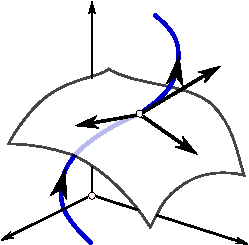
\includegraphics[width=\unitlength]{A28tangent3}}%
    \put(0.91612064,0.70682767){\color[rgb]{0,0,0}\makebox(0,0)[lb]{\smash{$\vel$}}}%
    \put(0.48698745,0.90266503){\color[rgb]{0,0,0}\makebox(0,0)[lb]{\smash{$\ssp(\zeit)$}}}%
    \put(0.2624318,0.5347756){\color[rgb]{0,0,0}\makebox(0,0)[lb]{\smash{$\groupTan_1$}}}%
    \put(0.80471037,0.38188675){\color[rgb]{0,0,0}\makebox(0,0)[lb]{\smash{$\groupTan_2$}}}%
    \put(0.538343,0.25344355){\color[rgb]{0,0,0}\makebox(0,0)[lb]{\smash{$\LieEl\ssp$}}}%
    \put(0.47864531,0.56060893){\color[rgb]{0,0,0}\makebox(0,0)[lb]{\smash{$\ssp$}}}%
  \end{picture}%
~~(b)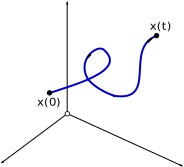
\includegraphics[width=0.20\textwidth]{A27traj}
\\
(c)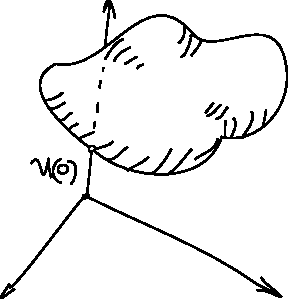
\includegraphics[width=0.20\textwidth]{A27gOrbit}
(d)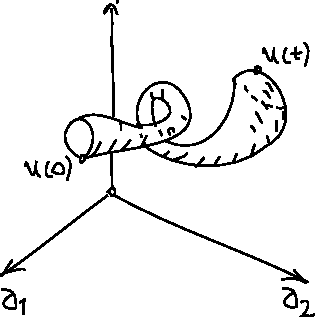
\includegraphics[width=0.20\textwidth]{A27wurst}
   \caption{\label{fig:A27wurst}
   (a)
In presence of $N$-continuous parameter symmetry, each \statesp\ point
$\ssp$ owns $(N\!+\!1)$ tangent vectors: one $\vel(\ssp)$ along the time
flow $\ssp(\zeit)$, and the $N$ group tangents  $\groupTan_1(\ssp), \,
\groupTan_2(\ssp) ,\,\cdots, \groupTan_N(\ssp)$ along infinitesimal
symmetry shifts, tangent to the group orbit $\LieEl\ssp$.
    (b)
Trajectory.
    (c)
Group orbit.
    (d)
Wurst.
}
\end{figure}
%%%%%%%%%%%%%%%%%%%%%%%%%%%%%%%%%%%%%%%%%%%%%%%%%%%%%%%%%%%%%%%%%%%%%

A flow $\map^t$ and the \statesp\ $\pS$ on which the flow acts comprise a
{dynamical system}. If a group $\Group$ of continuous transformations
acts on a continuous time flow, each \statesp\ point owns a set of
tangent vectors (\reffig{fig:A27wurst}\,(a)). Integrated globally, the
velocity vector $\vel(\ssp)$ traces out the {\em trajectory}
$\flow{\zeit}{\ssp}$ ( \reffig{fig:A27wurst}\,(b)). Applying the continuous
transformations traces out the {group orbit} (or, from now on, just
\emph{orbit})
\(
\pS_\ssp = \{\LieEl\,\ssp \mid \LieEl \in {\Group}\}
% \,,\qquad \pS_\ssp \subset \pS
\,
\) %ee{sspOrbit}
(\reffig{fig:A27wurst}\,(c)). Together they trace out a complicated smooth
manifold (hereafter affectionately referred to as the {\em wurst}, see
figures~\ref{fig:A27wurst}\,(d), \ref{fig:CLf01group}\,(b) and
\ref{fig:sliceimage}), that we shall teach you here how to slice.

A flow is said to have symmetry $\Group$ if the form of evolution
equations $\dot{\ssp} = \vel(\ssp)$ is left invariant,
\(
\vel(\ssp)=\LieEl^{-1} \, \vel(\LieEl \, \ssp)
% \,,\qquad \mbox{for all }
\,,
\) %ee{eq:FiniteRot}
by the set of transformations $\LieEl \in {\Group}$. Physicists love
symmetry, but Nature does not care: turbulence breaks all symmetries,
and while the flow equations may be invariant under $\Group$, their
solutions typically are not.

The key to chaotic dynamics is the notion of recurrence. To quantify how
close the state of the system now is to a previously visited state, we
need the notion of distance between two points in \statesp. The simplest
(but far from the only, or the most natural) is the Euclidean norm
\beq
  \Norm{\ssp-\ssp'}^2  = \braket{\ssp-\ssp'}{\ssp-\ssp'} =
\sum_j^d
(\ssp-\ssp')_j^2
\,.
\ee{innerproduct}
Given a notion of distance we can talk about 'neighborhood,' the open set of
nearby states. Our main task in what follows will be to make this precise,
by defining a chart over a neighborhood, and its borders.
Given distances and neighborhoods,
the next key notion is  \emph{measure}, or how likely a typical
trajectory is to visit a given neighborhood. After some observations of a
given turbulent flow, one can identify a set of representative
\emph{\template s}\rf{rowley_reconstruction_2000}, {points}
$\slicep{}^{(j)}$, $j=1,2,\cdots$ in the \statesp\ $\pS$, which are the
dynamically most important unstable {\recurrStr s} of the flow.
%    \DB{2012-04-12}{Neighborhoods not defined up to this point
%    in the text. Should they be? Predrag: done now.}

Our goals here are two-fold:
(i) In \refsect{s:cut} we review the method of \PoincSec s, with
    emphasis on aspects applicable to high-dimensional flows: construction of
    multiple local linear `charts' and determination of their borders and
(ii) in \refsect{s:slice} we show how the same set of tools applied to
    reduction of continuous symmetries enables us to commence a
    systematic charting of the long-time dynamics of high-dimensional
    flows with continuous symmetries (\refsect{s:chart}).

    \ifdraft\color{blue}
still to discuss:
\begin{itemize}

  % \item section {\PoincS} vs slice \pSRed

  \item strobing $\sim$ method of connections

  \item reduction vs projection
\end{itemize}
    \color{black}\fi


\section{\KSe}
\label{s-KS}
%\section{\KSe}
%\label{sec:KSe}

The \KS\ [henceforth KS] system was derived by
Kuramoto and Tsuzuki\rf{ku} as a phase equation for
reaction-diffusion systems described by Complex Ginzburg-Landau
equation and independently by Sivashinsky\rf{siv} to describe
instabilities in laminar flame fronts. It also appears
in a variety of contexts including thin falling
films and interfacial instabilities between
concurrent viscous fluids\rf{BenKS66,LinKS74}.
% For an instructive derivation from Complex Ginzburg-Landau
% equation \cf~\rf{}.
Our motivation for its study is that it is one of the simplest
nonlinear PDEs that exhibit features reminiscent of fluid
turbulence and thus it is a convenient system to test new ideas.

 In the formulation
adopted here, the time evolution of the `flame front velocity'
$u=u(x,t)$ %on a periodic domain $u(x,t) = u(x+L,t)$
is given by
\beq
  u_t = F(u) = -{\textstyle\frac{1}{2}}(u^2)_x-u_{xx}-u_{xxxx}
    \,,\qquad   x \in [-L/2,L/2]
    \,,
\ee{ks}
with appropriate boundary conditions, as discussed in \refsect{sec:KSbc}.
Here $t \geq 0$ is the time, and $x$ is the spatial coordinate.
The subscripts $x$ and $t$ denote partial derivatives with respect to
$x$ and $t$.

\subsection{Boundary conditions and system size}
\label{sec:KSbc}

Ideally we would like to work in a system of infinite spatial extend, \ie\ in the limit $L\rightarrow\infty$.
Although solutions of KS equations in this limit have appeared, \cf for example \refrefs{hooper_travelling_1988,feng_multiplicity_2004}\ES{More citations needed. Kevrekidis \etal\
mention criticism of periodic BC, but they give no reference.}, it is
more convenient, both computationally and theoretically, to work with periodic boundary conditions
\beq
  u(x,t) = u(x+L,t)\,,
 \label{eq:KSper}
\eeq
and this is the usual choice in the literature and the one followed in this thesis.
% The justification in terms of the physics
% of the problem is that we focus our attention to a small part of a larger system,
% far away from the boundaries. Further
Justification of this choice will be given
in \refsect{sec:KSeSymm}, in conjunction with the discussion of the symmetries of the system.

Another common choice of boundary conditions is
\beq
  u(0,t) = u(L,t)=0\,,
 \label{eq:KSodd}
\eeq
which restricts the system to the subspace of odd functions. This choice will also be discussed
in \refsect{sec:KSeSymm}.

In what follows
we shall state results of all calculations either in units of the system size $L$
or the `dimensionless system size' $\tildeL=L/2\pi$.
All numerical results presented in this thesis
are for $\tildeL=22/2\pi = 3.5014\ldots$, unless otherwise
noted. The system size leads to a system that is just ``turbulent'' enough
to have interesting dynamics, \cf \refsect{sec:L22}, while being still
rather tractable and can be used  as a test bed for
continuous symmetry reduction and a dynamical systems approach, see also \refsect{sec:ksSizeBC}.

\subsection{Symmetries of \KS\ system}
\label{sec:KSeSymm}

In an unbounded domain, $x\in(-\infty,\infty)$, KS equation is equivariant
under the action of the non-compact Euclidean group $\En{1}$:
If $u(x,t)$ is a solution, then
$\Shift({\shift})\, u(x,t) = u(x+\shift,t)$
is an equivalent solution for any shift
$\shift\in\Rls{}$, as is the reflection (`parity' or `inversion') $\Refl$ defined by
\beq
    \Refl \, u(x) = -u(-x)
\,.
\ee{KSparity}

Imposing periodic boundary conditions we restrict attention to the subspace
$[-L,L]$ in which only the compact subgroup \On{2} of \En{1} acts by:
\beq
	\Shift_{\shift/L}\, u(x,t) = u(x+\shift,t)\,,\qquad \shift\in\left[-L/2,L/2\right]	
	\label{KSshift}
\eeq
and reflections \refeq{KSparity}. Here we use subscript
notation for shifts to differentiate with the case of \En{1}.
Moreover, we only consider perturbations within this subspace,
\ie\ we do not consider subharmonic perturbations. The system
size $L$ affects the representation of \On{2}, \cf
\refsect{sec:fourKS}. \ES{This statement needs to be checked:
An important fact is that the isotropy subgroups of \En{1} (of
\En{n} in general) are all compact subgroups, if the action is
proper, see for example \refref{ChossLaut00}. Thus the
equivariant bifurcation structure as $L$ increases is not
affected, at least as long as we are not in the
spatio-temporally chaotic regime, when the spectrum of
stability eigenvalues becomes quasi-continuous.} Reflection
generates the dihedral subgroup $\Dn{1} = \{1, \Refl\}$ of
$\On{2}$. Boundary conditions \refeq{eq:KSodd} restrict the
system to \Fix{\Dn{1}} and thus in that case symmetry \Dn{1}
is impossed to all solutions. To avoid technical difficulties
associated with the action of \On{2} on an infinite dimensional
space we will discuss the isotropy subgroups of \On{2} in
\refsect{sec:ksIso}, after we truncate \refeq{expan} to finite
order.


The KS equation is also Galilean invariant: if $u(x,t)$ is a solution,
then $u(x -ct,t) -c $, with $c$ an arbitrary constant
speed, is also a solution. As one can verify by integrating \refeq{ks} with
respect to $x$ over the periodic domain $[-L/2,L/2]$ the quantity
 $\int_{-L/2}^{L/2} u\,dx$
is conserved and we can, without loss of generality, set it equal to zero. This corresponds
to the choice $c=0$, therefore eliminating Galilean invariance.


% $G$, the group of actions $ g \in G $ on a
% \statesp\ (reflections, translations, \etc) is a symmetry of the KS
% flow \refeq{ks} if $g\,u_t = F(g\,u)$.

% The KS equation is time translationally invariant, and space translationally invariant
% on a periodic domain under
% the 1-parameter group of
% $O(2): \{\Shift_{\shift/L},\Refl \}$.
% If $u(x,t)$ is a solution, then
% $\Shift_{\shift/L}\, u(x,t) = u(x+\shift,t)$
% is an equivalent solution for any shift
% $-L/2 < \shift \leq L/2$,
% as is the
% reflection (`parity' or `inversion')
% \beq
%     \Refl \, u(x) = -u(-x)
% \,.
% \ee{KSparity}

\subsection{Why $L=22$ on periodic domain?}
\label{sec:ksSizeBC}

For \KS\ system with periodic boundary conditions one expects to find
traveling wave (\reqv) and modulated amplitude traveling wave
(\rpo) solutions, exactly the kind of
solutions that we set out to understand and organize. Indeed,
a very detailed bifurcation study of such solutions for \KSe\
has been carried out by Brown and Kevrekidis\rf{BrKevr96},
see discussion in \refsect{sec:KSePO}. In our work the emphasis is
on working with a specific system size, with specific boundary
conditions, and determining and labeling all unstable periodic
and relative periodic solutions (up to a given topological
length). A bifurcation analysis is not practical for
such a task as global bifurcations that lead to creation and
disappearance of (relative) \po s are hard to track.
Therefore one needs to understand the geometry of phase space
in order to detect and organize the compact solutions
systematically.

The \KS\ system of size $L=22$ appears amenable to such a
geometric study, yet it provides new challenges. As we will
see in \refchap{chap:kseStSp}, many of the invariant objects
(\eqva, \reqva, {\po s}, {\rpo s}) have more than one
unstable eigendirections, a situation that has not been dealt
with in previous \KSe\ studies in terms of periodic
orbits\rf{Christiansen97,LanThesis,lanCvit07}, and which very
often occurs in the studies of \pCf\
\rf{GHCW07,HGC08,GHCV08,HalcrowThesis}. Nevertheless, the
system is not large enough to exhibit many unstable,
essentially non-separated (quasi-continuous) eigenvalues.
Systems with quasi-continuous spectra are known as
\emph{spatio-temporally chaotic} in the sense that they are
disordered both in space and in
time\rf{manneville_instabilities_2004} and a dynamical
description of such systems presents many more challenges
than we would like to be faced with while we try for the
first time to understand the organization of a flow in terms
of (modulated) traveling wave solutions.  The $L=22$ system
remains within reach of a dynamical description, see
\refchaps{chap:kseStSp}{chap:kseRedStSp}, while offering
valuable insight on how to deal with other, larger, more
turbulent or realistic systems.




\subsection{Fourier space}
\label{sec:fourKS}

\On{2} equivariance makes it convenient to work in Fourier space,
\beq
  u(x,t)=\sum_{k=-\infty}^{+\infty} a_k (t) e^{ i k x /\tildeL }
\,,
\ee{eq:ksexp}
with the $1$-dimensional PDE \refeq{ks}
replaced by an infinite set of
ODEs for the complex Fourier coefficients $a_k(t)$:
\beq
\dot{a}_k= \pVeloc_k(a)
     = ( q_k^2 - q_k^4 )\, a_k
    - i \frac{q_k}{2} \sum_{m=-\infty}^{+\infty} a_m a_{k-m}
\,,
\ee{expan}
where $q_k = k/\tildeL$.
Since $u(x,t)$ is real,
 \beq
  a_{k}=a^\ast_{-k} \,,
  \label{eq:astar}
 \eeq
and we can replace the
sum by a $k > 0$ sum. Note that $\dot{a}_0=0$ in
 \refeq{expan} as a result of Galilean invariance and $a_0$ is a conserved quantity
 fixed to $a_0=0$ by the condition $\int_{-L/2}^{L/2} u\,dx$=0.
In the Fourier basis \On{2} acts absolutely irreducibly on each complex plane
$\left(\Re(a_k),\Im(a_k)\right)$ and the linear part of \refeq{expan} is conveniently
diagonalized. Indeed, the translation operator action on the Fourier coefficients \refeq{eq:ksexp},
represented here by a complex valued vector
$a = \{a_k\in\mathbb{C}\,|\,k = 1, 2, \ldots\}$, is given by
\beq
  \Shift_{\shift/L}\, a = \mathbf{g}(\shift) \, a \,,
  \label{eq:shiftF}
\eeq
where $\mathbf{g}(\shift) = \mathrm{diag}( e^{i q_k\, \shift} )$ is a complex
valued diagonal matrix, which amounts to the $k$-th mode complex plane
rotation by an angle $k\, \shift /\tildeL$. The reflection acts on
the Fourier coefficients by complex conjugation and a change of sign,
\beq
  \Refl \, a = -a^\ast
\,.
\label{eq:FModInvSymm}
\eeq

\ES{This is from my first year KS special problem, perhaps some parts are usable:
Some qualitative comments about the KS equation can now be easily
given in view of \refeq{expan}. The linear behavior of the system
depends on the sign of the quantity $k^2- \left(2\pi/L\right)  k^4$.
For a sufficiently large system, the first few values of $k$ yield $k^2- \left(2\pi/L\right)
k^4>0$ or $k<\sqrt{L/2\pi}$ and the corresponding Fourier components grow exponentially
with time (unstable components). In other words the anti-diffusion
term in \refeq{eq:KS} (resulting in the term $\sim k^2$ in
\refeq{eq:Fcoef}) dominates over the dissipation term (resulting in
$\sim k^4$ in \refeq{eq:Fcoef}).  On the other hand there are infinitely many larger
wavenumber components with $k>\sqrt{L/2\pi}$ for which the solutions
are bounded (stable components). The role of the bilinear term in
\refeq{eq:Fcoef} is then to excite the larger wavenumber components
while dissipating the smaller wavenumber ones. The result of this
competition is that the asymptotic dynamics of the system are
confined on a low dimensional attractor.}


\subsection{Truncation}

Dynamical \statesp\ representation of a PDE is $\infty$-dimensional,
but the KS flow is strongly contracting and its non-wondering set,
and, within it, the set of invariant solutions investigated here, is
embedded into a finite-dimensional inertial manifold\rf{FNSTks85} in
a non-trivial, nonlinear way. The existence of an inertial manifold for
\KSe with both odd and periodic boundary conditions has been proved and
several bounds for its dimension have been found, \cf\ \refref{jolly_evaluating_2000} and references
therein. The best current bound in dimension of inertial manifold for KS
equation with periodic boundary condition is, to the author's knowledge,
given in \refrefs{Robinson_inertial_1994,jolly_evaluating_2000}: $O(L^{2.46})$ for $L\in[2\pi,6\pi]$.

The fact that the asymptotic dynamics lies on a finite
dimensional manifold justifies truncation of the infinite tower
of equations \refeq{expan} to finite order $N$. According to
the bound $O(L^{2.46})\simeq2000$ for $L=22$\ES{$L=22>6\pi$, so
it looks like their proof does not apply to our system if one
wants to be rigorous.} and we would expect to need even more
Fourier modes, since the Fourier basis is not directly
connected to coordinates on the inertial manifold of KSe and
would therefore be less optimal than an approach that
approximates such coordinates, for
example\rf{Jolly_approximate_1990,JRT01}.
Nevertheless such a bound seems rather inflated compared to
numerical simulations of the asymptotic dynamics that typically
require $O(10)-O(100)$ Fourier modes. In practice we keep
$16\leq N \leq 128$ Fourier modes in numerical simulations and
check the robustness of the results against increase of $N$.

\subsection{Isotropy lattice and invariant subspaces}
\label{sec:ksIso}

Let $N$ be the number of Fourier modes retained in \refeq{expan}
and observe that the action of $O(2)$
on \Rls{N} by \refeq{eq:shiftF} and \refeq{eq:FModInvSymm} is,
up to the minus sign in \refeq{eq:FModInvSymm}, identical
to the action \refeq{eq:O2stndrd} of \On{2} on \Clx{N} studied
in \refsect{sec:strata}.
The isotropy lattice remains unchanged but \fixedsp s of the dihedral subgroups are affected.
\Fixedsp s of \Cn{q}, given by the condition
\beq
	a_k=0\ \mathrm{unless}\ k = q j\,,\ j=1,\ldots\lfloor n/q \rfloor\,,
	\label{eq:O2ksCqFix}
\eeq
remain unchanged but the \fixedsp s of the dihedral subgroups \Fix{\Dn{m}} are now given by the conditions
\bea
	a_k=0\ \mathrm{unless}\ k = m j\,,\ j=1,\ldots\lfloor n/m \rfloor\,, \\
	\Re(a_k)=0\ \mathrm{for}\ k=1,\ldots,n\,.
	\label{eq:O2ksDqFix}
\eea
In relation to physical space we observe that \Fix{\Dn{1}} is the subspace of antisymmetric functions $Re(z_k)=0,\, \forall k$ or $u(-x)=-u(x)$ while for the action \refeq{eq:O2stndrd} the corresponding
subspace would be that of symmetric functions.

\subsection{\Eqva\ and their bifurcations}
\label{sec:ksBif}

%%%%%%%%%%%%%%%%%%%%%%%%%%%%%%%%%%%%%%%%%%%%%%%%%%%%%%%%%%%%%%%%%%
\begin{figure}[ht]
\begin{center}
  (\textit{a})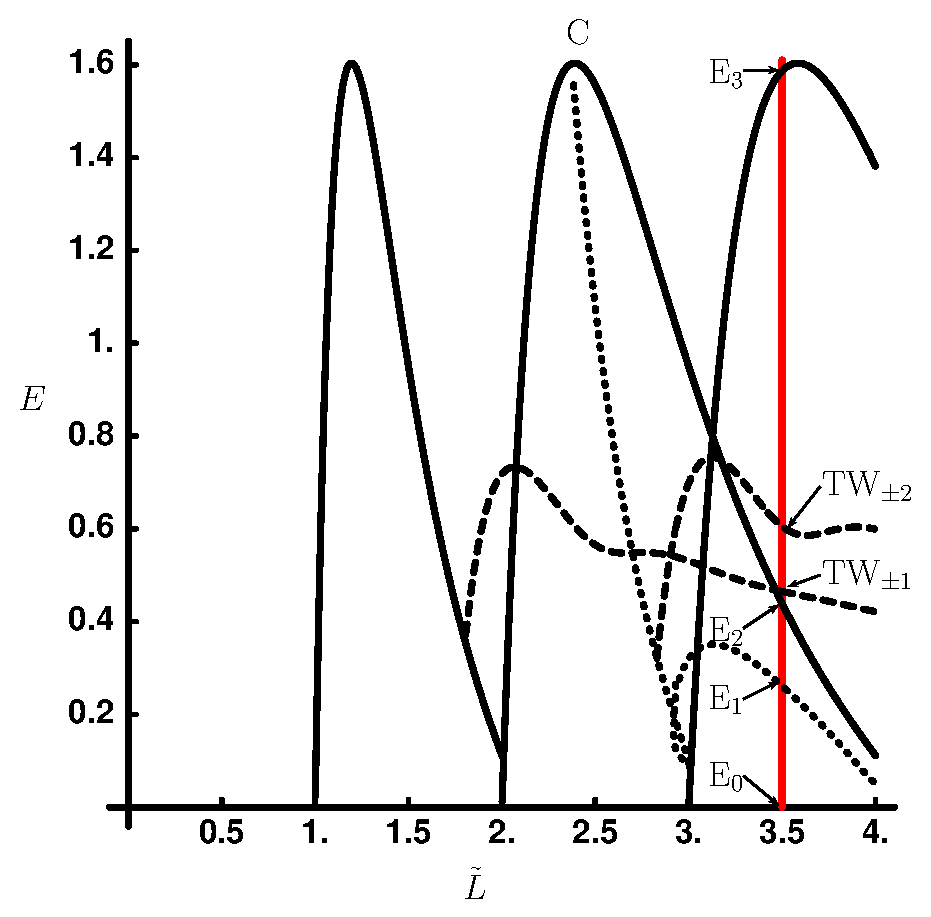
\includegraphics[width=0.5\textwidth]{../figs/ksBifDiag}
\end{center}
\caption[KS steady state bifurcations]{
The energy \refeq{ksEnergy} of the \eqva\ and \reqva\ that
exist up to $L=22$, $\tildeL = 3.5014\ldots$, plotted as a function
of the system size $\tildeL = L/2\pi$ (additional \eqva, not present
at $L = 22$ are given in \refref{ksgreene88}). Solid curves denote
$n$-cell solutions \EQV{2} and \EQV{3}, dotted curves the GLMRT
\eqv\ \EQV{1},
and dashed curves the \reqva\ \REQV{\pm}{1} and \REQV{\pm}{2}.
The parameter $\alpha$ of \refrefs{KNSks90,ksgreene88} is
related to the system size by $\tildeL=\sqrt{\alpha/4}$.    }
\label{fig:ksBifDiag}
\end{figure}
%%%%%%%%%%%%%%%%%%%%%%%%%%%%%%%%%%%%%%%%%%%%%%%%%%%%%%%%%%%%%%%%

\Eqva\  (or the steady solutions)
are the fixed profile time-invariant solutions,
\beq
 u(x,t) = u_\stagn(x)
\,.
\ee{eqva}
Due to the translational symmetry,
the KS system also allows for
\reqva\ (traveling waves, rotating waves),
characterized by a fixed profile $u_\stagn(x)$
moving with constant speed $c$, {\ie}
\beq
 u(x,t) =  u_\stagn(x-ct)
\,.
\ee{reqva}
Here suffix ${}_\stagn$ labels a particular invariant solution.
Because of the reflection symmetry \refeq{KSparity},
the \reqva\ come in counter-traveling pairs
$u_\stagn(x-ct)$, $-u_\stagn(-x+ct)$.

The \reqv\ condition for the {\KS} PDE \refeq{ks}
is the ODE
\beq
{\textstyle\frac{1}{2}}(u^2)_x+u_{xx}+ u_{xxxx}=c \, u_x
\ee{KSeqvCond}
which can be analyzed as a dynamical system in its own right.
Integrating once we get
\beq
{\textstyle\frac{1}{2}}u^2 - c u + u_x + u_{xxx}=\expctE
\,.
\label{eq:stdks}
\eeq
This equation can be interpreted as a 3-dimen\-si\-on\-al dynamical system
with spatial coordinate $x$ playing the role of `time,'
and the integration constant \expctE\ can be interpreted as `energy,'
see \refsect{sec:energy} and \reffig{fig:ksBifDiag}.

In the Fourier representation the \reqva\ time dependence is
\beq
 a_k(t) e^{-itc q_k} = a_k(0)
\,.
\ee{reqvaF}
Differentiating with respect to time, we obtain
the Fourier space version of the \reqv\ condition
\refeq{KSeqvCond},
\beq
 \pVeloc_k(a) - i q_k c a_k = 0
\,,
\ee{reqvCondF}
which we solve for (time independent) $a_k$ and $c$, see \refchap{chap:kseStSp}.

In a periodic box of size $L$
both \eqva\ and \reqva\ are  periodic solutions
embedded in 3-$d$ space, conveniently represented as loops in
$(u,u_x,u_{xx})$ space, see \reffig{f:KS22Equil}\,(\textit{d}).
In this representation the continuous translation symmetry
is automatic -- a rotation in the $[0,L]$ periodic domain only
moves the points along the loop. For an \eqv\ the points
are stationary in time; for \reqv\ they move in time, but in
either case, the loop remains invariant.
% So we do not have the problem that we encounter in the Fourier
% representation, where seen from the frame of one of the \eqva\
% the rest trace out circles under the action of continuous symmetry
% translations.
Unfortunately this visualization has not helped
our understanding of \KSe\ state space.

The  \eqva\ and \reqva\ of KS equation and their bifurcations have been
the object of extensive study and a literature survey
cannot be exhaustive. The results of relevance for this thesis can be
found in \refrefs{Mks86,laquey74,ksgreene88,KNSks90,AGHks89}.
Although these results were obtained by direct bifurcation
analysis rather than with methods of equivariant
bifurcation theory, the relation of bifurcations to \On{2}
symmetry has been recognized in the literature particularly in
\refrefs{KNSks90,AGHks89}. The relation of the bifurcations
found numerically (and in some cases analytically) in
\refref{KNSks90} to the predictions of equivariant bifurcation
theory is discussed in Krupa\rf{Krupa90} but
without explicit calculations. In this section we describe some
of the elementary and well known bifurcations in KS equation
from the point of view of equivariant bifurcation theory.

 Since the origin (u(x,t)=0 in physical space) is the \fixedsp\ of \On{2} it is,
by \refPro{pro:gfInv}, flow invariant and thus
an \eqv. From commutation relation \refeq{eq:LrzCommut} we conclude that the
linear stability matrix (see \refsect{sec:ksReal}) $A(0)$
and the representation of the symmetry group \On{2} share a complete
set of eigenvectors, the Fourier modes.
% From relation \refeq{eq:LrzCommut} $A(0)$ has to commute
% with the generator of rotations, which in real Fourier basis becomes
% \beq
% \begin{array}{lll}
%  & × & × \\
% × & × & × \\
% × & × & ×
% 	  \end{array}
% \)
% \eeq
Moreover, since \On{2} acts absolutely irreducibly
on each Fourier plane $A(0)$ is diagonal (in real Fourier basis)
with eigenvalues $\lambda_0^{(k)}=( q_k^2 - q_k^4 )$, from \refeq{expan}.
For $L<2\pi$
the origin is linearly stable and due to the hyperviscous damping $u_{xxxx}$ it is the global
attractor\rf{KNSks90}. At $L=2\pi$ the origin loses stability and due
to the diagonal form of $A(0)$ the kernel of the linearization is immediately seen to be the
$k=1$ irreducible subspace. Taking into account the orthogonality of the Fourier basis, the Lyapunov-Schmidt reduction \cite{golubitsky2002sp} is automatic and we can work in the $k=1$ subspace (\cf ``Restriction Lemma'' in \refref{KNSks90}
for technical details). In this subspace all requirements
of Equivariant Branching Lemma \cite{golubitsky2002sp}\ES{write, add refThe.} are satisfied: $\On{2}$ acts
absolutely irreducibly, $v_1(a)$ is equivariant (Lyapunov-Schmidt reduction respects symmetry),
the eigenvalue crossing condition holds $\frac{d}{d L}\lambda_0^{(1)}(2\pi)\neq 0$, and
finally $\Dn{1}$ is an axial subgroup since \Fix{\Dn{1}} is the imaginary axis in the complex $a_1$ plane.
Therefore there is a unique solution branch of \eqva\ in \Fix{\Dn{1}}, \ie\ with symmetry $\Dn{1}$.
% \ES{After secondary bifurcations it appears that the branch does not remain in \Dn{1}, check.}
This is known as the unimodal branch in the literature. The stability of the bifurcating \eqv\
can not be determined from symmetry arguments and one has to take into account the evolution equations
\refeq{expan}. The unimodal \eqv\ is stable at bifurcation\rf{KNSks90}. Under the action of $\Shift$ we
get a continuous family of \eqva\ for any \eqv\ in $D_1$.

The bifurcation scenario repeats itself each time $L=2\pi k$: The $k$'th mode eigenvector of
the origin looses stability and an \eqv\ with symmetry $D_k$ is born, giving rise to
the $k$-modal branch. The Lyapunov-Schmidt reduction and application of Equivariant branching lemma
carries through in exactly the same way. In \refref{KNSks90} the observation is made that one
can get the k-modal branch from the unimodal through the substitution $u(x)\mapsto u(kx)$
and therefore the $k$-modal branches are called k-fold replications
of the unimodal branch, \cf\ also \refref{Krupa90}. Note that the k-modal branch
with $k>1$ ``inherits'' the unstable directions of the origin and thus are born unstable at the
bifurcation. In \refref{ksgreene88} states in the $k$-modal branch are called $k$-cell states.
Condition \refneq{eq:O2ksDqFix} implies that in these states only the Fourier modes $a_j$ where $j$
is a multiple of $k$ are non zero. Each $k$-modal branch merges with the $2k$-modal branch, see \reffig{fig:ksBifDiag}
and \refrefs{KNSks90,ksgreene88}. Note that, according to \refexam{O2iso}, $\Fix{\Dn{1}}\supset\Fix{\Dn{k}}$
for all $k$, so all unimodal \eqva\ are antisymmetric.

The replication observed in primary bifurcations is not carried to the secondary bifurcations that are
much richer. From here on we only consider bifurcations that play a role in the dynamics for our system size, $L=22$, see \reffig{fig:ksBifDiag}. The $\EQV{2}$ and $\EQV{3}$ indicated in that diagram belong
in the bimodal and trimodal branches, respectively.

The $1$-cell state loses stability and bifurcates to a branch of stable
\reqva, which later on becomes unstable through a Hopf bifurcation\rf{KNSks90,ksgreene88}.
This is the branch indicated as $\REQV{\pm}{1}$ in \reffig{fig:ksBifDiag}. Since \reqva\ are not in \Fix{\Dn{1}}
and they are invariant, as a set, under translations \refneq{eq:shiftF}, they have to come in copies
under the action of \Dn{1}. The sign in $\REQV{\pm}{1}$ indicates direction of rotation, see \refeq{reqva}.
\PublicPrivate{}{For a discussion of relation of this bifurcation to Krupa's theorem, see \refref{Krupa90}.}%end \PublicPrivate

At point $C$ in \reffig{fig:ksBifDiag} the $2$-cell state
bifurcates to a type of \eqv\ solution found by La Quey,
Mahajan, Rutherford and Tang\rf{laquey74} and generalized by
Greene and Kim who refer to them as GLMRT \eqva. In
\refref{KNSks90} this branch of solutions is refered to as
bi-tri branch as it is later on terminated at the trimodal
branch. Bi-tri \eqva\ live in \Fix{\Dn{1}} and have components
in all Fourier modes\ES{Is this symmetry increasing
bifurcation?}. At the point where the bi-tri branch meets the
trimodal branch a new branch is born that is still in
\Fix{\Dn{1}}. This is seen as a continuation of the bi-tri
branch in \refref{KNSks90}. The \eqv\ labeled \EQV{1} in
\reffig{fig:ksBifDiag} is in this branch.

Finally the \reqv\ that is labeled \REQV{\pm}{2} belongs to a branch bifurcating from the bi-tri branch in
a Hopf bifurcation. Once again the \reqva\ come in \Dn{1} related, counter-traveling pairs.


% \ES{I think there is a symmetry we have missed. It looks like the unstable eigenvectors of
% \EQB{3} are in \Cn{3} on which rotations act and therefore after reduction we get one unstable
% eigendirection. This explains the multiplicity of the eigenvalue and maybe the shape of its
% unstable manifold.}


\PublicPrivate{}{

For $\expctE>0$ there is rich
$\expctE$-dependent dynamics, with
fractal sets of bounded solutions investigated in
depth by Michelson\rf{Mks86}.
For $\tildeL<1$ the only \eqv\ of the system is the
globally attracting constant
solution $u(x,t)=0$, denoted $\EQV{0}$ from now on. With increasing system size $L$ the system
undergoes a series of bifurcations.
The resulting \eqva\ and
\reqva\ (but not \po s and \rpo s)
are described in the classical papers of
Kevrekidis, Nicolaenko and Scovel\rf{KNSks90},
and Greene and Kim\rf{ksgreene88}.
The relevant bifurcations
up to the system size
investigated here are summarized
in \reffig{fig:ksBifDiag}:
at $\tildeL=22/2\pi =
3.5014\cdots$, the {\eqva} are the constant solution
\EQV{0}, the GLMRT\rf{laquey74,ksgreene88} \eqv\ \EQV{1}, the $2$-
and $3$-cell states \EQV{2} and \EQV{3},
and the pairs of \reqva\ \REQV{\pm}{1}, \REQV{\pm}{2}.

Periods of spatially periodic {\eqva} are multiples of $L$.
Every time the system size crosses  $\tildeL=n$,
$n$-cell states
are generated through pitchfork bifurcations off $u =0$
\eqv.
Due to the translational invariance of {\KSe},
they form invariant circles
in the full \statesp.
In the $\bbUplus$ subspace considered here,
they correspond to $2n$ points, each shifted by $L/2n$.
For a sufficiently small $L$
the number of {\eqva} is small and
concentrated on the low wave-number end of the Fourier spectrum.

From \refeq{expan} we see that the origin $u(x,t) = 0$
has Fourier modes as the linear stability eigenvectors
(see Appendix~\ref{sec:stability}).  The $|k|<\tildeL$
long wavelength perturbations of the flat-front {\eqv}
are linearly unstable, while all
$|k|> \tildeL$ short wavelength perturbations are strongly contractive.
The high $k$ eigenvalues, corresponding to rapid variations of
the flame front, decay so fast that the corresponding eigendirections
are physically irrelevant.
The most unstable mode, nearest to $|k|=\tildeL/\sqrt{2}$,
sets the scale of the mean wavelength $\sqrt{2}$
of the KS `turbulent' dynamics,
see \reffig{f:ks_largeL}.
}%end \PublicPrivate



\subsection{\Rpo s and \po s} \label{sec:KSePO}

% The KS equation \refeq{ks} is time translationally invariant, and
% space translationally invariant under the 1-$d$ Lie group of $O(2)$
% rotations: if $u(x,t)$ is a solution, then $u(x+\shift,t)$ and
% $-u(-x,t)$ are equivalent solutions for any $-L/2 < \shift \leq
% L/2$.
As a result of invariance under $\Shift_{\shift/L}$,
KS equation can have \rpo\ solutions
with a profile $u_p(x)$, period $\period{p}$, and a
nonzero shift $\shift_p$
\beq
  \Shift_{\shift_p/L}u(x,\period{p}) =
  u(x+\shift_p,\period{p}) = u(x,0) = u_p(x)\,.
\label{KSrpos}
\eeq
{\Rpo s} \refeq{KSrpos} are periodic in
$v_p=\shift_p/\period{p}$ co-rotating frame (see
\reffig{f:MeanVelocityFrame}), but in the stationary frame their
trajectories are quasiperiodic.  Due to the reflection symmetry
\refeq{KSparity} of KS equation, every {\rpo} $u_p(x)$ with shift
$\shift_p$ has a symmetric partner $-u_p(-x)$ with shift $-\shift_p$.
In Fourier space we have:
\beq
  {\bf g}(\shift_p)f^\period{p}(a_p) - a_p = 0\,,
\ee{eq:system}
with ${\bf g}$ as in \refeq{eq:shiftF}.

\PublicPrivate{}{
As $\shift$ is continuous in the interval $[-L/2, L/2]$,
the likelihood of a \rpo\ with $\shift_p = 0$ shift is zero,
unless an exact periodicity is enforced by a discrete symmetry,
such as the dihedral symmetries discussed above.
If the shift $\shift_p$ of a \rpo\ with period $\period{p}$ is such
that $\shift_p /L$ is a rational number, then the orbit is
periodic with period $n\period{p}$.  The likelihood to find such \po s is
also zero.
}

KS equation can also have periodic solutions
characterized by a profile $u_p(x)$,
and period $\period{p}$. In terms of symmetry it is easier to think of them
in (truncated) Fourier space. For any discrete\footnote{Recall from \refExa{O2iso} that \On{2} fixes the origin, so
we cannot have periodic orbits with spatial symmetry \On{2}.} subgroup in the isotropy lattice
we can have periodic solutions with spatial symmetry \Dn{k} or \Cn{k}. For all $\gamma$ in \Dn{k} or \Cn{k}.
\beq
  \gamma a_p(t) = a_p(t)\,, \qquad  \forall t\in[0,\period{p}]\,.
\eeq
Such a solution lives in \Fix{\Dn{k}} of \Fix{\Cn{k}}.
% or in the terminology of Golubitsky and Stewart\rf{golubitsky2002sp},
% it has spatial symmetry \Dn{k}.
The periodic orbits found in \refrefs{Christiansen97,lanCvit07}, for example,
are all in \Fix{\Dn{1}}, as a result of restricting the dynamics to that subspace by the choice of antisymmetric
boundary conditions. In our case, for $L=22$, the dynamics in \Fix{\Dn{1}} are dominated by attracting (within
the subspace) heteroclinic connections and thus we have no periodic orbits of this type, or in
any other of the \Fix{\Dn{k}} subspaces, see \refchap{chap:kseStSp}. Moreover spatial symmetries have to
be in the isotropy lattice, see Chapter~3 of \refref{golubitsky2002sp} so there are no more possibilities
for orbits with just spatial symmetry.

The second type of periodic orbits would have spatio-temporal symmetry
with spatial part a discrete subgroup in the isotropy lattice
$\stab{a_p(t)}=\Dn{k}$ or \Cn{k} and trivial spatial symmetry.
% In the terminology of Chapter~3 of \refref{golubitsky2002sp} we would
% say that the spatial part of the spatio-temporal symmetry is
% \Dn{k} or \Cn{k} and there are no spatial symmetries.
Yet, due
to algebraic restrictions on possible spatio-temporal
symmetries, see Chapter~3 of \refref{golubitsky2002sp}, the
spatial part has to be cyclic and thus we are left with
$\Dn{1}$ and $\Cn{k}$ as our possibilities. For our system
size, $L=22$, we have found no periodic orbits with isotropy
subgroup $\Cn{k}$, see \refchap{chap:kseStSp}. We have found
periodic orbits with isotropy subgroup $\Dn{1}$, period
$\doubleperiod{p}$, which satisfy
\beq
	\Refl a(t+\period{p})=a(t)\,,
	\label{eq:ppo}
\eeq
where $\period{p}=\doubleperiod{p}/2$ by the relation $\kappa^2=e$. We choose to label those
periodic orbits with the half-period $\period{p}$ because this will be the period in the $O(2)$-reduced space,
where the segment of the orbit for time $[\period{p},\doubleperiod{p}]$ is a repeat of the \emph{prime} segment
for $[0,\period{p}]$. Thus we will refer to those orbits as pre-periodic of period $\period{p}$.
Periodic orbits \refeq{eq:ppo} live in the principal stratum and thus their group orbit under translations \refeq{eq:shiftF} is a manifold of equivalent solutions. Returning to physical space we have
\beq
  \Refl u(x+\shift,\period{p}) =
  -u(-x-\shift,\period{p}) = u(x+\shift,0) = u_p(x)
  \,,
\label{KSpos}
\eeq
the family of equivalent solutions
parameterized by $\shift$
(as the choice of the reflection point is arbitrary,
the shift can take any value in $-L/2 < \shift \leq L/2$).
\PublicPrivate{}{
However, due to the KS equation invariance under reflection \refeq{KSparity},
two types of \po s are possible:

{\bf (a)} The \po\ lies within the  $\bbUplus$ antisymmetric subspace,
$-u_p(-x) = u_p(x)$, and $u(x,\period{p}) = u(x,0) = u_p(x)$.

{\bf (b)} If an
orbit is of reflection type \refeq{KSpos},
$\Refl\Shift_{\shift/L} u(x,\period{p}) =
-u(-x-\shift,\period{p}) = u(x,0)$, then it is
pre-periodic to a \po\ with period
$2\period{p}$.
Indeed, since $(\Refl\Shift_{\shift/L})^2 = \Refl^2 = 1$,
 and the KS solutions
are time translation invariant, it follows
from \refeq{KSpos} that
\[
  u(x,2\period{p}) = \Refl\Shift_{\shift/L} u(x,\period{p}) =
  (\Refl\Shift_{\shift/L})^2 u(x,0) = u(x,0)\;.
\]
Thus any shift acquired during time $0$ to
$\period{p}$ is compensated by the opposite shift during
evolution from $\period{p}$ to $2 \period{p}$.
}% end PublicPrivate
Such pre-periodic orbits
are a hallmark of any dynamical system with a discrete
symmetry, where they have a natural
interpretation as \po s in the
fundamental domain\rf{CvitaEckardt,DasBuch}.

Brown and Kevrekidis\rf{BrKevr96} study bifurcations branches
of \rpo s for a wide range of system sizes $L$ for \KSe. For
our system size they identify two \rpo\ branches.
They are
created when either a heteroclinic cycle (see \refchap{chap:kseStSp})
or \reqv\ becomes unstable, see also \refrefs{Krupa90,AGHO288,AGHks89}.
In \refref{BrKevr96} partially hyperbolic invariant tori are also found
for larger systems, see \refchap{chap:tobedone}.

\section{Energy transfer rates}
\label{sec:energy}

In physical settings where the observation times are much longer than
the dynamical `turnover' and Lyapunov times (statistical mechanics,
quantum physics, turbulence) periodic orbit theory\rf{DasBuch} provides
highly accurate predictions of measurable long-time averages such as
the dissipation and the turbulent drag\rf{GHCW07}. Physical predictions have to be
independent of a particular choice of ODE representation of the PDE
under consideration and, most importantly, invariant under all
symmetries of the dynamics. In this section we discuss a set of such
physical observables for the  1-$d$ KS invariant under reflections and
translations. They offer a representation of dynamics in which the
symmetries are explicitly quotiented out. We shall use these observable in
\refsect{sec:energyL22} in order to visualize a set of solutions on
these coordinates. They implement
symmetry reduction, but their utility, as we will see in \refsect{sec:energyL22},
has been limited.

The {space average} of a function $\obser = \obser(\pSpace,t) = \obser(u(x,t))$  on
the interval $L$,
\beq
    \expct{\obser} = \Lint{\pSpace}\, \obser(\pSpace,t)
    \,,
    \label{rpo:spac_ave}
\eeq
is in general time dependent.
Its mean value is given by the {time average}
\beq
\timeAver{\obser}
    =
\lim_{t\rightarrow \infty} \frac{1}{t} \int_0^t \! d\tau \, \expct{\obser}
    =
\lim_{t\rightarrow \infty} \frac{1}{t} \int_0^t \!
    \Lint{\tau}  d\pSpace\, \obser(\pSpace,\tau)
    \,.
\label{rpo:tim_ave}
\eeq
The mean value of $\obser = \obser(u_\stagn) \equiv \obser_\stagn$ evaluated on $q$
\eqv\ or {\reqv} $u(\pSpace,t) = u_\stagn(\pSpace-ct)$ is
\beq
\timeAver{\obser}_\stagn = \expct{\obser}_\stagn = \obser_\stagn\,.
\label{rpo:u-eqv} \eeq Evaluation of the infinite time average
\refeq{rpo:tim_ave} on a function of a \po\ or \rpo\
$u_p(\pSpace,t)=u_p(\pSpace,t+\period{p})$ requires only a single
$\period{p}$ traversal,
\beq
  \timeAver{\obser}_p = \frac{1}{\period{p}}
    \int_0^{\period{p}} \! d\tau \, \expct{\obser}
\,.
\label{rpo:u-cyc}
\eeq

Equation \refeq{ks} can be written as
\beq
    u_t=- V_x
        \,,\qquad
    V(x,t)={\textstyle\frac{1}{2}}u^2+u_{x} + u_{xxx}
    \,.
\ee{ksPotent} If $u$ is `flame-front velocity' then \expctE, defined in
\refeq{eq:stdks}, can be interpreted as the mean energy density.
So, even though KS is a phenomenological
small-amplitude equation, the time-dependent quantity
\beq
    \expctE=
  \Lint{\pSpace}
  V(x,t)=
  \Lint{\pSpace} \frac{u^2}{2}
  \label{ksEnergy} \eeq
has a physical interpretation\rf{ksgreene88} as the average `energy'
density of the flame front. This analogy to the mean kinetic energy
density for the Navier-Stokes motivates what follows.

The energy \refeq{ksEnergy} is intrinsic to
the flow, independent of the particular ODE basis set
chosen to represent the PDE. However, as the Fourier
amplitudes are eigenvectors of the translation operator,
in the Fourier space the energy is a diagonalized
quadratic norm,
\beq
\expctE
          =  \sum_{k=-\infty}^{\infty} E_k
\,,\qquad
E_k =
    {\textstyle\frac{1}{2}}|a_k|^2
\,,
\ee{EFourier}
and explicitly invariant term by term
under translations
\refeq{eq:shiftF}
and reflections \refeq{KSparity}.

Take time derivative of the energy density \refeq{ksEnergy},
substitute \refeq{ks} and integrate by parts. Total derivatives vanish
by the spatial periodicity on the $L$ domain:
\bea
   \dot{\expctE} &=&
     \expct{u_t \, u}
         = - \expct{\left({u^2}/{2} + u \, u_{x} + u \, u_{xxx}\right)_x u }
    \continue
    &=&
\expct{ u_x \, {u^2}/{2} + u_{x}{}^2 + u_x \, u_{xxx}}
    \,.
\label{rpo:ksErate}
\eea
The first term in \refeq{rpo:ksErate} vanishes by
integration by parts,
\(
3 \expct{ u_x \, u^2}= \expct{(u^3)_x} = 0
\,,
\)
and integrating the third term by parts yet again
one gets\rf{ksgreene88} that the energy variation is
\beq
   \dot{\expctE} = P - D
                \,,\qquad
      P =  \expct{u_{x}{}^2}
                \,,\quad
      D =  \expct{u_{xx}{}^2}\,.
\ee{EnRate}
The power $P$ pumped in by anti-diffusion $u_{xx}$ is
balanced by the energy dissipation rate $D$ due
hyper-viscosity $u_{xxxx}$ in the KS equation \refeq{ks}.

The time averaged energy density  $\timeAver{E}$
computed on a typical orbit goes to a constant, so
the expectation values \refeq{rpo:EtimAve} of drive and dissipation
exactly balance each out:
\beq
    \timeAver{\dot{E}}  =
    \lim_{t\rightarrow \infty}
        \frac{1}{t} \int_0^t d\tau \, \dot{\expctE}
=
      \timeAver{P} - \timeAver{D}
= 0
    \,.
\ee{rpo:EtimAve}
In particular, the \eqva\
and \reqva\ fall onto the diagonal in \reffig{f:drivedrag},
and so do time averages computed on \po s and \rpo s:
\beq
\timeAver{E}_p =
\frac{1}{\period{p}} \int_0^\period{p}d\tau \, E(\tau)
    \,,\qquad
\timeAver{P}_p =
\frac{1}{\period{p}} \int_0^\period{p} d\tau \, P(\tau)
    =
      \timeAver{D}_p
    \,.
\label{poE}
\eeq
In the Fourier basis \refeq{EFourier} the conservation of energy on average
takes form
\beq
0 = \sum_{k=-\infty}^{\infty} ( q_k^2 - q_k^4 )\,
    \timeAver{E}_k
\,,\qquad
E_k(t) =  {\textstyle\frac{1}{2}} |a_k(t)|^2
\,.
\ee{EFourier1}
The large $k$ convergence of this series is insensitive to the
system size $L$; $\timeAver{E_k}$ have to decrease much faster than
$q_k^{-4}$.
Deviation of $E_k$ from this bound for small $k$ determines the active modes.
For \eqva\ the $L$-independent bound
    on $E$ is given by Michaelson\rf{Mks86}.
The best current bound\rf{GiacoOtto05,bronski2005} on the long-time limit
of $E$
as a function of the system size $L$ scales as
$E \propto L^{3/2}$.

One can go on constructing similar quantities in
order to obtain a symmetry invariant basis for the system by
considering higher moments. Yet, the procedure is tedious and
the physical significance of higher moments unclear so we
will not pursue this further. We will nevertheless use the
$E,\,P$ and $D$ basis for visualization in
\refchap{chap:kseStSp} to emphasize both its utility as a
readily available symmetry invariant representation and its
limitations and need for a better basis.


\section{Energy transfer rates} % of the \KSe}
\label{sec:energy}
% energy.tex
% $Author$ $Date$


% \section{Representation in terms of symmetry invariant moments} % of the \KSe}
% \label{sec:energy}
% Predrag                   Apr 12 2007

In physical settings where the observation times are much longer
than the dynamical `turnover' and Lyapunov times (statistical mechanics,
quantum physics, turbulence)
periodic orbit theory\rf{DasBuch}
provides highly accurate predictions of measurable
long-time averages such as the turbulent drag\rf{GHCW07}.
Physical predictions have to be independent of a
particular choice of ODE representation of
the PDE under consideration
and, most importantly,
invariant under all symmetries of the dynamics.
In this section we discuss
a set of such physical observables for
the  1$D$ KS invariant under reflections and translations.
They offer a representation of
dynamics in which the symmetries are explicitly quotiented out.
We illustrate  this in  \refsect{sec:energyL22} by projecting
a set of explicit solutions on these coordinates.

The {space average} of a function $\obser = \obser(\pSpace,t)$  on
the interval $L$,
\beq
    \expct{\obser} = \Lint{\pSpace}\, \obser(\pSpace,t)
    % \expct{\obser} = \frac{1}{L}\int_0^{L} d\pSpace\, \obser(\pSpace,t)
    \,,
    \label{rpo:spac_ave}
\eeq
is in general time dependent.
Its mean value is given by the {time average}
\beq
\timeAver{\obser}
    =
\lim_{t\rightarrow \infty} {1\over t} \int_0^t \! d\tau \, \expct{\obser}
    =
\lim_{t\rightarrow \infty} {1\over t} \int_0^t \!
    \Lint{\tau}  d\pSpace\, \obser(\pSpace,\tau)
    \,.
\label{rpo:tim_ave}
\eeq
The mean value
% $\timeAver{\obser}$,
of $\obser = \obser(u_\stagn) \RLDedit{\equiv \obser_\stagn}$ evaluated on
$q$ \eqv\ or {\reqv} $u(\pSpace,t) = u_\stagn(\pSpace-ct)$ is
\beq
%         \obser_\stagn = \timeAver{\obser}_\stagn = \expct{\obser}_\stagn
\RLDedit{\timeAver{\obser}_\stagn = \expct{\obser}_\stagn = \obser_\stagn }
\,.
\label{rpo:u-eqv}
\eeq
Evaluation of the infinite time average \refeq{rpo:tim_ave}
on a function of a
\po\ or \rpo\ $u_p(\pSpace,t)=u_p(\pSpace,t+\period{p})$
 requires only a single $\period{p}$
traversal,
\beq
       \RLDedit{\timeAver{\obser}_p} = \frac{1}{\period{p}}
    \int_0^{\period{p}} \! d\tau \, \expct{\obser}
\,.
\label{rpo:u-cyc}
\eeq

Equation \refeq{ks} can be written as % in ``potential'' form
\beq
    u_t=- V_x
        \,,\qquad
    V(x,t)={\textstyle\frac{1}{2}}u^2+u_{x} + u_{xxx}
    \,.
\ee{ksPotent}
$u$ is related to the `flame-front height' $h(x,t)$ by
$u=h_x$, so \expctE \RLDedit{, defined in \refeq{eq:stdks},}
can be interpreted as the mean energy density.
% \refeq{ksEnergy}.
%
So, even though KS is a phenomenological
small-amplitude equation, the time-dependent quantity
\beq
    \expctE=
%\frac{1}{L}\int_0^{L} \!dx \,
\RLDedit{\Lint{\pSpace}}
V(x,t)=
%\frac{1}{L}\int_0^{L}\! dx \,
\RLDedit{\Lint{\pSpace}}
\frac{u^2}{2}
\label{ksEnergy}
\eeq
has a physical interpretation\rf{ksgreene88}
as the average `energy' density of the flame front.
This analogy to the corresponding definition of the
mean kinetic energy density for
the Navier-Stokes motivates what follows.

The energy \refeq{ksEnergy} is intrinsic to
the flow, independent of the particular ODE basis set
chosen to represent the PDE. However, as the Fourier
amplitudes are eigenvectors of the translation operator,
in the Fourier space the energy is a diagonalized
quadratic norm,
\beq
\expctE   % = (u,u)
          = \sum_{k=1}^{\infty} E_k
\,,\qquad
E_k = % a_{-k} a_k =
    {\textstyle\frac{1}{2}}|a_k|^2
\,,
\ee{EFourier}
and explicitly invariant term by term
under translations \refeq{eq:RPOcondFouri}.

Take time derivative of the energy density \refeq{ksEnergy},
substitute \refeq{ks} and integrate by parts. Total derivatives vanish
by the spatial periodicity on the $L$ domain:
\bea
   \dot{\expctE} &=&
     \expct{u_t \, u}
    % \frac{1}{L}\int_0^{L}u \, u_t\, dx
     = - \expct{\left({u^2}/{2} + u \, u_{x} + u \, u_{xxx}\right)_x u }
    \continue
    &=&
\expct{ u_x \, {u^2}/{2} + u_{x}{}^2 + u_x \, u_{xxx}}
    \,.
\label{rpo:ksErate}
\eea
The first term in \refeq{rpo:ksErate} vanishes by
integration by parts,
\(
3 \expct{ u_x \, u^2}= \expct{(u^3)_x} = 0
\,,
\) % {EnNonl0}
and integrating the third term by parts yet again
one gets\rf{ksgreene88} that the energy variation
\beq
   \dot{\expctE} = P - D
                \,,\qquad
      P =  \expct{u_{x}{}^2}
                \,,\quad
      D =  \expct{u_{xx}{}^2}
\ee{EnRate}
balances the power $P$ pumped in by anti-diffusion $u_{xx}$
against the energy dissipation rate $D$
by hyper-viscosity $u_{xxxx}$
in the KS equation \refeq{ks}.

The time averaged energy density  $\timeAver{E}$
computed on a typical orbit goes to a constant, so
the expectation values \refeq{rpo:EtimAve} of drive and dissipation
exactly balance each out:
\beq
    \timeAver{\dot{E}}  =
    \lim_{t\rightarrow \infty}
        {1\over t} \int_0^t d\tau \, \dot{\expctE}
=
      \timeAver{P} - \timeAver{D}
%       \timeAver{(u_{x})^2} - \timeAver{(u_{xx})^2}
= 0
    \,.
\ee{rpo:EtimAve}
In particular, the \eqva\
and \reqva\ fall onto the diagonal in \reffig{f:drivedrag},
and so do time averages computed on \po s and \rpo s:
\beq
\timeAver{E}_p =
{1\over \period{p}} \int_0^\period{p}d\tau \, E(\tau)
    \,,\qquad
\timeAver{P}_p =
{1\over \period{p}} \int_0^\period{p} d\tau \, P(\tau)
    =
      \timeAver{D}_p
% \timeAver{(u_{x})^2}_p =
% {1\over \period{p}} \int_0^\period{p} d\tau \, \expct{(u_{x})^2}
%     =
%       \timeAver{(u_{xx})^2}_p
    \,.
\label{poE}
\eeq
In the Fourier basis \refeq{EFourier} the conservation of energy on average
takes form
\beq
0 = \sum_{k=1}^{+\infty} ( (k/\tildeL)^2 - ( k/\tildeL)^4 )\,
    \timeAver{E_k}
\,,\qquad
E_k(t) =  |a_k(t)|^2
\,.
\ee{EFourier1}
The large $k$ convergence of this series is insensitive to the
system size $L$; $\timeAver{E_k}$ have to decrease much faster than
$(k/\tildeL)^{-4}$.
\PC{determine the decay rate, presumably exponential in $k$}
Deviation of $E_k$ from this bound for small $k$ determines the active modes.
This may be useful to bound the number of equilibria, with
the upper bound given by zeros of a small number
of long wavelength modes.
For \eqva\ the $L$-independent bound
    on $E$ is given by Michaelson\rf{Mks86}.
The best current bound\rf{GiacoOtto05,bronski-2005} on the long-time limit
of $E$
as a function of the system size $L$ scales as
$E \propto L^{3/2}$.
%
\PC{
 % Past: Michael Loss has not taught us how to bound $E$ by
 %  Sobolev bounds. Neither has Spiegel. Next: But
  Constantin says that the answer is in
    \refrefs{temam85ks}. Eckmann says: the  best bound is by Otto\rf{GiacoOtto05}; the
    only bound close to k=0, better in essential way. See also \refref{bronski-2005}.
    Eckmann had $L^{8/5}$, but conceptually Otto is the best. Recheck whether it is
    $|u|$ or $E \propto L^{3/2}$.
    When the solution is big, how long can it stay big? They found it cannot stay big for
    long.
       }
\PC{
from bounds on energy, we might be able
to bound the number of equilibria as function of systems size $L$, and thus
be sure we have them all.
   }
%
\PC{Next for fluid guys: read Lieb and Ruelle to learn
    how to bound $E$ for plane Couette by Sobolev bounds}


\section{Geometry of state space with $L=22$}
\label{sec:L22}
% L22eqv.tex
% $Author$ $Date$

\section{Geometry of state space with $L=22$}
\label{sec:L22}

We now turn to exploring Hopf's vision
numerically, on a specific \KS\ system.
An instructive example is offered by the dynamics for
the  $L=22$  system
that we specialize to for the rest of this paper.
The size of this
small system is $\sim 2.5$ mean wavelengths
($\tildeL/\sqrt{2}= 2.4758\ldots$),
and the competition between states with wavenumbers 2 and 3
leads to the empirically observed `sustained turbulence'.
Asymptotic attractor structure of small systems like
the one studied here
is very sensitive to system parameter variations, and,
as is true of
any realistic unsteady flow, there is no rigorous way of
establishing that this `turbulence' is sustained for all time,
rather than being
merely a very long transient on a way to an
attracting periodic state.
For large system size, as the one shown in \reffig{f:ks_largeL}, it is
hard to imagine a scenario under which attractive periodic states
(as shown in \refref{FSTks86}, they do exist) would have significantly
large immediate basins of attraction.
Regardless of the
(non)existence of a $t \to \infty$ chaotic attractor, study
of the invariant unstable solutions and the associated Smale
horseshoe structures in system's \statesp\ offers valuable
insights into the observed unstable `coherent structures.'

Because of the strong $k^4$ contraction, for a small system size
one expects that the long-time dynamics is confined to low-dimensional
center manifold. Indeed, numerically the leading Lyapunov exponents of the
$L=22$ chaotic attractor are
$(\Lyap_i) = (0.048, 0, 0, -0.003, -0.189, -0.256, -0.290, \cdots)$,
so the chaotic dynamics mostly takes
place close to a 4-dimensional manifold, with strong
contraction in other dimensions.  The two zero exponents
are due to the
time and space translational symmetries of the \KSe,
and it was shown in \refrefs{Christiansen97,LanCvi07}
that within particular curvilinear coordinate frames, the
dynamics on the attractor can sometimes be reduced to
local 1- or 2-dimensional maps.
Hence a relatively small
number of Fourier modes, typically 128 used in numerical calculations presented here,
suffices to obtain
numerically accurate (within $10^{-5}$) invariant
solutions.

We next investigate the properties of \eqva\ and \reqva\ and determine numerically
a large set of the short periods \rpo s for KS in a periodic cell of
size $L=22$.

\section{\Eqva\ and \reqva\ for $L=22$}

In addition to the trivial \eqv\ $u=0$ (denoted \EQV{0}),
we find three \eqva\ with dominant wavenumber $k$
(denoted \EQV{k}) for $k = 1, 2, 3$.  All {\eqva}, shown in
Fig.~\ref{f:KS22Equil}, are symmetric with respect to the reflection
symmetry \refeq{KSparity}.
In addition, \EQV{2} and \EQV{3} are symmetric with respect
to translation \refeq{KSshift}, by $L/2$ and $L/3$, respectively.
\EQV{2} and \EQV{3} essentially lie, respectively, in
the 2$^\mathrm{nd}$ and 3$^\mathrm{rd}$ Fourier component complex plane,
with small $k=2j$, $k=3j$ harmonics deformations.

%%%%%%%%%%%%%%%%%%%%%%%%%%%%%%%%%%%%%%%%%%%%%%%%%%%%%%%%%%%%%%%%%%
\begin{figure}[t]
\begin{center}
  (\textit{a})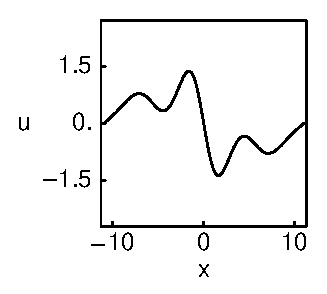
\includegraphics[width=0.35\textwidth]{figs/1wKS22equil.eps}
~~~~(\textit{b})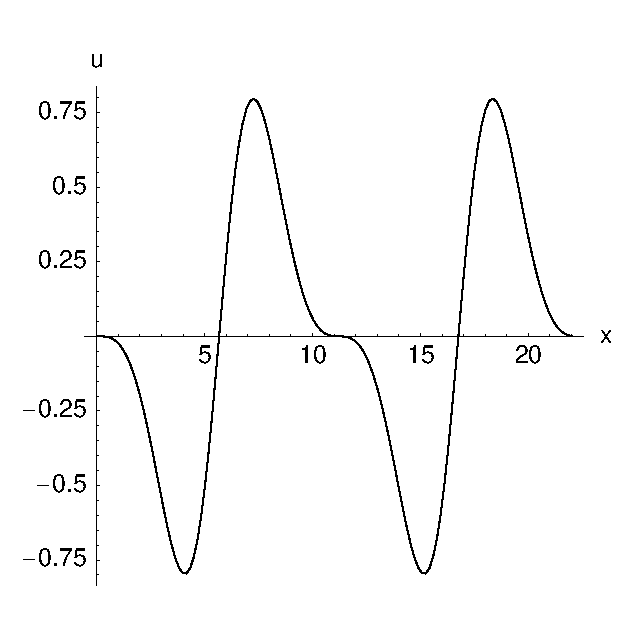
\includegraphics[width=0.35\textwidth]{figs/2wKS22equil.eps}
\\
  (\textit{c})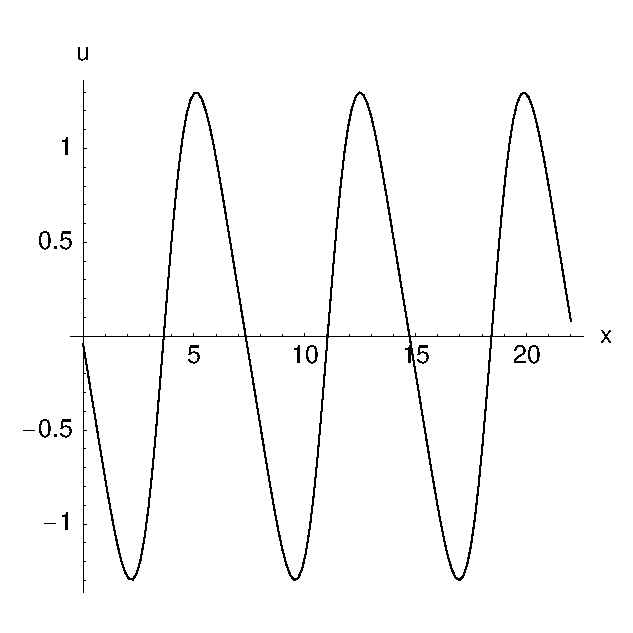
\includegraphics[width=0.35\textwidth]{figs/3wKS22equil.eps}
~~~~(\textit{d})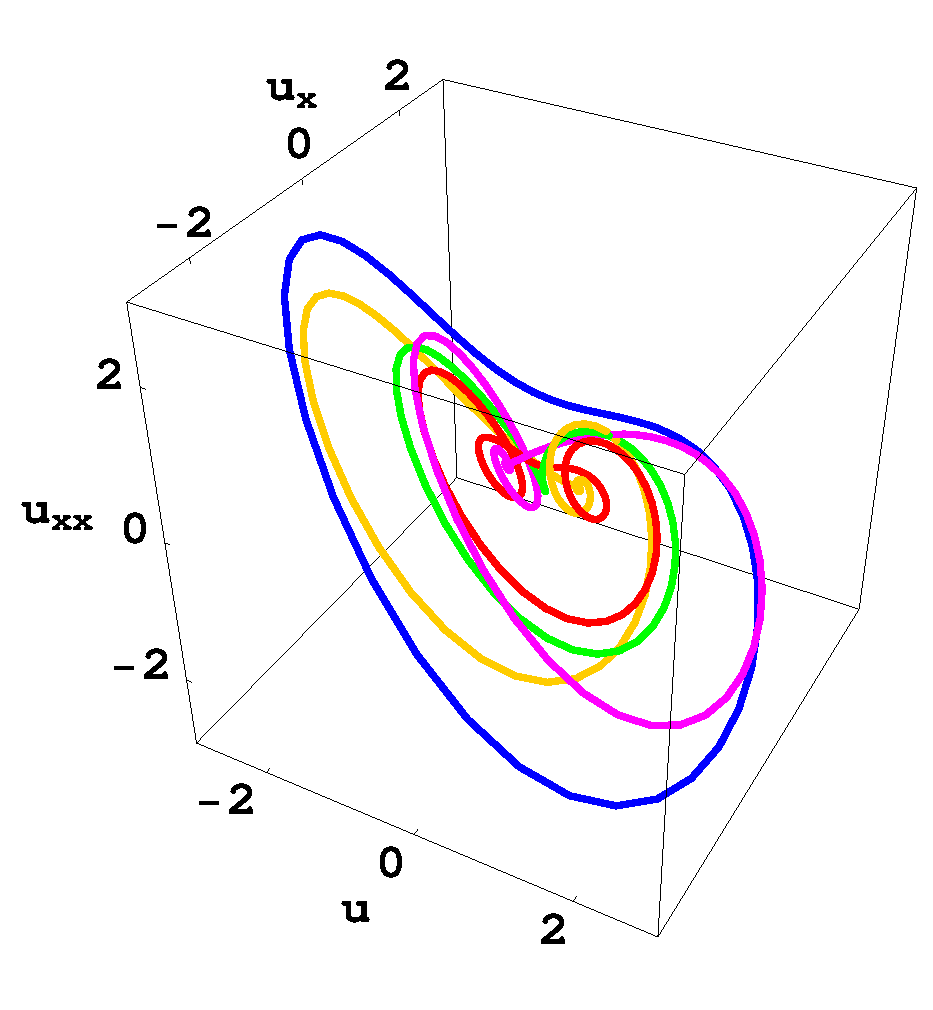
\includegraphics[width=0.35\textwidth]{figs/equilSpatial.eps}
\end{center}
\caption{
(a) \EQV{1}, (b) \EQV{2}, and (c)
\EQV{3} \eqva. The \EQV{0} \eqv\ is the $u(x)=0$ solution.
(d) $(u,u_x,u_{xx})$ representation
of (red) \EQV{1}, (green) \EQV{2},  (blue) \EQV{3} \eqva,
(purple) \REQV{+}{1},  and (orange) \REQV{-}{1} \reqva.
$L=22$ system size.
    }
\label{f:KS22Equil}
\end{figure}
%%%%%%%%%%%%%%%%%%%%%%%%%%%%%%%%%%%%%%%%%%%%%%%%%%%%%%%%%%%%%%%%

The stability of the {\eqva} is characterized by the eigenvalues
$\eigExp[j]$ of the \stabmat.  The leading 10 eigenvalues for each
\eqv\ are listed in \reftab{tab:Eksym}. We have computed (available upon request)
the corresponding eigenvectors as well. As an \eqv\ with $\mathrm{Re}\,
\lambda_j > 0$ is unstable in the direction of the corresponding
eigenvector $\jEigvec{j}$, the eigenvectors provide flow-intrinsic
(PDE discretization independent) coordinates which we use for visualization
of unstable manifolds and homo/heteroclinic connections between
\eqva.

The eigenvalues of \EQV{0} are determined by the linear part of the KS
equation \refeq{expanMvar}: $\lambda_k=(k/\tilde{L})^2-(k/\tilde{L})^4$.
For $L=22$, there are three pairs of unstable eigenvalues, corresponding,
in decreasing order, to three unstable modes $k=2,3$, and 1.  For each
mode, the corresponding eigenvectors lie in the plane spanned by
$\Re \, a_k$ and $\Im \, a_k$. \refTab{tab:Eksym}
lists the symmetries of the stability eigenvectors of
\eqva\ \EQV{1} to \EQV{3}.

\begin{figure}[t]
\begin{center}
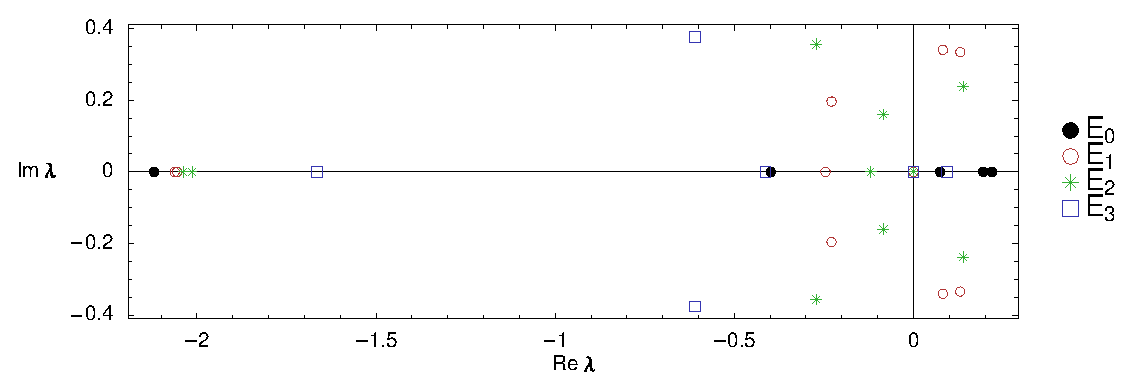
\includegraphics[width=4in]{figs/L22-eqvaEigenvalues.eps}
\end{center}
\caption{
Leading  \eqv\ stability eigenvalues,
$L=22$ system size.
}
\label{f:KS22EkEigs}
\end{figure}

\begin{table}[t]
\caption{
Leading eigenvalues
$\eigExp[j]= \eigRe[j] \pm i\eigIm[j]$
and symmetries of the corresponding eigenvectors
of KS {\eqva} and \reqva\ for $L = 22$ system size.
We have used as our reference states the ones that lie within
the antisymmetric subspace  $\bbU^+$,
and also listed the symmetries of
the $L/4$ translated ones.
        }\label{tab:Eksym}
\begin{center} \footnotesize
\begin{tabular}{ccccc}
\EQV{1}& $\eigRe[j]$ & $\eigIm[j]$ & Symmetry & $\Shift_{1/4}\EQV{n}$ Symmetry\\\hline
  $\eigExp[1,2]$ & $\ \ 0.1308$& $0.3341$ & -  & -\\
  $\eigExp[3,4]$ & $\ \ 0.0824$& $0.3402$ & $\bbU^+$  & $\bbU^{(1)}$\\
  $\eigExp[5]$   & $0$     &          & -  & -\\
  $\eigExp[6,7]$ &$-0.2287$& $0.1963$ & $\bbU^+$  & $\bbU^{(1)}$\\
  $\eigExp[8]$   &$-0.2455$&          & -  & -\\
  $\eigExp[9]$   &$-2.0554$&          & $\bbU^+$  & $\bbU^{(1)}$\\
  $\eigExp[10]$  &$-2.0619$&          & -  & -\\[2ex]
\EQV{2}&  &  & \\\hline
  $\eigExp[1,2]$ & $\ \ 0.1390$& $0.2384$ & $\bbU^+$         & $\bbU^{(1)}$\\
  $\eigExp[3]$   & $0$      &          & $\Shift_{1/2}$        & $\Shift_{1/2}$\\
  $\eigExp[4,5]$ &$-0.0840$ & $0.1602$ & $\bbU^{(1)}$           & $\bbU^+$\\
  $\eigExp[6]$   &$-0.1194$ &          & $\Shift_{1/2}$        & $\Shift_{1/2}$\\
  $\eigExp[7,8]$ &$-0.2711$ & $0.3563$ & $\bbU^+,\,\bbU^{(1)},\,\Shift_{1/2}$  & $\bbU^+,\,\bbU^{(1)},\,\Shift_{1/2}$\\
  $\eigExp[9]$   &$-2.0130$ &          & $\bbU^{(1)}$           & $\bbU^+$\\
  $\eigExp[10]$  &$-2.0378$ &          & $\bbU^+$         & $\bbU^{(1)}$\\[2ex]
\EQV{3}&  &  & \\\hline
  $\eigExp[1]$   &$\ \ 0.0933$&          & $\bbU^+$     & $\bbU^{(1)}$\\
  $\eigExp[2]$   &$\ \ 0.0933$&          & -         & -  \\
  $\eigExp[3]$   &$0$       &          & $\Shift_{1/3}$    & $\Shift_{1/3}$\\
  $\eigExp[4]$   &$-0.4128$ &          & $\bbU^+,\,\Shift_{1/3}$  & $\bbU^{(1)},\,\Shift_{1/3}$\\
  $\eigExp[5,6]$ &$-0.6108$ & $0.3759$ & $\bbU^+$     & $\bbU^{(1)}$\\
  $\eigExp[7,8]$ &$-0.6108$ & $0.3759$ & -         & -\\
  $\eigExp[9]$   &$-1.6641$ &          & -         & -\\
  $\eigExp[10]$  &$-1.6641$ &          & $\bbU^+$     & $\bbU^{(1)}$ \\[2ex]
$\REQV{\pm}{1}$&  &  & \\\hline
  $\eigExp[1,2]$ & $\ \ 0.1156$ & $0.8173$ & -  & -\\
  $\eigExp[3,4]$ & $\ \ 0.0337$ & $0.4189$ & -  & -\\
  $\eigExp[5]$   & $0$      &          & -  & -\\
  $\eigExp[6]$   &$-0.2457$ &          & -  & -\\
  $\eigExp[7,8]$ &$-0.3213$ & $0.9813$ & -  & -\\[2ex]
$\REQV{\pm}{2}$&  &  & \\\hline
  $\eigExp[1]  $ & $\ \ 0.3370$ &          & -  & -\\
  $\eigExp[2]  $ & $0$      &          & -  & -\\
  $\eigExp[3,4]$ &$-0.0096$ & $0.6288$ & -  & -\\
  $\eigExp[5,6]$ &$-0.2619$ & $0.5591$ & -  & -\\
  $\eigExp[7,8]$ &$-0.3067$ & $0.0725$ & -  & -\\
\end{tabular}
\end{center}
\end{table}


%%%%%%%%%%%%%%%%%%%%%%%%%%%%%%%%%%%%%%%%%%%%%%%%%%%%%%%%%%%%%%%%%%
\begin{figure}[t]
\begin{center}
\includegraphics[width=0.3\textwidth]{figs/ks22_TW1_profile.eps}
\includegraphics[width=0.3\textwidth]{figs/ks22_TW2_profile.eps}\\
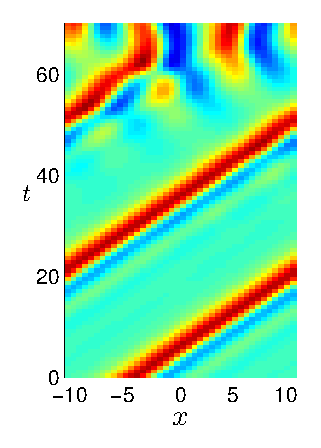
\includegraphics[width=0.3\textwidth]{figs/ks22_TW1_orbit_c.eps}
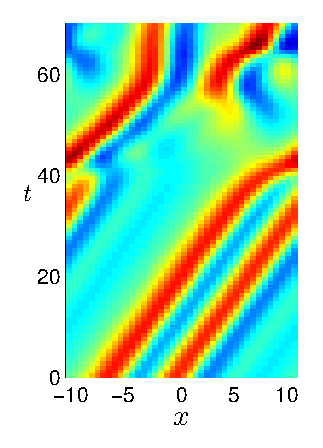
\includegraphics[width=0.3\textwidth]{figs/ks22_TW2_orbit_c.eps}
\end{center}
\caption{
\Reqva : \REQV{+}{1} with velocity $c = 0.737$ and \REQV{+}{2} with
velocity $c = 0.350$.
The upper panels show the \reqva\ profiles.  The lower panels show
evolution of slightly perturbed \reqva\ and their decay into generic
turbulence. Each \reqv\ has a reflection symmetric partner related by
$u(x) \to -u(-x)$ travelling with velocity $-c$.
} \label{f:ks22TW}
\end{figure}
%%%%%%%%%%%%%%%%%%%%%%%%%%%%%%%%%%%%%%%%%%%%%%%%%%%%%%%%%%%%%%%%%%

Consistent with the bifurcation diagram of \reffig{fig:ksBifDiag},
we find two pairs of \reqva\ \refeq{reqva} with velocities
$c =\pm 0.73699$ and $\pm 0.34954$
which we label \REQV{\pm}{1} and \REQV{\pm}{2},
for `traveling waves'.
The profiles of the two \reqva\ and their time evolution
with eventual decay into the chaotic attractor are
shown in \reffig{f:ks22TW}.  The leading eigenvalues of
\REQV{\pm}{1} and \REQV{\pm}{2} are listed in \reftab{tab:Eksym};
those with $\eigRe > -2.5$ are also plotted in
\reffig{f:KS22EkEigs}.

\refTab{tab:L22cminus} lists \eqv\ energy $E$,
the local Poincar\'e section return time $T$,
radially expanding Floquet multiplier $\ExpaEig_e$, and
the least contracting Floquet multiplier $\ExpaEig_c$
for all $L=22$ \eqva\ and \reqva.
The return time $T=2\pi/\eigIm[e]$ is given by the imaginary
part of the leading complex eigenvalue,
the expansion
multiplier per one turn of the most unstable spiral-out by
$\ExpaEig_e\approx\exp(\eigRe[e] T)$, and the contraction
rate along the slowest contracting stable eigendirection by
$\ExpaEig_c\approx\exp(\eigRe[c]T)$. We learn that the shortest
`turn-over' time is $\approx 10-20$, and that if there exist
horseshoe sets of unstable \po s associated with
these \eqva,  they have unstable
multipliers of order of $\ExpaEig_e \sim 5-10$, and that
they are surprisingly thin in the folding direction, with
contracting multipliers of order of $10^{-2}$,
as also observed in \refref{LanCvi07}.

\begin{table}[ht]
    \caption{
    Properties of \eqva\ and \reqva\ determining
    the system dynamics in their vicinity.  $T$ is characteristic
    time scale of the dynamics, $\ExpaEig_e$ and $\ExpaEig_c$ are the
    leading expansion and contraction rates, and $E$ is the
    energy \refeq{ksEnergy}.
            }
\begin{center} \footnotesize
    \begin{tabular}{l|rrrr}
                 & $E$~~   & $T$~~  & $\ExpaEig_e$  & $\ExpaEig_c$  \\ \hline
 $\EQV{1}\ $     &\ 0.2609 &\ 18.81 &\ 4.79     &\ 0.04 \\
 $\EQV{2}\ $     &\ 0.4382 &\ 26.35 &\ 5.99     &\ 0.03 \\
 $\EQV{3}\ $     &\ 1.5876 &\ 10.71 &\ 9.92     &\ 0.01 \\
 $\REQV{\pm}{1}$ &\ 0.4649 &  &  & \\
 $\REQV{\pm}{2}$ &\ 0.6048 &  &  & \\
    \end{tabular}
\end{center}
\label{tab:L22cminus}
\end{table}

\subsection{Unstable manifolds of \eqva\ and their heteroclinic
            connections}
\label{sec:unstMnflds}

As shown in \refTab{tab:Eksym},
the \EQV{1} \eqv\ has two unstable
planes within which the solutions are spiralling out (\ie, two
pairs of complex conjugate eigenvalues).  The \EQV{2} has one such plane,
while the \EQV{3} has two real positive eigenvalues, so the solutions are
moving radially away from the \eqv\ within the plane spanned
by the corresponding eigenvectors.  Since \EQV{1} has
a larger unstable subspace, it is expected to have much less influence on the
long time dynamics compared to \EQV{2} and \EQV{3}.

\begin{figure}[t]
\begin{center}
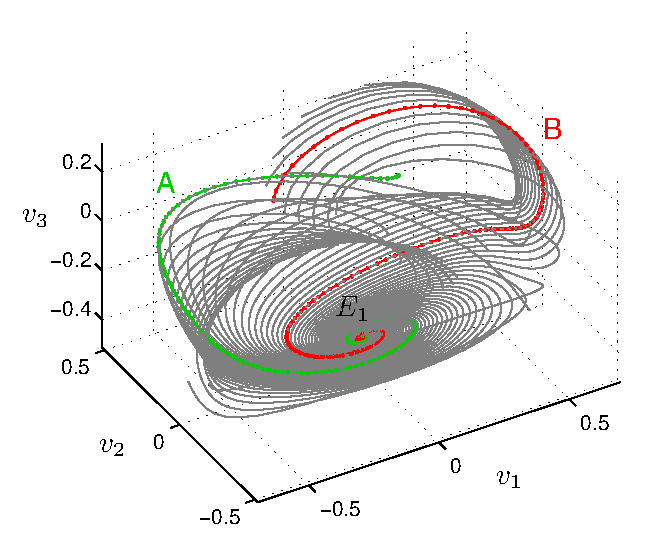
\includegraphics[width=0.5\textwidth]{figs/ks22_E1_plane1_manifold_c.eps}
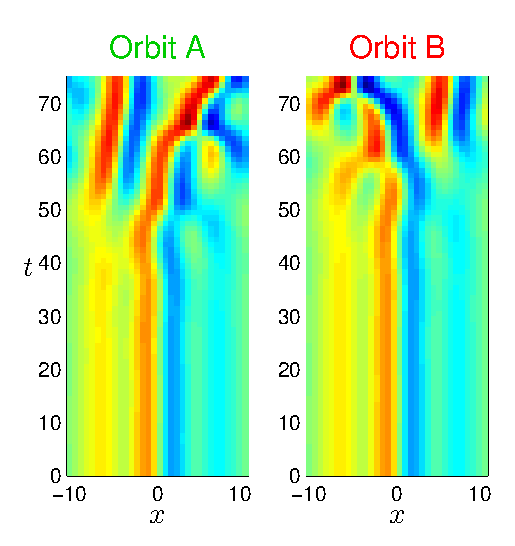
\includegraphics[width=0.4\textwidth]{figs/ks22_E1_plane1_orbits_c.eps}
\end{center}
\caption{
The left panel shows the unstable
manifold of \eqv\ \EQV{1} starting within the plane
corresponding to the first pair of unstable eigenvalues. The
coordinate axes $v_1$, $v_2$, and $v_3$ are constructed from vectors
$\Re \,\jEigvec{1}$, $\Im \,\jEigvec{1}$,
and $\Re \,\jEigvec{6}$
by Gram-Schmidt orthogonalization.
The right panel shows spatial representation of two orbits $A$ and $B$.
The change of color from blue to red indicates increasing values of
$u(x)$.
}
\label{f:KS22E1man1}
\end{figure}

To construct an invariant manifold containing solutions
corresponding to the pair of unstable complex conjugate eigenvalues,
$\eigExp = \eigRe \pm i\eigIm$,
$\eigRe > 0$, we start with a set of
initial conditions near \eqv\ \EQV{k},
\beq
  a(0) = a_{{\EQV{k}}} + \epsilon\,\exp(\delta)\jEigvec{j}
\,,
\ee{linUnstMan}
where $\delta$ takes the set of values uniformly distributed in the
interval $[0,2\pi\eigRe/\eigIm]$, $\jEigvec{j}$ is a unit vector in the
unstable plane, and $\epsilon > 0$ is small.

\begin{figure}[t]
\begin{center}
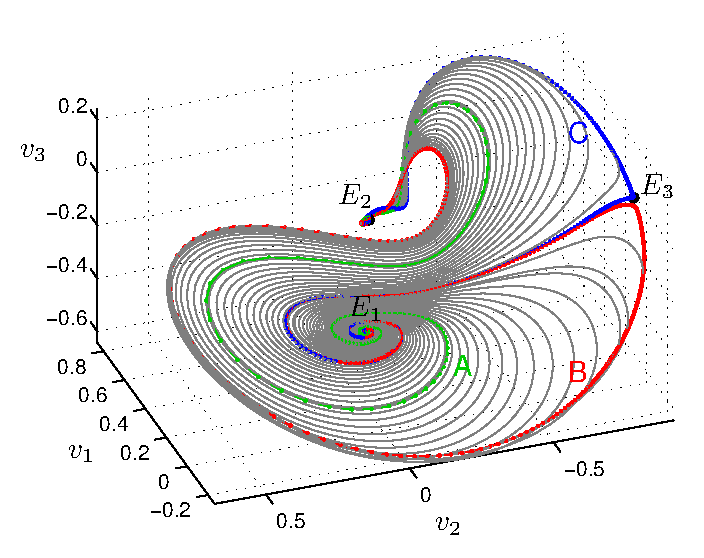
\includegraphics[width=0.48\textwidth]{figs/ks22_E1_plane2_manifold_c.eps}
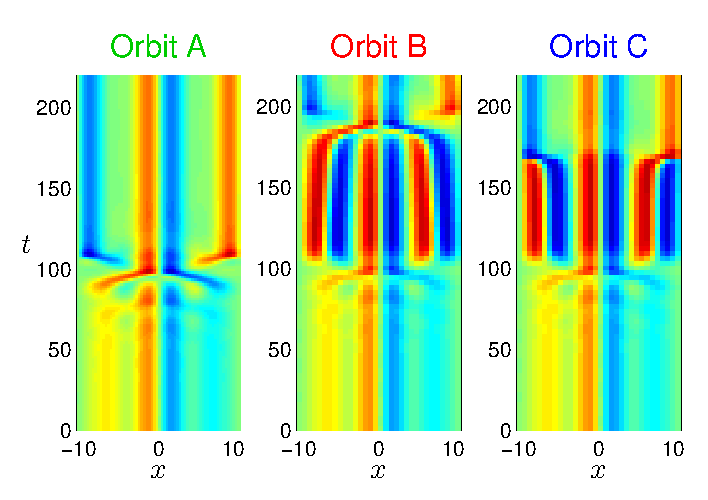
\includegraphics[width=0.48\textwidth]{figs/ks22_E1_plane2_orbits_c.eps}
\end{center}
\caption{
The left panel shows the unstable
manifold of \eqv\ \EQV{1} starting within the plane
corresponding to the second pair on unstable eigenvalues. The
coordinate axes $v_1$, $v_2$, and $v_3$ are constructed from vectors
\Re\, $\jEigvec{3}$, \Im\, $\jEigvec{3}$, and \Re\, $\jEigvec{6}$
by Gram-Schmidt orthogonalization.
The right panel shows spatial representation of three orbits. Orbits
$B$ and $C$ pass close to the \eqv\ \EQV{3}.
   }
\label{f:KS22E1man2}
\end{figure}

The manifold starting within the first unstable plane of \EQV{1}, with
eigenvalues $0.1308\pm i\,0.3341$, is shown in
\reffig{f:KS22E1man1}. It appears to fall directly into the
chaotic attractor.  The behavior of the manifold starting within
the second unstable plane of \EQV{1}, eigenvalues $0.0824\pm i \, 0.3402$, is
remarkably different: as can be seen in \reffig{f:KS22E1man2},
almost all orbits within the manifold converge to the \eqv\ \EQV{2}.  The
manifold also contains a heteroclinic connection from \EQV{1} to \EQV{3},
and is bordered by the $\eigExp[1]$-eigendirection
unstable manifold of \EQV{3}.

\begin{figure}[ht]
\begin{center}
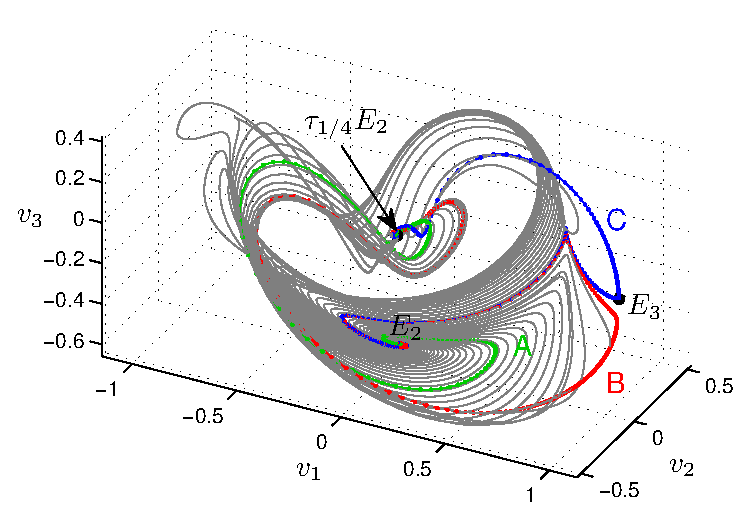
\includegraphics[width=0.48\textwidth]{figs/ks22_E2_manifold_c.eps}
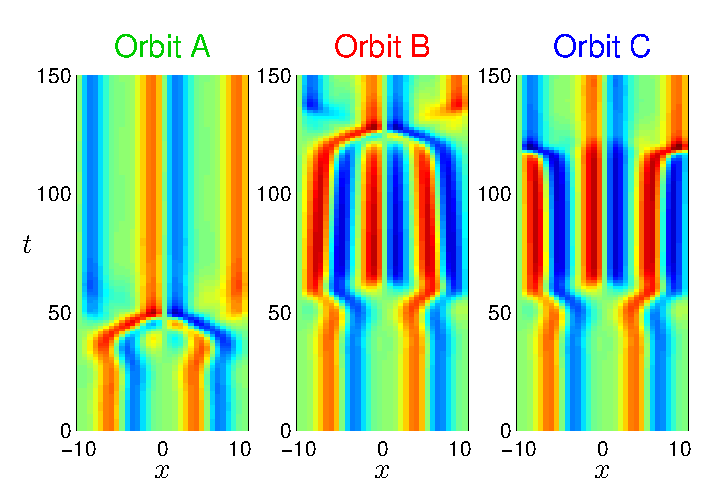
\includegraphics[width=0.48\textwidth]{figs/ks22_E2_orbits_c.eps}
\end{center}
\caption{
The left panel shows the two-dimensional
unstable manifold of \eqv\ \EQV{2}. The coordinate axes
$v_1$, $v_2$, and $v_3$ are constructed from vectors
\Re\, $\jEigvec{1}$, \Im\, $\jEigvec{1}$, and $\jEigvec{7}$
by Gram-Schmidt orthogonalization.
The right panel shows spatial representation of three orbits. Orbits
$B$ and $C$ pass close to the \eqv\ \EQV{3}. See
\reffig{f:KS22Manifold} for a different visualization.
       }
\label{f:KS22E2man}
\end{figure}


%%%%%%%%%%%%%%%%%%%%%%%%%%%%%%%%%%%%%%%%%%%%%%%%%%%%%%%%%%%%%%%%
\begin{figure}[t]
\begin{center}
%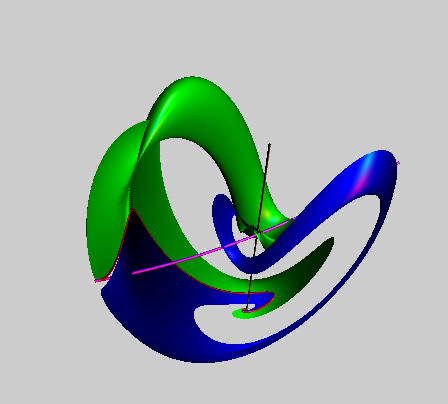
\includegraphics[width=0.6\textwidth]{figs/ks22manifold.ps}
(\textit{a}) 
\includegraphics[width=0.4\textwidth]{figs/ks22manifold1.eps}
(\textit{b}) 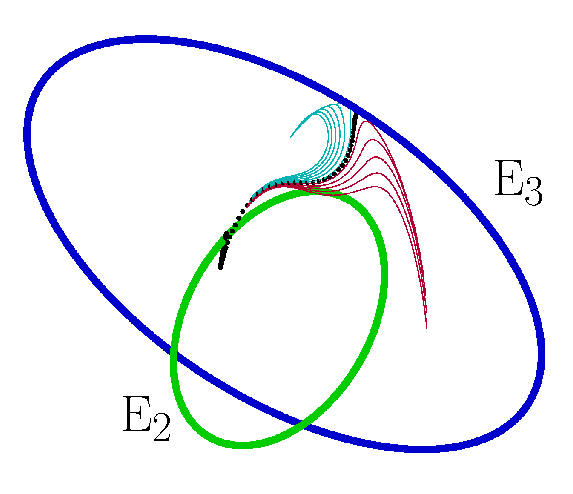
\includegraphics[width=0.4\textwidth]{figs/ks22E2-E3hetero.eps}
\end{center}
\caption{
(a) (blue/green) The unstable manifold of \EQV{2}~\eqv.
    (black line) The circle of \EQV{2}~\eqva\
related by the translation invariance.
(purple line) The circle  of \EQV{3}~\eqva.
(red) The heteroclinic connection
from the \EQV{2}~\eqv\ to the \EQV{3}~\eqv\ splits
the manifold into two parts,
colored (blue) and (green).  See
\reffig{f:KS22E2man} for a different visualization.
(b) \EQV{2}~\eqv\ to \EQV{3}~\eqv\ heteroclinic
connection. Here we omit the unstable manifold of \EQV{2},
keeping only a few neighboring trajectories in order to indicate
the unstable manifold of \EQV{3}. The \EQV{2} and \EQV{3}
families of \eqva\ arising from the continuous translational
symmetry of KS on a periodic domain are indicated by the two circles.
        }
\label{f:KS22Manifold}
\end{figure}
%%%%%%%%%%%%%%%%%%%%%%%%%%%%%%%%%%%%%%%%%%%%%%%%%%%%%%%%%%%%%%%%%%

The two-dimensional unstable manifold of \EQV{2} is shown in
\reffig{f:KS22E2man}.  All orbits within the manifold converge
to \EQV{2} shifted by $L/4$.  So this manifold can be viewed as a homoclinic
connection.  It also contains a pair of heteroclinic connections from
\EQV{2} to \EQV{3}.

The \eqv\ \EQV{3} has a pair of real unstable eigenvalues
equal to each other.  Therefore, within the plane spanned by the
corresponding eigenvectors, the orbits move radially away from
the \eqv.  In order to trace out the unstable manifold,
we start with a set of initial conditions within the unstable plane
\beq
 a(0) = a_{{\EQV{3}}} + \epsilon(v_1 \cos \phi + v_2 \sin \phi)\,,
  \quad\phi\in[0,2\pi]\,,
\label{unsManSeed}
\eeq
where $v_1$ and $v_2$ are orthonormal vectors within the
plane spanned by the two unstable eigenvectors, seeded as in
\refeq{linUnstMan}.
  The unstable manifold
of \EQV{3} is shown in \reffig{f:KS22E3man}.  The 3-fold symmetry of
the manifold is related to the symmetry of \EQV{3} with respect to
translation by $L/3$.  The manifold contains heteroclinic orbits
connecting \EQV{3} to three different points of the circle of {\eqva}
\EQV{2} translated set of solutions. Note also that the segments of orbits $B$ and $C$
between \EQV{3} and \EQV{2} in \reffigs{f:KS22E1man2}{f:KS22E2man}
represent the same heteroclinic connections as orbits $B$ and $C$ in
\reffig{f:KS22E3man}.

%%%%%%%%%%%%%%%%%%%%%%%%%%%%%%%%%%%%%%%%%%%%%%%%%%%%%%%%%%%%%%%%
\begin{figure}[t]
\begin{center}
\includegraphics[width=0.45\textwidth]{figs/ks22_E3_manifold.eps}
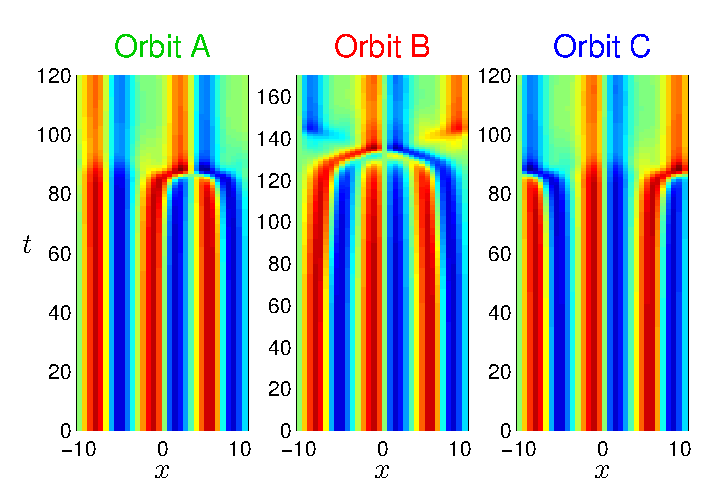
\includegraphics[width=0.5\textwidth]{figs/ks22_E3_orbits_c.eps}
\end{center}
\caption{
The left panel shows the two-dimensional
unstable manifold of \eqv\ \EQV{3}. The coordinate axes
$v_1$, $v_2$, and $v_3$ are constructed from vectors
$\jEigvec{1}$, $\jEigvec{2}$, and $\jEigvec{4}$ by Gram-Schmidt orthogonalization.
The black line shows a family of \EQV{2}~\eqva\ related by translational
symmetry. The right panel shows spatial representation of
three orbits. Orbits $B$ and $C$ are two different heteroclinic orbits
connecting \EQV{3} to the same point on the \EQV{2} line.
        }
\label{f:KS22E3man}
\end{figure}
%%%%%%%%%%%%%%%%%%%%%%%%%%%%%%%%%%%%%%%%%%%%%%%%%%%%%%%%%%%%%%%%

An understanding of the ubiquity of heteroclinic connections in KSe, as
opposed to their non-genericity in a general high-dimensional system, is provided in \refref{KNSks90}.
For our system size
there are exactly two representatives
of the $\EQV{2}$ family that lie in the intersection of $\bbU^+$ and $\bbU^{(1)}$ related
to each other by an $L/4$ shift. Denote them by $\EQV{2}$ and $\Shift_{1/4}\EQV{2}$ respectively. The unstable eigenplane of
$\EQV{2}$ lies on $\bbU^+$ while that of $\Shift_{1/4}\EQV{2}$ lies on $\bbU^{(1)}$, \cf\ \reftab{tab:Eksym}.
The $\EQV{3}$ family members that live in $\bbU^+$ have one of their unstable eigenvectors (the one related to the heteroclinic
connection to $\EQV{2}$ family)  on $\bbU^+$, while the other does not lie on symmetry-invariant subspace.
Similarly, for the $\EQV{1}$ family we observe that the equilibria in $\bbU^+$ have
an unstable plane on $\bbU^+$ (again related to the heteroclinic connection) and a second one with no symmetry.
Thus $\Shift_{1/4}\EQV{2}$ appears as a sink on $\bbU^+$, while all other equilibria appear as sources.
This explains the heteroclinic connections from $\EQV{1}\,,\EQV{2}$ and $\EQV{3}$ to $\Shift_{1/4}\EQV{2}$.
Observing that $\Shift_{1/4} \bbU^+= \bbU^{(1)}$ and taking into account \reftab{tab:Eksym} we understand that within $\bbU^{(1)}$
we have connections from $\Shift_{1/4}\EQV{2}$ (and members of $\EQV{1}$ and $\EQV{3}$ families) to $\EQV{2}$ and the
formation of a heteroclinic loop. Due to the translational invariance of KS there is a heteroclinic loop for any two points
of the $\EQV{2}$ family related by an $L/4$-shift.

%%%%%%%%%%%%%%%%%%%%%%%%%%%%%%%%%%%%%%%%%%%%%%%%%%%%%%%%%%%%%%%%
\begin{figure}[t]
\begin{center}
        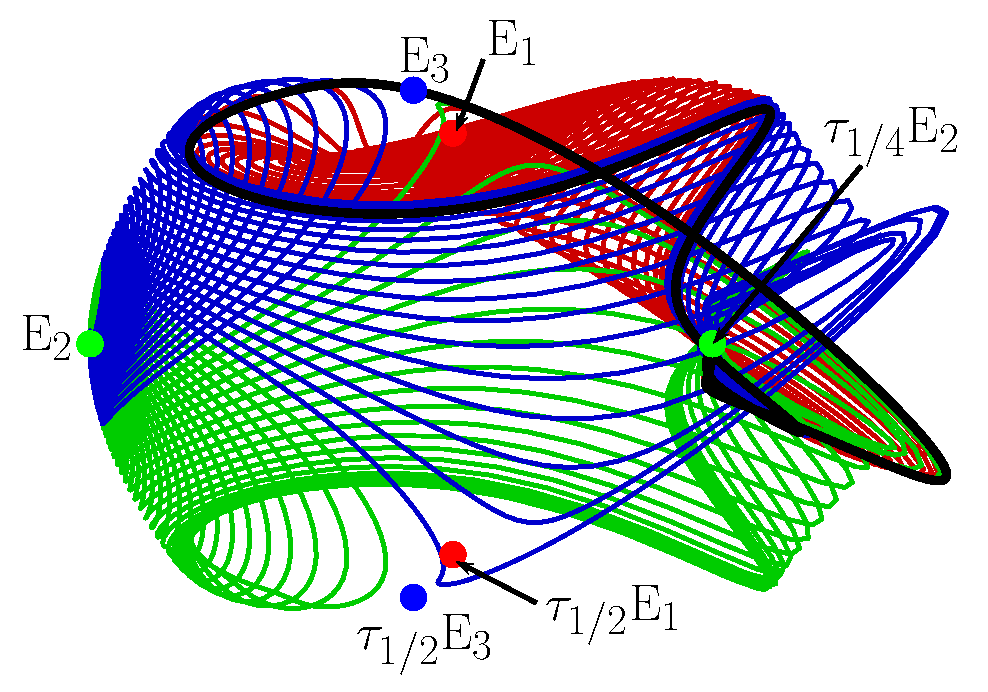
\includegraphics[width=0.6\textwidth]{figs/KS22hetero.eps}
\end{center}
\caption{ Heteroclinic connections on $\bbU^+$:
 (red) The unstable manifold of \EQV{1}~\eqv.
 (blue/green) The unstable manifold of \EQV{2}~\eqv.
 (black) Heteroclinic connections from \EQV{3}~\eqv to $\Shift_{1/4}$\EQV{2}~\eqv.
 The unstable manifolds of $\Shift_{1/2}$\EQV{1} and $\Shift_{1/2}$\EQV{2} have been ommited
 for clarity. Projection from $128$ dimensions onto the plane given by the vectors
 $\EQV{2}-\Shift_{1/4}\EQV{2}$ and $\EQV{3}-\Shift_{1/2}\EQV{3}$.}
\label{f:KS22hetero}
\end{figure}
%%%%%%%%%%%%%%%%%%%%%%%%%%%%%%%%%%%%%%%%%%%%%%%%%%%%%%%%%%%%%%%%%%

\section{\Rpo s for $L=22$}
\label{sec:rpos}

The \rpo s satisfy the condition \refeq{KSrpos}
$u(x+\shift_p,\period{p}) = u(x,0)$,
where $\period{p}$ is the period and $\shift_p$ the phase shift.
We have limited our search to orbits with $\period{p} < 200$ and found
over 300 \rpo s with $\shift_p > 0$.
Each \rpo\ with phase shift
$\shift_p \neq 0$ has a reflection symmetric partner
$u_p(x) \to -u_p(-x)$ with phase shift $-\shift_p$.

The search has not been exhaustive, and there are likely to be more
orbits with $\period{p} < 200$. However, the orbits we have found provide a representative sample of
typical periodic and \rpo s and approximate well the chaotic
attractor (since they were located using seeds obtained from close
returns within the chaotic dynamics).

\begin{figure}[t]
\begin{center}
(\textit{a})\hspace{1ex}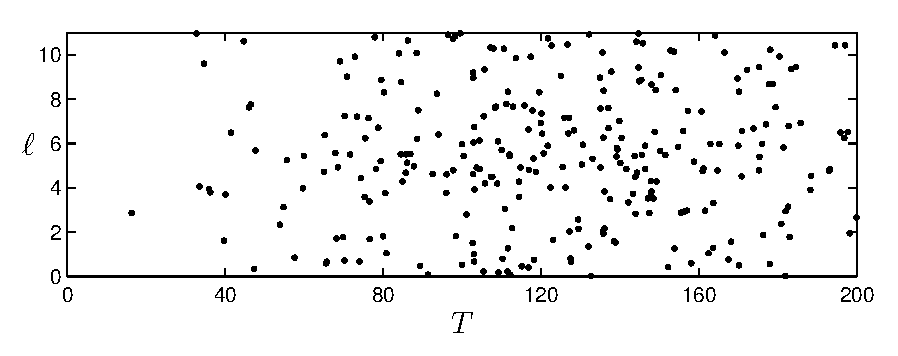
\includegraphics[width=0.7\textwidth]{figs/ks22_rpos_Tdelta.eps}\\
(\textit{b})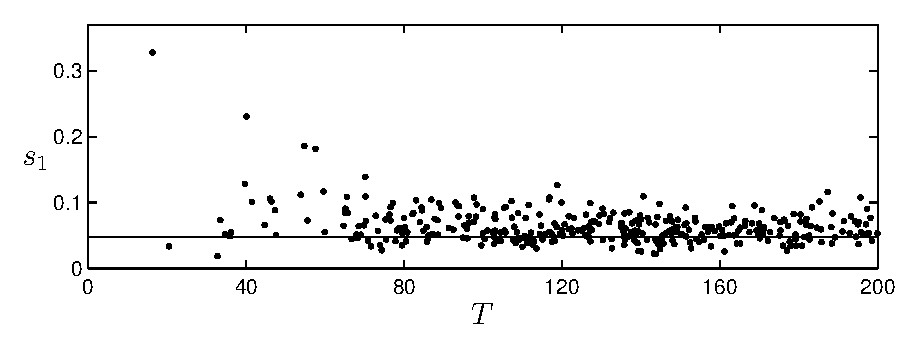
\includegraphics[width=0.72\textwidth]{figs/ks22_rpos_lyap.eps}
\end{center}
\caption{
(a) All \rpo s of \KSe\ determined here, with periods $\period{p}$ and
shifts $\shift_p > 0$.
(b) The largest Lyapunov exponents \refeq{FloqExp} of all
\rpo s and pre-periodic orbits with reflection.
The horizontal line at $0.048$
indicates the numerical value  of the largest
Lyapunov exponent of the chaotic attractor.
} \label{f:ks22rposT}
\end{figure}

\refFig{f:ks22rposT}\,(\textit{a}) shows the \rpo s in the plane
$(\period{},\shift)$.  Not much is learned from such plot other than
that for longer periods the \rpo s are scattered over the
whole $(\period{},\shift)$ plane.

The stability of the orbits is determined by their Lyapunov exponents,
defined as
\beq
	s_j = \eigRe[j]/\period{p} \,,
\ee{FloqExp}
where $\ExpaEig_j = e^{\eigRe[j] \pm i \eigIm[j]}$ are the
eigenvalues of the fundamental matrix $\mathbf{g}(\shift_p)J(a_p,\period{p})$
(see Appendix~\ref{sec:stability}).

As was already the case for the Lyapunov exponents
discussed in \refSect{sec:L22}, for all
periodic and \rpo s we have found, only four Lyapunov
exponents are dynamically relevant, with the remaining ones indicating
strong contraction towards the 4-dimensional manifold containing the chaotic attractor.
Out of the four leading exponents, two equal zero, due to
the time and space translational invariance of the orbits.  Of the
remaining two, one is always positive, while the second one is
either positive or negative.

The scatter of the largest Lyapunov exponents
of periodic and \rpo s is shown in \reffig{f:ks22rposT}\,(\textit{b}).
In this case some tendency of accumulation toward the largest
Lyapunov exponent 0.048 of the chaotic attractor
can be noted.  This, however, is in part an artifact of initializing
the \rpo\ searches by near recurrences in long-time \statesp\
trajectories.

The small period \rpo s outline the coarse structure of the chaotic
attractor, while the longer period \rpo s resolve the finer details
of the dynamics.
The first four orbits with the shortest periods we have found are
shown in \reffig{f:ks22rpos}(\textit{a-d}).  The shortest orbit with
$\period{p} = 16.4$ is also the most unstable, with one positive
Lyapunov exponent equal 0.328.  The other short orbits are less
unstable, with the largest Lyapunov exponent 
in the range
0.018 -- 0.073, typical of the long time attractor average.

%%%%%%%%%%%%%%%%%%%%%%%%%%%%%%%%%%%%%%%%%%%%%%%%%%%%%%%%%%%%%%%%
\begin{figure}[t]
\begin{center}
\begin{tabular}{cccccc} (\textit{a}) & (\textit{c}) & (\textit{e}) &
                        (\textit{g}) & (\textit{i}) & (\textit{k})\\
\includegraphics[width=0.15\textwidth]{figs/ks22rpo016.3-02.86.eps}\hspace{-3ex} &
\includegraphics[width=0.15\textwidth]{figs/ks22rpo033.5-04.04.eps}\hspace{-3ex} &
\includegraphics[width=0.15\textwidth]{figs/ks22rpo047.6-05.68.eps}\hspace{-3ex} &
\includegraphics[width=0.15\textwidth]{figs/ks22rpo071.7-05.50.eps}\hspace{-3ex} &
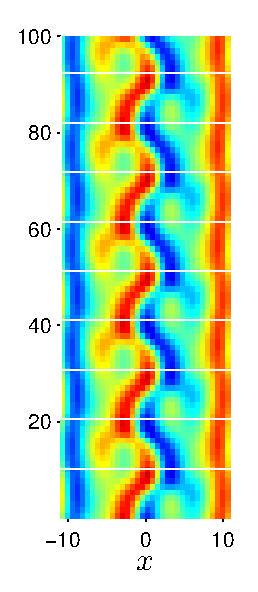
\includegraphics[width=0.15\textwidth]{figs/ks22rpo020.5-00.00.eps}\hspace{-3ex} &
\includegraphics[width=0.15\textwidth]{figs/ks22rpo066.8-00.00.eps}\\
(\textit{b}) & (\textit{d}) & (\textit{f}) &
(\textit{h}) & (\textit{j}) & (\textit{l})\\
\includegraphics[width=0.15\textwidth]{figs/ks22rpo032.8-10.96.eps}\hspace{-3ex} &
\includegraphics[width=0.15\textwidth]{figs/ks22rpo034.6-09.60.eps}\hspace{-3ex} &
\includegraphics[width=0.15\textwidth]{figs/ks22rpo059.9-05.44.eps}\hspace{-3ex} &
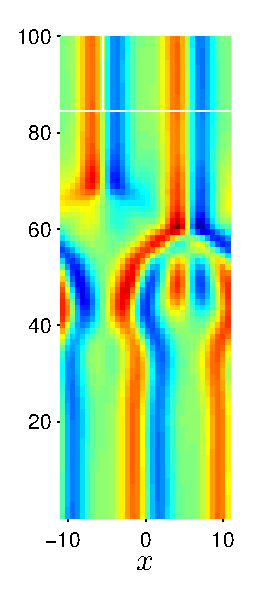
\includegraphics[width=0.15\textwidth]{figs/ks22rpo084.4-05.51.eps}\hspace{-3ex} &
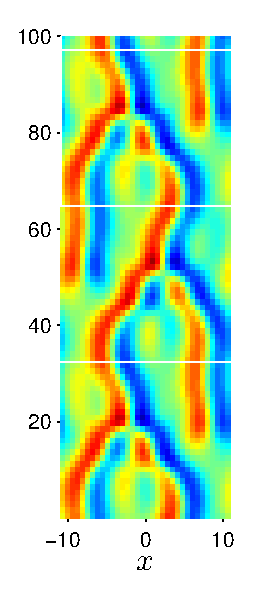
\includegraphics[width=0.15\textwidth]{figs/ks22rpo064.7-00.00.eps}\hspace{-3ex} &
\includegraphics[width=0.15\textwidth]{figs/ks22rpo070.3-00.00.eps}
\end{tabular}
\end{center}
\caption{Selected relative periodic and
pre-periodic
orbits of \KSe\ with $L = 22$:
(a) $\period{p} = 16.3$, $\shift_p = 2.86$;
(b) $\period{p} = 32.8$, $\shift_p = 10.96$;
(c) $\period{p} = 33.5$, $\shift_p = 4.04$;
(d) $\period{p} = 34.6$, $\shift_p = 9.60$;
(e) $\period{p} = 47.6$, $\shift_p = 5.68$;
(f) $\period{p} = 59.9$, $\shift_p = 5.44$;
(g) $\period{p} = 71.7$, $\shift_p = 5.503$;
(h) $\period{p} = 84.4$, $\shift_p = 5.513$;
(i) $\period{p} = 10.3$;
(j) $\period{p} = 32.4$;
(k) $\period{p} = 33.4$;
(l) $\period{p} = 35.2$.
Horizontal and vertical white lines indicate periodicity and phase
shift of the orbits, respectively.
}\label{f:ks22rpos}
\end{figure}
%%%%%%%%%%%%%%%%%%%%%%%%%%%%%%%%%%%%%%%%%%%%%%%%%%%%%%%%%%%%%%%%


We have found \rpo s which stay
close to the unstable manifold of \EQV{2}.
As is illustrated in \reffig{f:ks22rpos}(\textit{e-h}), all such orbits have
shift $\shift_p \approx L/4$, similar to the shift of orbits within
the unstable manifold of \EQV{2}, which start at \EQV{2} and
converge to $\Shift_{1/4}$\EQV{2} (see \reffig{f:KS22E2man}). This
confirms that the `cage' of unstable manifolds of equilibria plays
an important role in organizing the chaotic dynamics of the \KS\
equation.


\section{Pre-periodic orbits} \label{ssec:po}

As discussed in \refSect{sec:KSePO}, a \rpo\ will be periodic, \ie,
$\shift_p = 0$, if it either {\bf (a)} lives within the $\bbU^+$ antisymmetric
subspace, $-u(-x,0) = u(x,0)$, or {\bf (b)}
returns to its reflection
after a period: $u(x,\period{p})=-u(-x,0)$,
and is thus periodic
with period $2\period{p}$.
The dynamics of
\KSe\ in the antisymmetric subspace and \po s with symmetry {\bf (a)} have
been investigated
previously\rf{Christiansen97,LanThesis,LanCvi07}. The KS equation
with $L = 22$ does not have any periodic orbits of this type.

We have found over 50
pre-periodic orbits with $\period{p} < 100$
which possess the symmetry
of type {\bf (b)}. Some of the shortest such orbits we have found are shown in
\reffig{f:ks22rpos}(\textit{i-l}).
Several were found as
repeats of pre-periodic orbits during searches
for \rpo s with non-zero shifts,
while most have been
found as solutions of the pre-periodic orbit
condition \refeq{KSpos} with reflection,
which takes form
\beq
 -\mathbf{g}(-\shift)a^\ast(\period{p}) = a(0)\,.
\label{KSposFour}
\eeq
in the Fourier space representation
(compare it to the condition \refeq{eq:system} for \rpo s).


\section{Energy transfer rates}
\label{sec:energyL22}


%%%%%%%%%%%%%%%%%%%%%%%%%%%%%%%%%%%%%%%%%%%%%%%%%%%%%%%%%%%%%%%%
\begin{figure}[t]
\begin{center}
 \begin{tabular}{cc}
		~~~~~~~~(\textit{a})						&	~~~~~~~~(\textit{b}) \\
 	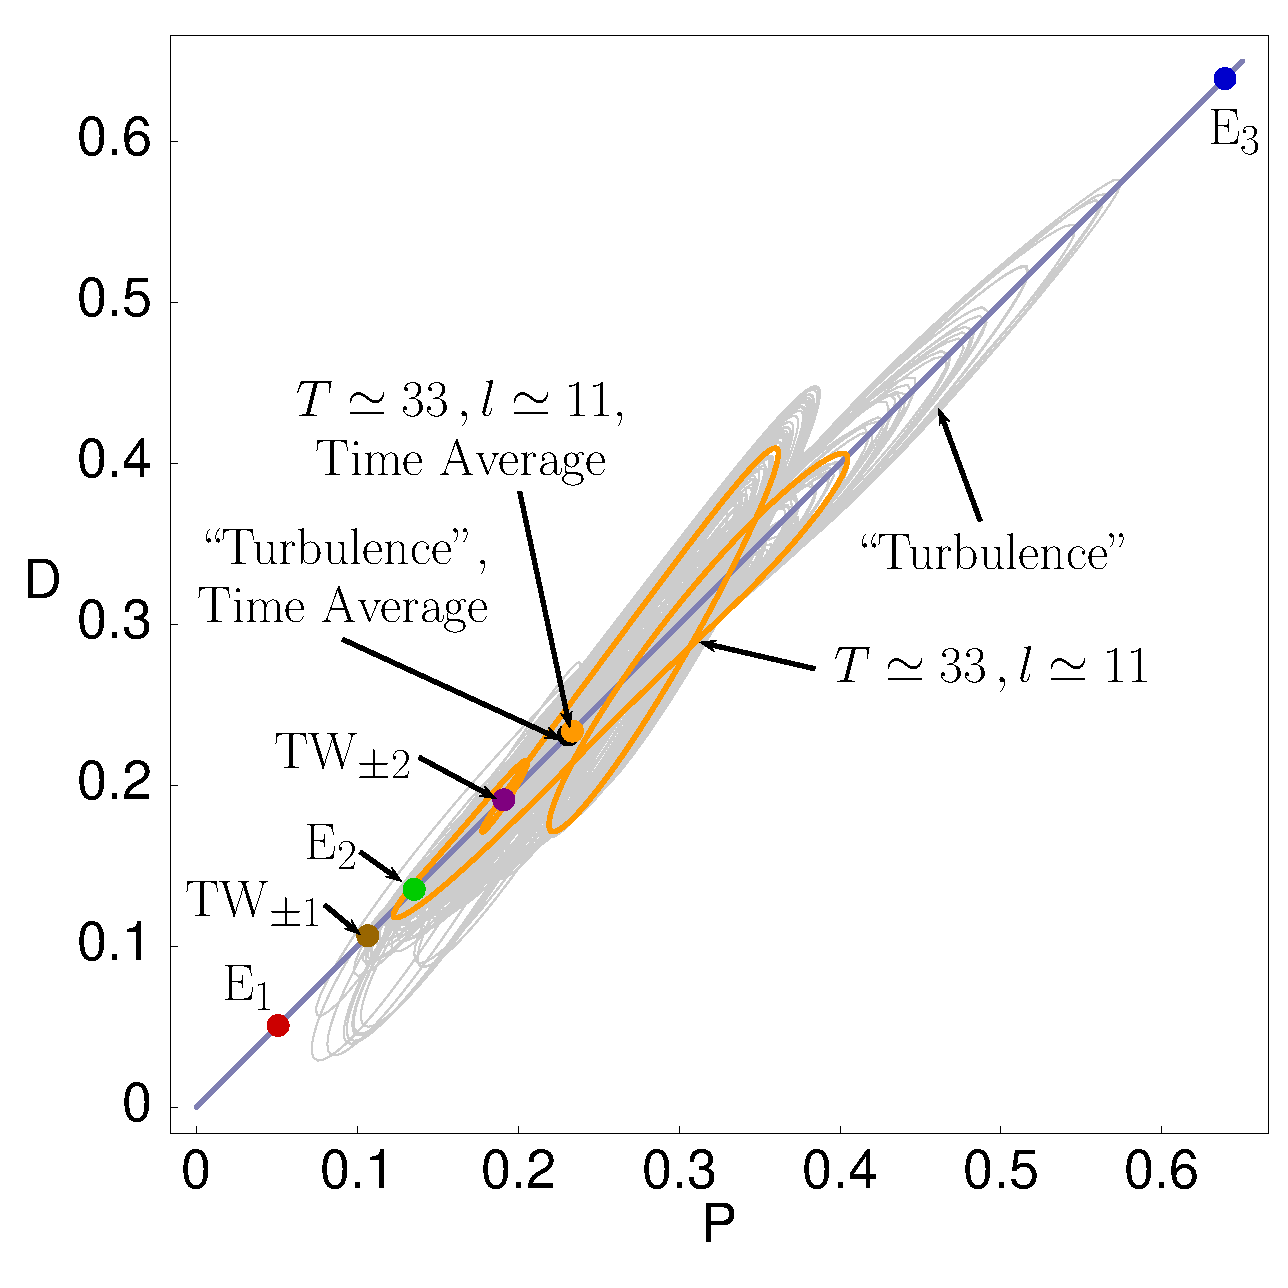
\includegraphics[width=0.46\textwidth]{figs/energyBalance_pst.eps} 	& 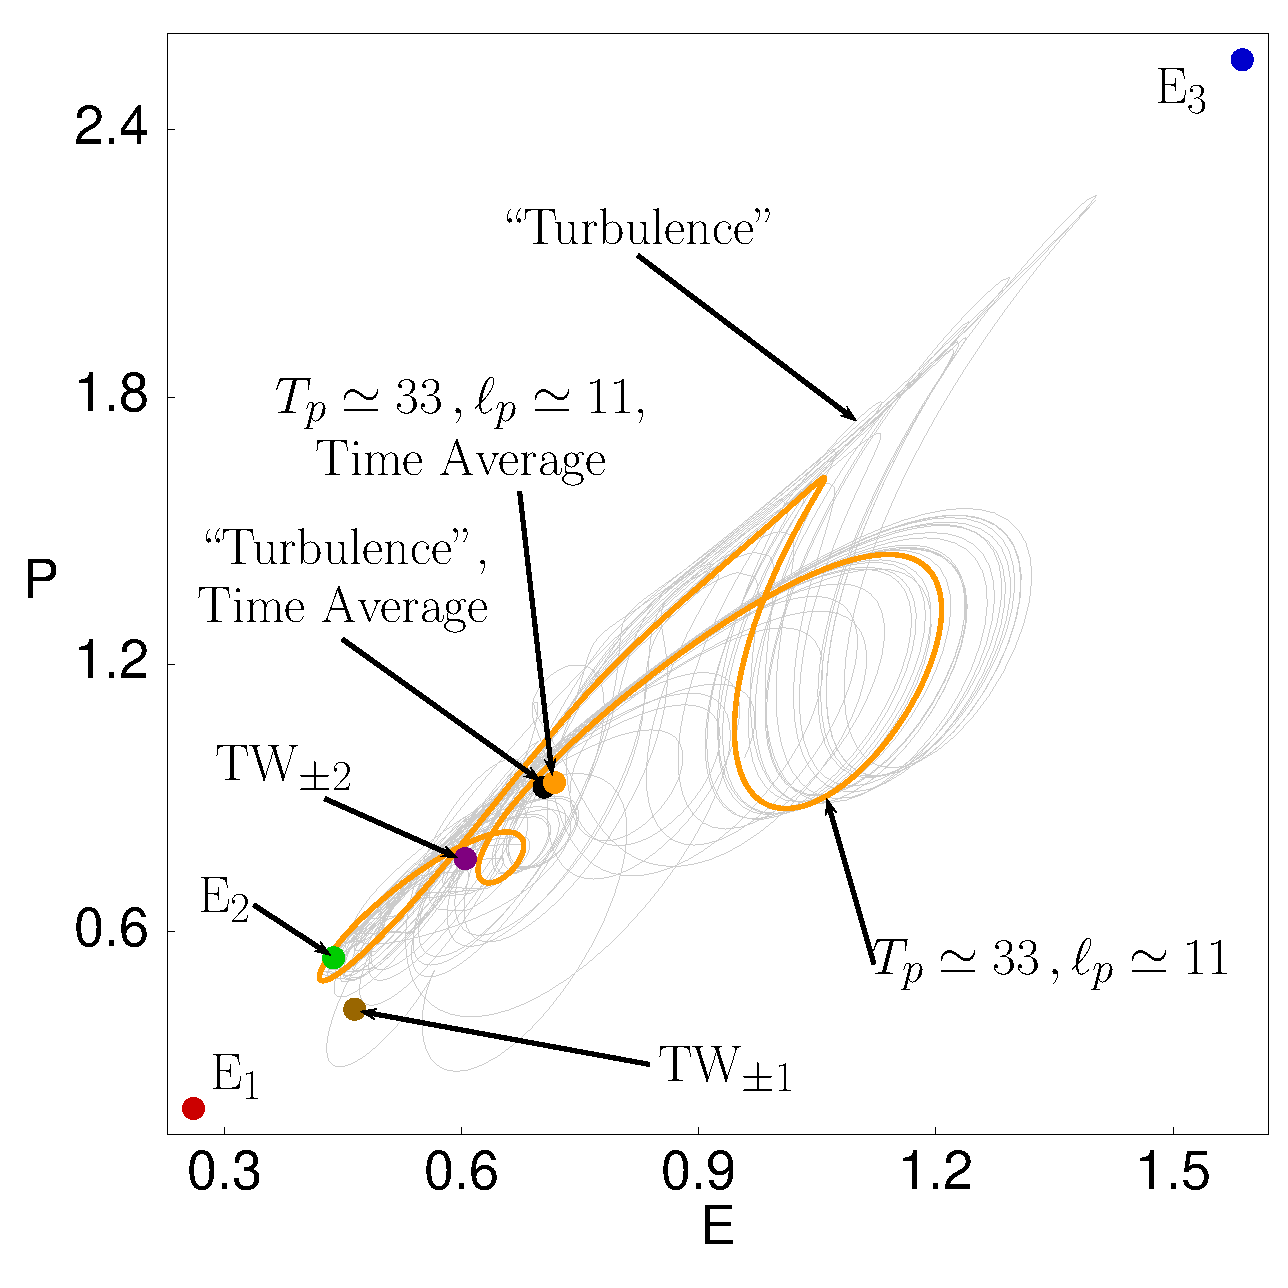
\includegraphics[width=0.46\textwidth]{figs/equivaEP_pst.eps}

  \end{tabular}
\end{center}
\caption{
(a) Power input $P$ {\em vs.}
dissipation rate $D$
(b) energy $E$  {\em vs.}
power input $P$,   for several  \eqva\ and \reqva,
a \rpo , and a typical `turbulent' long-time trajectory.
System size $L=22$.
        }
\label{f:drivedrag}
\end{figure}
%%%%%%%%%%%%%%%%%%%%%%%%%%%%%%%%%%%%%%%%%%%%%%%%%%%%%%%%%%%%%%%%%%

%%%%%%%%%%%%%%%%%%%%%%%%%%%%%%%%%%%%%%%%%%%%%%%%%%%%%%%%%%%%%%%%
\begin{figure}[t]
\begin{center}
 \begin{tabular}{cc}
		~~~~~~~~(\textit{a})						&	~~~~~~~~(\textit{b}) \\
	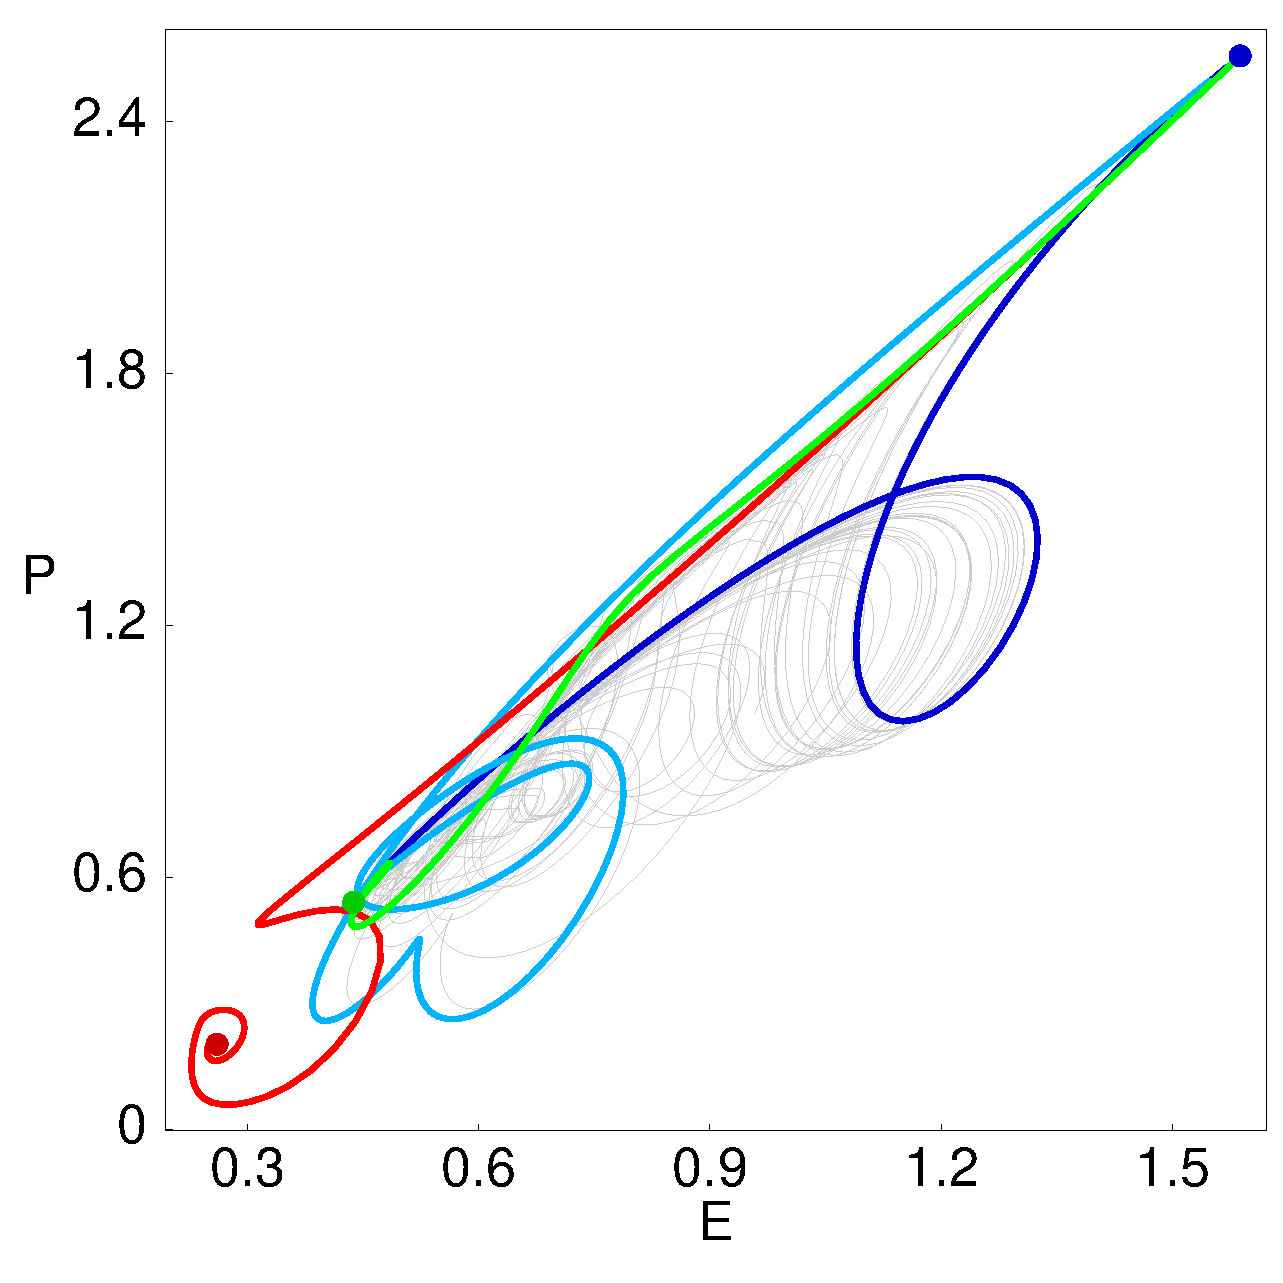
\includegraphics[width=0.46\textwidth]{figs/connEP.eps}		& 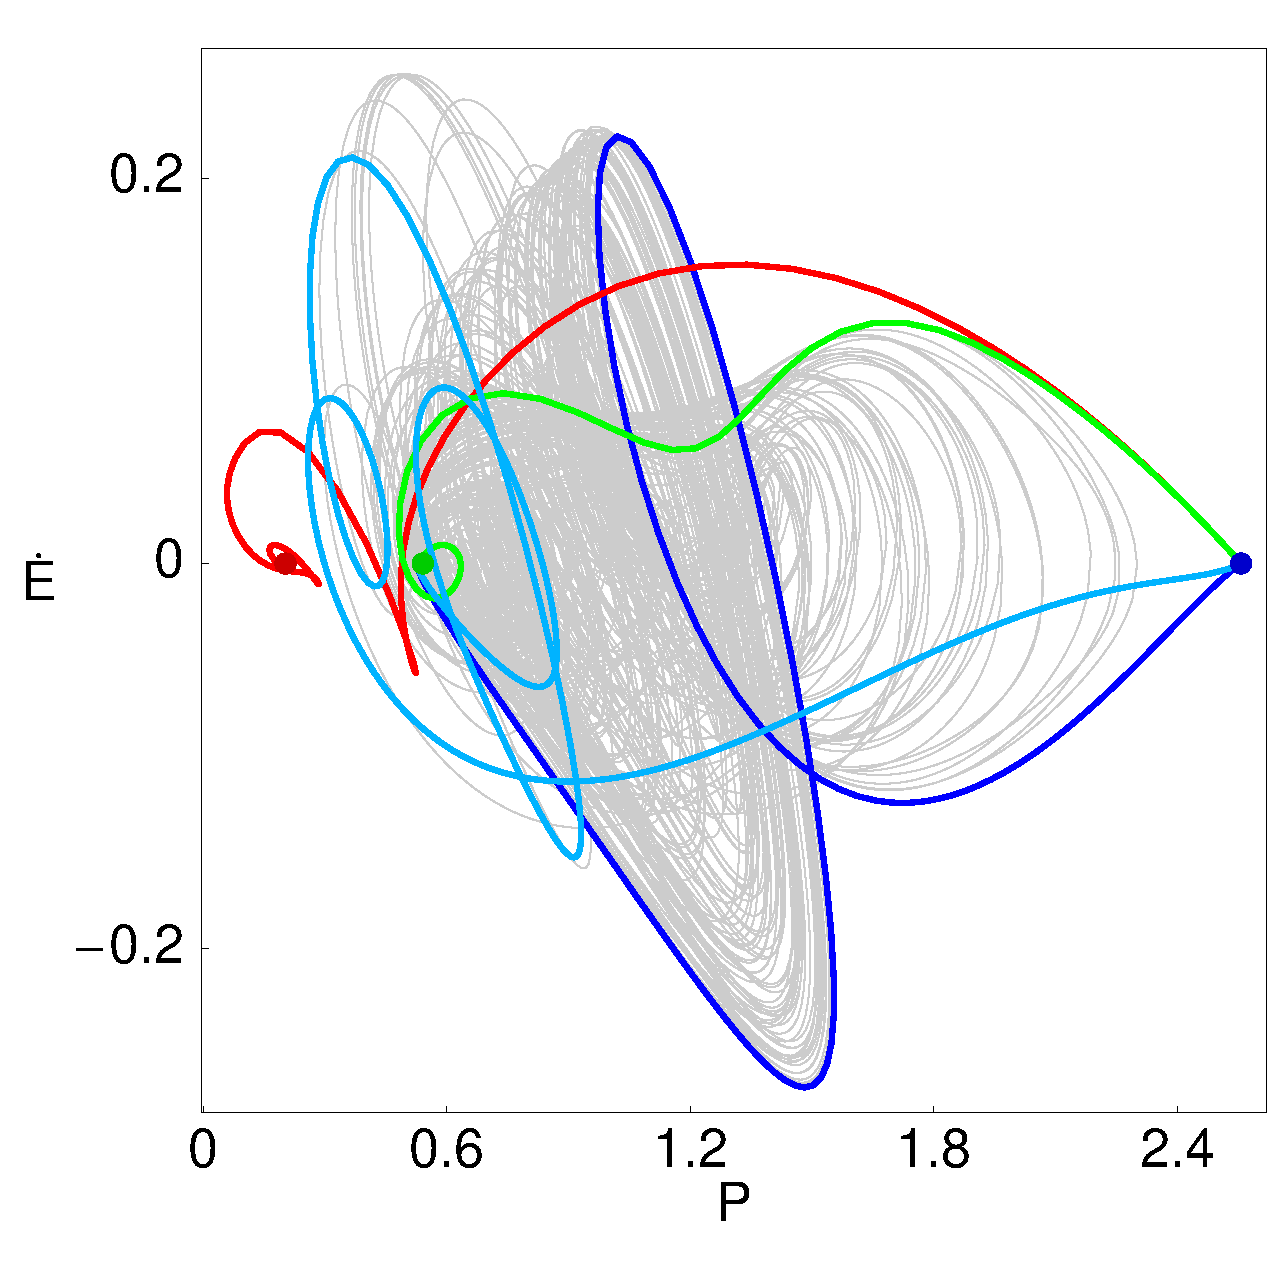
\includegraphics[width=0.46\textwidth]{figs/connPEdot.eps}
 \end{tabular}
\end{center}
\caption{
Two projections of the $(E,P,\dot{E})$ representation of the flow.
\EQV{1} (red), \EQV{2} (green), \EQV{3} (blue),
heteroclinic connections from \EQV{2} to $\EQV{3}$ (green),
from $\EQV{1}$ to \EQV{3} (red)
and from \EQV{3} to $\EQV{2}$ (shades of blue), superimposed over
a generic long-time `turbulent' trajectory (grey).
System size $L=22$.
        }
\label{f:drivedragConn}
\end{figure}
%%%%%%%%%%%%%%%%%%%%%%%%%%%%%%%%%%%%%%%%%%%%%%%%%%%%%%%%%%%%%%%%%%

In \reffig{f:drivedrag} we plot \refeq{EnRate}, the time-dependent
$\dot{\expctE}$ in the power input $P$ {\em vs.}
dissipation rate $D$ plane, for $L=22$ \eqva\ and \reqva,
a selected \rpo, and for a typical `turbulent' long-time
trajectory.

Projections from the $\infty$-dimensional \statesp\ onto the 3-dimensional
$(E,P,D)$ representation of the flow, such as
\reffigs{f:drivedrag}{f:drivedragConn}, can be misleading.
The most one can say is that if points are clearly separated in an
$(E,P,D)$ plot (for example, in \reffig{f:drivedrag}
$\EQV{1}$ \eqv\ is outside the recurrent set), they are also separated
in the full \statesp.  Converse is not true -- states of
very different topology can have similar energies.

An example is
the \rpo\ $(\period{p},\shift_p) = (32.8,10.96)$
(see \reffig{f:ks22rpos}(\textit{b})) which appears well embedded
within the turbulent flow. The mean power $\timeAver{P_p}$ evaluated
as in \refeq{poE}, see \reffig{f:drivedrag},
is numerically quite close to the long-time
turbulent time average $\timeAver{P}$.
Similarly close prediction of mean dissipation rate in the
\pCf\ from a single-period \po\ computed by
Kawahara and Kida\rf{KawKida01} has lead to
optimistic hopes that `turbulence' is different from
low-dimensional chaos, insofar that the determination of one special
\po\ could yield all long-time averages.
Regrettably, not true -- as always, here too one needs a hierarchy
of \po s of increasing length to obtain accurate
predictions\rf{DasBuch}.

%%%%%%%%%%%%%%%%%%%%%%%%%%%%%%%%%%%%%%%%%%%%%%%%%%%%%%%%%%%%%%%%
\begin{figure}[t]
\begin{center}
(\textit{a})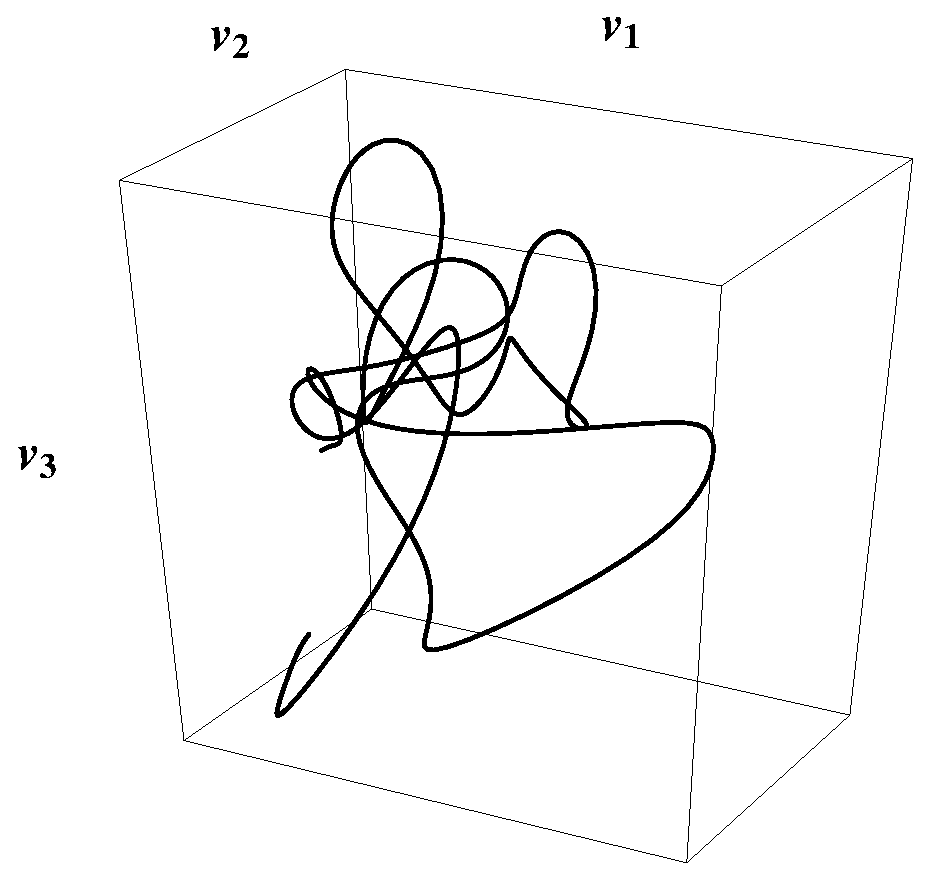
\includegraphics[width=0.46\textwidth]{figs/ks22rpo033.50_04.045E2.eps}
(\textit{b})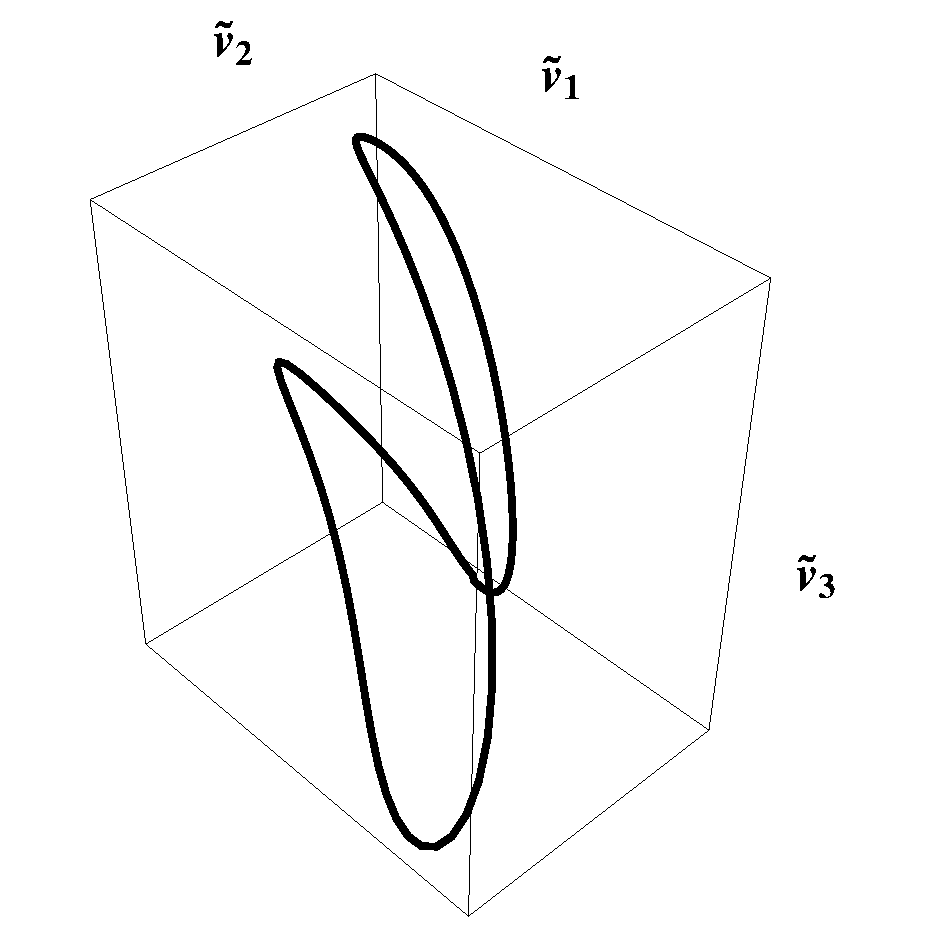
\includegraphics[width=0.46\textwidth]{figs/ks22rpo033.50_04.045E2CM.eps}
\\
\end{center}
\caption{
 The
\rpo\ with $(\period{p},\shift_p) =(33.5,4.04)$
from \reffig{f:ks22rpos}\,(\textit{c})
which appears well embedded within the turbulent flow:
 (a) A stationary \statesp\ projection,
  traced for four periods $\period{p}$. The coordinate axes
$v_1$, $v_2$, and $v_3$ are those of \reffig{f:KS22E2man};
 (b) In the co-moving mean velocity frame,
 traced for one period $\period{p}$.
        } \label{f:MeanVelocityFrame}
\end{figure}
%%%%%%%%%%%%%%%%%%%%%%%%%%%%%%%%%%%%%%%%%%%%%%%%%%%%%%%%%%%%%%%%%%

For any given \rpo\ a convenient visualization is
offered by the {\em mean velocity frame}, {\ie},
a reference frame that rotates with velocity
$v_p=\shift_p/\period{p}$.
In the mean velocity frame a \rpo\ becomes
a \po, as in \reffig{f:MeanVelocityFrame}\,(\textit{b}).
However, each {\rpo} has its own mean velocity frame and thus
sets of \rpo s are difficult to visualize simultaneously.


% relativeKS.tex
% copied here from nsf/nsf06am/TEX/relativeKS.tex 		Nov 1 2006
% $Author: gibson $ $Date: 2006-10-31 13:29:59 -0500 (Tue, 31 Oct 2006) $



The KS work
% described in \refsect{s:KS}
of \refref{Christiansen:97}
was restricted to the antisymmetric subspace.
The restriction to antisymmetric subspace was used
to eliminate the continous translational symmetry of \KSe.
Due to the lack of self-adjointness
(non-normality) of the linearized \KS\ flow, 
the antisymmetric subspace
is unstable under small perturbations, and generic solutions of 
KS belong to the full, periodic space.
Nevertheless, 
the \eqva\ and the shortest \po s orbits that lie in this subspace
and play important role for global topology of the flow,
together
with the \reqva\ and \rpo s
characteristic of the full, continuous translation invariant space..
The key new feature of the full, periodic domain
KS is its continous translational symmetry,
with attendandt continuous families of
\reqva\ (travelling waves) and \rpo s.
\Rpo s, in particular, require rethinking dynamical systems
approach to constructing symbolic dynamics. 

%%%%%%%%%%%%%%%%%%%%%%%%%%%%%%%%%%%%%%%%%%%%%%%%%%%%%%%%%%%%%%%%
\begin{figure}[h]\vspace*{-5pt}
\centering
(a)\includegraphics[width=0.17\textwidth]%,origin=c]
                {figs/kse22_E1_chaos_color.eps}
~~~
(b)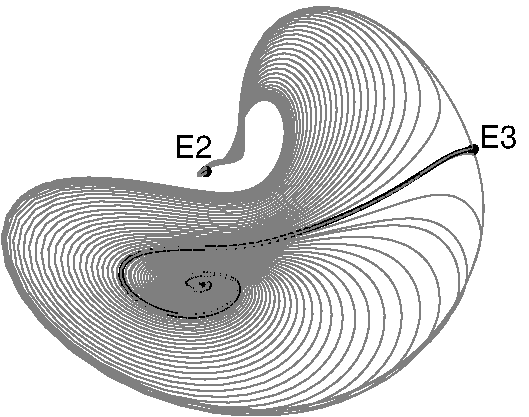
\includegraphics[width=0.33\textwidth]{figs/kse22_E1_UM2.eps}
(c)\includegraphics[width=0.3\textwidth]%,origin=c]%
        {figs/ks22E2-E3hetero.ps}
\vspace*{-5pt}\caption{
{\small
(a) A perturbed unstable \nameit{1}~\eqv\ and its decay
    into a typical turbulent state.
(b) \nameit{1}~\eqv\ unstable manifold, 
    with the trajectory connecting the
\nameit{2}~\eqv\ point to the unique corresponding heteroclinic
point in the \nameit{3}~\eqv\ family. \nameit{3}
unstable manifold in turn connects \nameit{3} to the
stable manifold of \nameit{2}.
(c) \nameit{2}~\eqv\ to \nameit{3}~\eqv\ heteroclinic 
connection. Here we omit the unstable manifold of \nameit{2},
keeping only a few neighboring trajectories in order to indicate
the unstable manifold of \nameit{3}, and show the \nameit{2} and \nameit{3}
families of \eqva\ arising from the continuous translational
symmetry of KS on a periodic domain. 
% separatrix.
$\tilde{L}=3.5014$, 2$d$ projections from 64 
complex Fourier modes phase space.
        } %end \small
        }
\label{f:KS22unstM}\vspace*{-5pt}
\end{figure}
%%%%%%%%%%%%%%%%%%%%%%%%%%%%%%%%%%%%%%%%%%%%%%%%%%%%%%%%%%%%%%%%%%
\PC{a bit of a cheat - \reffig{f:KS22unstM}\vspace*{-5pt} has
    2 unstable complex-pair planes}


%%%%%%%%%%%%%%%%%%%%%%%%%%%%%%%%%%%%%%%%%%%%%%%%%%%%%%%%%%%%%%%%
\begin{figure}[h]\vspace*{-5pt}
\centering
(a)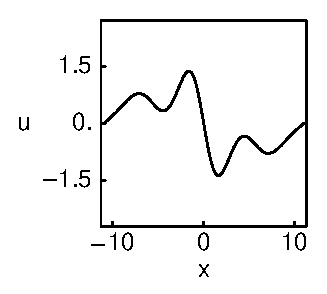
\includegraphics[width=0.25\textwidth]{figs/1wKS22equil.eps}
(b)\includegraphics[width=0.25\textwidth]%,origin=c]
                {figs/2wKS22equil.eps}
(c)\includegraphics[width=0.25\textwidth]%,origin=c]%
        {figs/3wKS22equil.eps}
\vspace*{-5pt}\caption{
{\small
(a) \nameit{1}eqv,
(b) \nameit{2} and
(c) \nameit{3}~\eqva. $\tilde{L}=3.5014$, N=64 mode truncation.
        } %end \small
        }
\label{f:KS22Equil}\vspace*{-5pt}
\end{figure}
%%%%%%%%%%%%%%%%%%%%%%%%%%%%%%%%%%%%%%%%%%%%%%%%%%%%%%%%%%%%%%%%%%

An instructive 
example is offered by the dynamics for $\tilde{L}=3.5014$, % (L=22).
currently studied in collaboration with
R.L. Davidchack (U. Leicester, UK).
For this small periodic cell
the chaotic dynamics arises from
a competition between unstable
wavelength 2- and 3- coherent structures.
We refer to wavelength 1-, 2- and 3- unstable \eqva\ as
\nameit{1},\nameit{2} and \nameit{3},
respectively.
In \reffig{f:KS22unstM} (a)
color indicates the value of $u(x,t)$ in 
the $(x,t)$ space-time plane.
Spatial representations of
PDEs (such as the 3$d$
snapshots of velocity and vorticity fields in Navier-Stokes)
offer little insight into detailed dynamics of low-$Re$ flows.
Much more illuminating are the phase space representations.
In \refFig{f:KS22unstM} (b) the \eqv\ \nameit{1} of
\reffig{f:KS22unstM} (a) is represented by the point \nameit{1},
and its unstable manifold can be examined in great detail.
To each \eqv\ point corresponds a continous family
of \eqva, and this leads to an unexpected feature of such
flows: While in dimensions higher than 2 heteroclinic connections 
are a rarity (likelihood that unstable manifold of one
 \eqv\ precisely hits another \eqv\ point is zero), 
for flows with continuous symmetries intersections of unstable
manifolds with continuous families of equvalent \eqva\ are common.
\refFig{f:KS22unstM} (b) and (c) show 
such heteroclinic connections.
% from an \nameit{2}~\eqv\ point to \nameit{3}~\eqv\ family.
These connections partition the phase space,
and will be the basis of our
{\bf construction of symbolic dynamics}.
Effective symbolic dynamics allows
for a systematic and exhaustive determination 
of all \rpo s, in the spirit of 
the earlier work presented in \refsect{s:KS}.
Many short unstable \rpo s have been already 
been computed using trial trajectories based on above
topological connections as starting  guesses 
for variants of the Newton method.
% They typically have either one unstable eigenvalue, or one complex
% eigenvalue pair.

KS symbolic dynamics will
serve as a testbed for developing the
same for PCF, and for applications of the new
trace formula with continous symmetries (\refsect{s:relativePOT}).

%%%%%%%%%%%%%%%%%%%%%%%%%%%%%%%%%%%%%%%%%%%%%%%%%%%%%%%%%%%%%%%%
\begin{figure}[h]\vspace*{-5pt}
\centering
%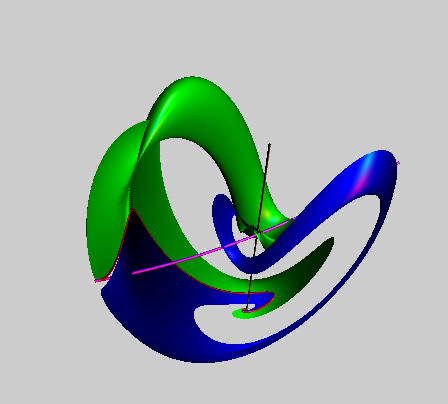
\includegraphics[width=0.6\textwidth]{figs/ks22manifold.ps}
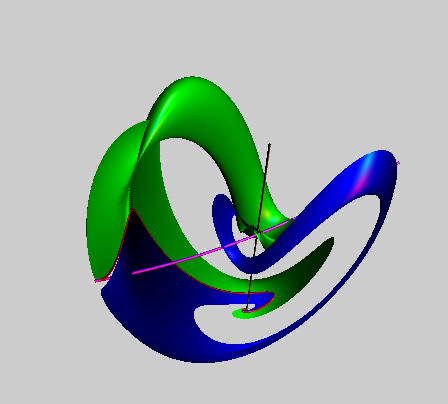
\includegraphics[height=2in]{figs/ks22manifold.ps}
\vspace*{-5pt}\caption{
{\small
	Unstable manifold of \nameit{2}~\eqv\ of KS
equation for $\tilde{L}=3.5014$, N=64 mode truncation.
	The black line represents the family of \nameit{2}~\eqva\ 
obtained by application of the translation operator, 
while the purple line represents the family of \nameit{3}~\eqva.
The red trajectory represents the heteroclinic connection from a \nameit{2}~\eqv\ to  
a \nameit{3}~\eqv.
The connection splits the manifold into two parts, 
colored blue and green here.
        } %end \small
        }
\label{f:KS22Manifold}\vspace*{-5pt}
\end{figure}
%%%%%%%%%%%%%%%%%%%%%%%%%%%%%%%%%%%%%%%%%%%%%%%%%%%%%%%%%%%%%%%%%%


Many short unstable \rpo s have been computed using Newton method.
A few of them are shown in \reffig{f:KS22rpo}.
They typically have either one unstable eigenvalue, or one complex
sigenvalue pair.
The construction 
of symbolic dynamics will allow the systematic and exhaustive determination 
of all \rpo s in the spirit of 
the earlier work presented in \refsect{s:KS} and will be a testbed 
for the trace formula with continous symmetries of \refsect{s:relativePOT}.

%%%%%%%%%%%%%%%%%%%%%%%%%%%%%%%%%%%%%%%%%%%%%%%%%%%%%%%%%%%%%%%%
\begin{figure}[h]\vspace*{-5pt}
\centering
(a)\includegraphics[width=0.2\textwidth]{figs/rpoKS21.eps}
(b)\includegraphics[width=0.2\textwidth]%,origin=c]
                {figs/rpoKS33.eps}
(c)\includegraphics[width=0.2\textwidth]%,origin=c]%
        {figs/rpoKS46.eps}
(d)\includegraphics[width=0.2\textwidth]%,origin=c]%
        {figs/rpoKS56.eps}
\vspace*{-5pt}\caption{
{\small
\Rpo s of KS
equation for $\tilde{L}=3.5014$, N=64 mode truncation.
(a) T=20.51, d=0.0 (\po),
(b) T=32.80, d=10.96,
(c) T=46.51, d=7.76,
(d) T=55.60, d=-5.25.
        } %end \small
        }
\label{f:KS22rpo}\vspace*{-5pt}
\end{figure}
%%%%%%%%%%%%%%%%%%%%%%%%%%%%%%%%%%%%%%%%%%%%%%%%%%%%%%%%%%%%%%%%%%




\section{\Rpo s}
\label{sec:rpos}
% L22rpo.tex
%
% Predrag created file              nov  2 2006
% $Author$ $Date$

\section{\Rpo s}

The \rpo s satisfy the condition $u(x+\shift,\period{}) = u(x,0)$, where $\period{}$
is the period and $\shift$ the phase shift of \rpo .  We have
limited our search to orbits with $\period{} < 200$ and found over 250 prime
orbits with $\shift \ge 0$.  Each orbit with phase shift $\shift$
has a reflection symmetric partner with phase shift $-\shift$
related by the transformation $u(x) \to -u(-x)$.

The search has not been exhaustive, and there are likely to be more
orbits with $\period{} < 200$, especially with longer periods.  However, the
orbits we've found provide a representative sample of typical \rpo s
and approximate well the chaotic attractor (since they were located
using seeds obtained from close returns within the chaotic
dynamics).

\reffig{f:ks22rposT} shows the \rpo s in the plane $(\period{},\shift)$.
\begin{figure}[t]
\begin{center}
\includegraphics[width=0.7\textwidth]{figs/ks22_rpos_Tdelta.eps}
\end{center}
\caption{\Rpo s of \KSe\ with period $\period{}$ and phase shift $\shift$.
        } \label{f:ks22rposT}
\end{figure}

The largest Lyapunov exponent of \rpo s is shown in
\reffig{f:ks22rposL}.

\begin{figure}[t]
\begin{center}
\includegraphics[width=0.7\textwidth]{figs/ks22_rpos_lyap.eps}
\end{center}
\caption{The largest Lyapunov exponent of \rpo s.
        } \label{f:ks22rposL}
\end{figure}

Next we describe several types of \rpo s.

\subsection{Short \rpo s}  The small period \rpo s outline the
coarse structure of the chaotic attractor, while the longer period
\rpo s typically just resolve the finer details of the dynamics
without significant modification of this structure.

The first five orbits with the shortest period we have found are
shown in \reffig{f:ks22rposShort}.  The shortest orbit with $\period{} =
16.4$ is also the most unstable, with one positive Lyapunov exponent
equal 0.328.  The other short orbits are less unstable, with the
largest Lyapunov exponents in the range 0.018 -- 0.073.  The
Lyapunov exponents of a \rpo are given by the formula
\[h_j = \log |\lambda_j|/\period{}\,,\]
where $\lambda_j$ are the eigenvalues of $g(\shift)J^T(a)$.  The
orbit with $\period{} = 20.5$ is exactly periodic due to a special symmetry
it possesses (see Section~\ref{ssec:po}).

\begin{figure}[t]
\begin{center}
\includegraphics[width=0.9\textwidth]{figs/ks22rposShort.eps}
%(a)\includegraphics[width=0.18\textwidth]{figs/ks22rpo016.3-02.86.eps}
%(b)\includegraphics[width=0.18\textwidth]{figs/ks22rpo020.5-00.00.eps}
%(c)\includegraphics[width=0.18\textwidth]{figs/ks22rpo032.8-10.96.eps}
%(d)\includegraphics[width=0.18\textwidth]{figs/ks22rpo033.5-04.04.eps}
%(e)\includegraphics[width=0.18\textwidth]{figs/ks22rpo034.6-09.60.eps}
\end{center}
\caption{Short period \rpo s of \KS equation with $L = 22$: (a) $\period{} =
16.3$, $\shift = 2.86$; (b) $\period{} = 20.5$, $\shift = 0.00$ (periodic
orbit); (c) $\period{} = 32.8$, $\shift = 10.96$; (d) $\period{} = 33.5$, $\shift =
4.04$; (e) $\period{} = 34.6$, $\shift = 9.60$.  Horizontal and vertical
white lines indicate periodicity and phase shift of the orbits,
respectively. }\label{f:ks22rposShort}
\end{figure}


\subsection{\Rpo s close to the unstable manifold of \EQV{2} }
We have found a number of \rpo s which stay very close to the
unstable manifold of \EQV{2}.  This confirms that the "cage" of
unstable manifolds of equilibria plays an important role in
organizing the chaotic dynamics of \KS\ equation.

\begin{figure}[t]
\begin{center}
\includegraphics[width=0.9\textwidth]{figs/ks22rposCage.eps}
\end{center}
\caption{\Rpo s close to the unstable manifold of \EQV{2}
equilibrium. (a) $\period{} = 47.6$, $\shift = 5.68$; (b) $\period{} = 55.6$,
$\shift = 5.25$; (c) $\period{} = 59.9$, $\shift = 5.44$; (d) $\period{} = 71.7$,
$\shift = 5.503$; (e) $\period{} = 85.8$, $\shift = 5.503$. Horizontal and
vertical white lines indicate periodicity and phase shift of the
orbits, respectively. }\label{f:ks22rposCage}
\end{figure}

\subsection{Periodic Orbits} \label{ssec:po}
A \rpo\ will be eventualt periodic, i.e. $\shift = 0$, if it has one of
two symmetries: 1) $-u(-x,0) = u(x,0)$ or 2) $-u(-x,\period{}/2) =
u(x,0)$.\RLD{I have the feeling that it can be proven that there are
no other types of symmetries that lead to exactly periodic
solutions, but I don't know how to construct such a proof} In the
first case the whole orbit lives within the antisymmetric subspace.
The dynamics of \KS\ equation in the antisymmetric subspace has been
investigated in [include references]. The \KS\ equation with $L =
22$ appears not to have any periodic orbits of this type.
\RLD{Is it really
so?}

The second symmetry implies that the \rpo\ is reflection-\-sym\-metric
to itself after the time translation by half the period.

We have found 22 periodic orbits 
%(POs) 
with $\period{} < 200$.  The
shortest such orbit is shown in \reffig{f:ks22rposShort}(b).  Some
of the other periodic orbits are shown in \reffig{f:ks22rposPO}. Six
of the 22 \po s were found by the same method as used for locating
\rpo s, while the other orbits were found by directly employing the
symmetry of the \po:
\[ -u(-x+d,\period{}/2) = u(x,0)\,, \quad -L/2 < d \leq L/2\,.\]
In the Fourier space representation, this symmetry is expressed as
follows
\[
 -{\bf g}(d)a^\ast(\period{}/2) = a(0)\,.
\]
This condition is used to find a \po\ with period $\period{}$ (compare it to
the condition (\ref{eq:RPOcond}) for \rpo s). 
\RLD{
It looks like there
might be many more \po s than I initially expected to find. In fact, I
can even venture a guess that there are approximately as many \po s
with symmetry (2) within $\period{} < 200$ as there are \rpo s within $\period{} <
100$. The reasoning is that it shouldn't be any harder to match
$-u(-x+d,\period{}/2)$ and $u(x,0)$, than it is to match $u(x+d,\period{})$ and
$u(x,0)$, provided the dynamics is equally mixing for all types of
orbits.  If this is true, then the number of \po s with period smaller
than $\period{}/2$ should be approximately equal to the number of \rpo s with
period smaller than $\period{}$; the equality improving with increasing
$\period{}$.
    }


\begin{figure}[t] \label{f:ks22rposPO}
\begin{center}
\includegraphics[width=0.9\textwidth]{figs/ks22rposPO.eps}
\end{center}
\caption{
\Po s of \KS\ equation with $L = 22$: (a) $\period{} =
66.8$; (b) $\period{} = 87.2$; (c) $\period{} = 95.3$; (d) $\period{} = 96.4$; (e) $\period{} =
132.6$.
        }
\end{figure}



\subsection{Energy transfer rates} % of the \KSe}
\label{sec:energyL22}
% energyL22.tex
% $Author$ $Date$

% \subsection{Symmetry invariant moments for $L=22$} % of the \KSe}
% \label{sec:energyL22}
% Predrag                   May 1 2007

%%%%%%%%%%%%%%%%%%%%%%%%%%%%%%%%%%%%%%%%%%%%%%%%%%%%%%%%%%%%%%%%
\begin{figure}[t]
\begin{center}
(a)\!\!\!\!\includegraphics[width=0.48\textwidth]{figs/energyBalancePlot.eps}%
~(b)\!\!\!\!\includegraphics[width=0.48\textwidth]{figs/energyBalancePlot.eps}
\end{center}
\caption{
(a) Power input $P$ {\em vs.}
dissipation rate $D$ 
(b) energy $E$  {\em vs.}
dissipation rate $D$,   for several  \eqva\ and \reqva,
\po s and \rpo s, and a typical ``turbulent" long-time trajectory.
System size $L=22$.
        }
\label{f:drivedrag}
\end{figure}
%%%%%%%%%%%%%%%%%%%%%%%%%%%%%%%%%%%%%%%%%%%%%%%%%%%%%%%%%%%%%%%%%%

%%%%%%%%%%%%%%%%%%%%%%%%%%%%%%%%%%%%%%%%%%%%%%%%%%%%%%%%%%%%%%%%
\begin{figure}[t]
\begin{center}
(a)\!\!\!\!\includegraphics[width=0.48\textwidth]{figs/ks22TurbConn_xfig.eps}%
~~(b)\!\!\!\!\includegraphics[width=0.48\textwidth]{figs/ks22TurbConn_xfig.eps}
\end{center}
\caption{
Two projections of the $(E,P,\dot{E})$ representation of the flow.
\EQV{1} (red), \EQV{2} (green), \EQV{3} (blue),
connections from \EQV{1} to $A(L/4)\EQV{1}$ (green),
from $A(L/4)\EQV{1}$ to \EQV{1} (yellow-green)
and from \EQV{3} to $A(L/4)\EQV{1}$ (blue), superimposed over
a generic long-time ``turbulent" trajectory (grey).
System size $L=22$.
        }
\label{f:drivedragConn}
\end{figure}
%%%%%%%%%%%%%%%%%%%%%%%%%%%%%%%%%%%%%%%%%%%%%%%%%%%%%%%%%%%%%%%%%%

\PC{
 Implementing Ruslan: all axes in \reffig{f:drivedragConn} changed by a factor
of 2?
        \\
Implementing Predrag:
label axes in \reffig{f:drivedrag}, \reffig{f:drivedragConn}
by $(E,P,D,\dot{E})$
    }
\PC{ks22TurbConn2\_xfig.eps for \reffig{f:drivedragConn}
    not checked in?
   }
\PC{\refFig{f:drivedragConn}: split into three figures, \\
    (a) label axes $(E,P)$, move to \reffig{f:drivedrag}~(b)\\
    (b) flip $y$ axis as $\dot{E}=P-D$; label axes $(P,\dot{E})$ \\
    (c) flip $y$ axis; label axes $(E,\dot{E})$ \\
   }
In \reffig{f:drivedrag}
we plot \refeq{EnRate}, the time-dependent $\dot{\expctE}$
in the
power input $P$ {\em vs.} %$\expct{u_{x}{}^2}$ vs.
dissipation rate $D$ %$\expct{u_{xx}{}^2}$
plane, for all $L=22$ \eqva\ and
\reqva\ \PCedit{determined so far},
several \po s and \rpo s, and for a typical ``turbulent"
long-time trajectory.
\PC{\reffig{f:drivedrag}:
%    (0) replace $y$-axis by
%    $\expct{(u_{xx})^2}-\expct{(u_{x})^2}$, so all \po s lie
%    on the $x$-axis and on can see more clearly the turbulent and
%    periodic trajectory, instead having them scrunched into the
%    diagonal. (a) Replace by side views of
%    3-$d$ $(\expct{u^2},\expct{(u_{x})^2},\expct{(u_{xx})^2}
%       -\expct{(u_{x})^2})$,
%    two figures;
    (b) current type figure, with chaotic trajectory,
    all \eqva, $(32.\cdots,11)$ as example of well embedded, and
    a typical \po\ {\em not} embedded into the ``turbulent" attractor.
    (c) a separate figure with more \po s, no ``turbulent" attractor.
%    (d) prepare a mathematica macro that automatically uses
%    fonts at least twice the size you use currently.
    (e) replace
    gray window with a white background, black font. (f) in the
    publication version replace colored dots with symbols of varying
    shapes, fine black border, can be filled in with colors.
    }
%\PC{In \reffig{f:drivedrag}:
%    do also try plotting the heteroclinic connections - they are
%    presumably off the diagonal
%   }
\PC{believe it or not, we are now set to compute
    $\timeAver{E}$ and $\timeAver{P}$
    using cycle expansions
    }

Projections
from the $\infty$-dimensional \statesp\ onto
the 3-dimensional
$(E,P,D)$ representation of the flow, such as
\reffigs{f:drivedrag}{f:drivedragConn},
can be misleading.
For example, the energy of \reqva\ \REQV{\pm}{2} which
seems close to the
mean turbulent energy in \reffig{f:drivedrag} is separated
from it when plotted along the
$\expct{u \, u_{x}{}^2}$ moment, where according to
\refeq{Bridges1} it takes nonzero value $c P$.
Another example is the \rpo\ $(\period{p},\shift_p) =(32.8,10.96)$
which appears well embedded within the turbulent flow.
The mean value of $\timeAver{P_p}$
evaluated on it,
\reffig{f:ks22rposShort}\,(\textit{c}),
is quite close to the long-time turbulent
time average $\timeAver{P}$.
Similarly close prediction of mean dissipation rate in the
\pCf\ from a single-period \po\ computed by
Kawahara and Kida\rf{KawKida01} has lead to
optimistic hopes that ``turbulence" is different from
low-dimensional chaos, insofar that the determination of one
magic \po\ could yield all long-time predicitions.
Regrettably, not true - as always, here too one needs a hierarchy
of \po s of increasing length to obtain accurate
predictions\rf{DasBuch}.
% \PC{\PCedit{ the Japanese heresy disposed off}}

The most one can say is that if points are clearly separated in an
$(E,P,D)$ plot (for example, in \reffig{f:ks22rposShort}
$\EQV{1}$ \eqv\ is not part of the recurrent set), they are also separated
in the full \statesp. Converse is not true - states of
very different topology can have similar energies.


    \PublicPrivate{%
        }{% switch to Private:
% leastUPO.tex
%
% Predrag created file              Apr 12 2007
% $Author$ $Date$


\subsection*{Least unstable \rpo s ???}

\ES{
The names of the \rpo\ figure files follow the convention
 {\tt rpoL-T-d.eps}s, with suffixes {\tt cm}
and {\tt u} indicating
 mean velocity frame  and $u$ representation respectively.
   }
%
Out of 30 \rpo s we
find,  only three are periodic.  The orbit
with $\period{p} = 95.25$ has a very small
$d = -6.5\,\times 10^{-7}$, but it is not periodic
(we
checked this by decreasing the integration step size and increasing the
number of modes).


%%%%%%%%%%%%%%%%%%%%%%%%%%%%%%%%%%%%%%%%%%%%%%%%%%%%%%%%%%%%%%%%
\begin{figure}[t] \label{f:rpo55}
\begin{center}
(a) \includegraphics[width=0.35\textwidth]{figs/rpo22-55-4-clean.eps}
% ./removecache.sh rpo22-55-4.eps
% abandoned rpoEq22-55-4.eps with mean velocity equilibrium embeded.
(b) \includegraphics[width=0.25\textwidth]{figs/rpoEq22-55-4-cm.eps}
\\
(c) [create rpoEq22-55-4-cm-?.eps]
\end{center}
\caption{
 The \rpo\ \REQV{+}{55} in:
 (a) \Statesp, traced for four periods $\period{p}$.
% Green curve belongs to \reffig{f:rpo55}(b) % rpo22-55-4-cm.eps
% rather than to  \reffig{f:rpo55}(a), % rpoEq22-55-4.eps?
 (b) mean velocity frame.
        The continuos family of
    {\eqva} A obtained by the action of $g$ is shown in green,
    the SA family shown in red. The \rpo\ \REQV{+}{55} stays close
    to either A or SA for close to 1/2 of {\eqv} rotation
    period, then quickly jumps to the other {\eqv} point.
 (c) mean velocity frame A, SA and \REQV{+}{55} projected on the
    $[a_?,a_?]$ plane,
    with the $\sigma x = -x$ symmetry of \KSe\ explicit.
        }
\end{figure}
%%%%%%%%%%%%%%%%%%%%%%%%%%%%%%%%%%%%%%%%%%%%%%%%%%%%%%%%%%%%%%%%%%



Sets of \rpo s are difficult to visualize simultaneously.

options:

Somewhat better visualization is in the
{\em mean velocity frame}, {\ie},
a reference frame that rotates with with velocity
$v_p=\shift_p/\period{p}$.
In the mean velocity frame a \rpo\ becomes
a \po, see  for example \refeq{f:rpo55}.
\PC{
   Update \reffig{f:rpo55}, this time project in some
   sensible states of $u$ orthogonalized frame (like
   \REQV{+}{55} eigenvectors, not Fourier components.
   }
Mean velocity frame visualization helps quite a bit.
Put a black (green, respectively) dot
twice thickness of the line every time unit; it will enable you to see
where the motion is slow and where it is fast.
% (a trick we used to understand plane Couette trajectories).
Mark the initial point on both
mean velocity \rpo\ and on \eqv\  in mean velocity
 frame with a fat triangle
indicating the direction, so we can see how they both move. Probably at the
opposite ends of the two curves - mean velocity frame is the mean motion.

%   rpo/figs/detail1rpo22-55-4.eps
%   rpo/figs/detail2rpo22-55-4.eps
%   rpo/figs/detail3rpo22-55-4.eps
%   break rpo22-55-4 into 3 parts.
%   The script for the fonts somehow crops these images

Each {\rpo} has its own mean velocity frame - and within it, {\eqv}
move on circles (or worse - because in higher Fourier modes they do more
complicated things), and it is important to know where the {\eqv} is at
a given instant.

As the shift $d$ is defined mod~$L$, better to
state for each {\rpo} its mean velocity $c_p = \shift_p/\period{p}$,
where $\shift_p$ is measured on the line (not on the circle). $c_p$ is
preferable to angle $2\pi \shift_p/L$ as it does not vary in $L \to$~large
limit (just like $\sqrt{2}$ wavelength estimate is independent of
system size).

Another convenient way to plot \eqva\ and \reqva\ on a periodic
domain $L$ is to plot
$u_x$ {\em vs.} $u$ as a curve parametrized by
$x\in [0,L]$,
as in \reffig{f:eqvSpatial}.
In this representation both \eqva\ and \reqva\ curves are
stationary, but the \reqva\ points move as functions of time.

\Po s and \rpo s can be plotted this way, as well
$u_x(x,t)$ vs. $u(x,t)$. \Po s and \rpo s  in this representation
are time-dependent `tubes,' and distances between their instantaneous
profiles possible could serve to define `nearby' orbits for
flows with continuous symmetries.

    } %end \PublicPrivate{%

% Siminos thesis summary
% $Author$ $Date$

When statistical assumptions do not hold and coherent
structures are present in extended systems
such as fluid flows, flame fronts and field theories
a dynamical description of turbulent phenomena becomes
necessary.
% Recent experimental and theoretical advances\rf{science04}
% support a dynamical vision of turbulence:
% For any finite  spatial resolution, a turbulent flow follows approximately for a finite time
% a pattern belonging to a { finite alphabet} of admissible patterns.
% The long term dynamics is a {walk through the space of these unstable patterns}.
% When statistical assumptions\rf{frisch} break down and large
% scale coherent structures are present, a dynamical description
% as a walk through a space of unstable patterns becomes natural.
% The question is how to characterize and classify such patterns?
Here we follow the seminal Hopf paper\rf{hopf48}, and  visualize
turbulence not as  a sequence of spatial snapshots in turbulent evolution,
but as a trajectory in an  $\infty$-$d$ \statesp\ in which an
instant in turbulent evolution is a {unique} point. In the dynamical systems approach,
theory of turbulence for a given system, with given boundary conditions,
is given by (a) the geometry of the \statesp\ and (b) the associated measure,
\ie, the likelihood that asymptotic dynamics visits a given \statesp\ region.

In this thesis this vision is pursued in the context of \KS\
system, one of the simplest physically interesting spatially
extended nonlinear systems. Relaxing the restriction of
previous studies\rf{LanThesis,Christiansen97} to discrete
symmetry invariant subspace a new challenge confronts our
attempt to elucidate the \statesp\ geometry. Continuous
symmetry, in the form of a subgroup of \On{n} acting on
\statesp, endows \statesp\ with additional structure.
Symmetry dictates the bifurcation structure and the type of
observed solutions. At the same time the notion recurrence becomes
relative: Not only do we have to identify points along the
orbit of the nonlinear group of time evolution but also points
along the orbit of the linear symmetry group. The latter
identification, termed symmetry reduction, although
conceptually simple as the group action is linear, is hard to
implement in practice. The high dimensionality of \statesp\
that results from truncation of a PDE is one of the reasons.
The second reason is that, for most interesting group actions,
the process introduces singularities in the structure of the
reduced \statesp.

Here we propose a procedure to efficiently project dynamics of
solutions computed in the original space to a reduced \statesp.
This is done in conjunction with eliminating time-translational
invariance with suitably chosen Poincar\'e sections to avoid
singularities while setting the stage to compute return maps
that describe how unstable manifolds of solutions organize the
flow. Simplifying the visualization of high-dimensional flows,
this procedure yields new insight into which solutions of \KSe\
are key to describing the geometry of \statesp. In context of
low-dimensional, strongly-contracting flows the procedure leads
to one-dimensional return maps that encapsulate all the
information about the dynamics.


    \PublicPrivate{%
        }{% switch to Private:
\appendix

\section{Finding \rpo s}
    % using multiple shooting and Levenberg--Marquardt algorithm}
\label{sec:lmderRLD}
\input lmderRLD

\subsection{Newton method  for \rpo\ searches}
\label{sec:NewtRPOs}
% newton.tex
%
% Predrag			jun 20 2006
% Vaggelis			may 20 2006
% $Author$ $Date$


% \section{Newton's method for determining \reqva}
% 
%  Our task is to find \reqva\ solutions of \refeq{eq:KS}.
% Although one can easilly see that this problem can be reduced to that of
%  finding periodic orbits of a 4-dimensional ODE, here we prefer to consider our system in phase space and search for solutions of
%  \beq
% 	\dot{b}_k=\dot{c}_k=0\,,
%  \eeq
%  for every $k$. The reason to do this is just getting experience before pursuing the more difficult task of locating POs and RPOs. 
%  Expanding $\dot{b}_k(a)$ and $\dot{c}_k(a)$ around our initial guess $a_o$ and demanding that they satisfy the equilibrium 
%  condition, we get
%  \bea
% 	\dot{b}_k(a) & = & \dot{b}_k(a_o)+\left.\frac{\partial \dot{b}_k}{\partial b_j}\right|_{a_o}\delta b_j + \left.\frac{\partial \dot{b}_k}{\partial c_j}\right|_{a_o}\delta c_j = 0 \continue
% 	\dot{c}_k(a) & = & \dot{c}_k(a_o)+\left.\frac{\partial \dot{c}_k}{\partial b_j}\right|_{a_o}\delta b_j + \left.\frac{\partial \dot{c}_k}{\partial c_j}\right|_{a_o}\delta c_j = 0
%  \eea
%  or in matrix form
%  \beq
%     \left( \begin{array}{cc}
%         \frac{\partial \dot{b}}{\partial b} & \frac{\partial \dot{b}}{\partial c} \\
%         \frac{\partial \dot{c}}{\partial b}	& \frac{\partial \dot{c}}{\partial c}
%      \end{array}
%      \right)_{a_o}
%      \left(\begin{array}{c}
%        \delta b  \\
%        \delta c
%      \end{array}\right)
%      =
%      \left(\begin{array}{c}
%        -\dot{b}(a_o) \\
%        -\dot{c}(a_o)
%      \end{array}\right)\,,
%      \label{eq:NewtonEquil}
% \eeq
% where $\partial{\dot{b}} / \partial{b}$ \etc are $d \times d$ submatrices. Solving this
% system of equations for the corrections $\delta b$ and  $\delta c$ and using the refined solution
% as an initial guess yields  an approximation to the solution of the system.
%  


\subsection{Implementing Newton's method  for RPOs}
\label{sec:NewtRPOs}

The relative periodic condition
\beq
	u(x+d,t+T)=u(x,t) \,
\eeq
translates in Fourier space into
\beq	
	\sum_{k=-\infty}^{+\infty} a_k (t+T) e^{ i k (x+d) / \tildeL} 
		= \sum_{k=-\infty}^{+\infty} a_k (t) e^{ i k x / \tildeL} \,
\eeq
or
\beq
	e^{ik\, d /\tildeL}a_k(t+T)=a_k(t) \,,\ \forall k \in \mathds{Z}\ \ \ \mathrm{(no\ summation)}.
	\label{eq:RPOcondition}
\eeq
We see that a relative periodic orbit returns after time $T$ to a point in 
phase space with components $a_k(t+T)$ rotated in the complex plane by an 
angle $-k\, d /\tildeL$ with respect to $a_k(t)$. In matrix notation, we write \refeq{eq:RPOcondition} as
\beq
	\mathbf{g}(d)  a(t+T)=a(t)\,,
	\label{eq:RPO}
\eeq
where we have defined
\beq
	\mathbf{g}(d) \equiv Diag[e^{ik\, d/\tildeL}]\,.
\eeq
%We notice that $R(\kappa)$ is not a rotation operator..

% Consider an initial guess $a'$ for a point on a relative periodic orbit and assume that it lies on
% a \Poincare section $\mathcal{P}$ at $t=0$. Suppose that $\mathcal{P}$ is a hyperplane in
% $\mathds{R}^{2d}$. The flow $f^t$ defined by \refeq{eq:Fcoef} transports 
% this point after time $T'$ into $a'(T')=f^{T'}(a')$. Suppose that this point is such that $R(\kappa')f^{T'}(a')$
% is a point on $\mathcal{P}$. Consider next a point $a$ lying on $\mathcal{P}$ and in the neighborhood of $a'$,
% thus satisfying
% \beq
% 	q \cdot (a'-a) = 0\,,
% 	\label{eq:cond a}
% \eeq
% with $q$ a vector normal to $\mathcal{P}$. Point $a$ will be finally identified with the improved 
% approximation of a point on the periodic orbit.
% The flow transports $a$ to $f^{T'}(a)$, but now $R(\kappa')f^{T'}(a)$ is not in general on $\mathcal{P}$.
% Moreover we would like to have the freedom to adjust the guesses for $T'$ and $\kappa'$ into new values
% $T=T'+\Delta T$ and $\kappa=\kappa'+\Delta \kappa$ to improve their accuracy. 
% Let as consider such slightly different values $T$ and $\kappa$ such that $R(\kappa)f^{T}(a)$ lies on 
% $\mathcal{P}$. Then we have the condition
% \beq
% 	q \cdot(R(\kappa')f^{T'}(a')-R(\kappa)f^{T}(a)) = 0\,.
% 	\label{eq:cond Rf(a)}
% \eeq 

Starting with an initial guess $a$ for a point on a \rpo\ we use Newton's method to find an improved approximation to the true solution $a^*$ of condition  \refeq{eq:RPO}:
\beq
	a^*=\mathbf{g}(d^*)  f^{T^*}(a^*)\,,
	\label{eq:RPOcond}
\eeq
with period $T^*$ and shift $d^*$. Let $T$ and $d$ be our guess period and shift, respectively. 
Taylor expanding $\mathbf{g}(d^*)  f^{T^*}(a^*)$ around $a$ to linear order in the small quantities 
$\delta a=a^*-a$, $\delta T=T^*-T$ and $\delta d=d^*-d$, we get
% \bea
% 	f^{T}(a)& \simeq & f^{T}(a')+\J^T(a') \Delta a \label{eq:fTaylorl1} \\ 
% 		& \simeq & f^{T'}(a') + v \Delta T + \J^{T'}(a') \Delta a \label{eq:fTaylorl2} \,, 
% \eea
% where $v$ is evaluated at $f^{T'}(a')$. Here $\J^t(x)$ is the Jacobian matrix, defined for a general flow through
% \beq
%    	J^t_{ij}(x_o)=\left.\frac{\partial x_i(t)}{\partial x_j}\right|_{x=x_0}\,.
% \eeq
% The Jacobian matrix is obtained by integrating the equation:
% \beq
%    	\dot{\mathbf{J}}^t=\mathbf{A J}^t \, ,
% 	\label{eq:Adef}
% \eeq
% subject to the initial condition:
% \beq
%    	\mathbf{J}^0=\mathbf{1} \, ,
% \eeq
% Here $\mathbf{A}$ is the matrix of variations defined as:
% \beq
% 	A_{kj}=\frac{\partial \dot{x}_k}{\partial x_j}\,.
% \eeq
% 
% In passing from \refeq{eq:fTaylorl1} to \refeq{eq:fTaylorl2} we have used the multiplicative 
% structure of the Jacobian, $\mathbf{J}^{T'+\delta T}(a')=\mathbf{J}^{\delta T}(f^{T'}(a'))\mathbf{J}^{T'}(a')$, 
% noticed that $\mathbf{J}^{\delta T}(f^{T'}(a'))=e^{\mathbf{A}\delta T}=\mathbf{1}+\mathbf{A}\delta T+\ldots$ 
% and dropped second order terms in the small quantities.
% 
% On the other hand, we have
% \bea
% 	R(\kappa'+\Delta\kappa) & = & R(\kappa')R(\Delta\kappa) \continue
% 				& \simeq & R(\kappa')(\mathbf{1}+iDiag[k]\Delta\kappa/\tildeL)\,.
% 	\label{eq:TaylorR}	
% \eea
% 
% Substituting \refeq{eq:fTaylorl2},\refeq{eq:TaylorR} into \refeq{eq:RPOcond} and keeping only first
% order terms in the small quantities, we get
% \beq
% 	a+\delta a \simeq \mathbf{g}(d)  f^{T}(a) + \mathbf{D[g]}(\mathbf{g}(d) f^{T}(a))\delta d
% 				+ \mathbf{g} (d)v(f^{T}(a)) \delta T + \mathbf{g}(d) \J^{T}(a) \delta a\,,
% \eeq
% or
\beq
	\left(\mathbf{1}-\mathbf{g}(d)\J^{T}(a)\right) \delta a - \mathbf{g}(d)v(f^{T}(a)) \delta T 
							- \mathbf{D[g]}(\mathbf{g}(d)f^{T}(a))\delta d  
					\,\simeq\, \mathbf{g}(d)f^{T}(a)-a\,,
	\label{eq:NewtonBasicCond}			
\eeq
where $D[g]_{kj}=\frac{ik}{\tildeL}\delta_{kj}$. The matrix $\mathbf{g}(d)\J^{T}(a)$ has two unit eigenvalues in 
the limit $a\rightarrow a^*$, one associated with the invariance along the direction of the flow and the other with the
translational invariance of the system. Thus \refeq{eq:NewtonBasicCond} needs to be augmented by two conditions to
eliminate the indeterminacy introduced by the (close to) zero eigenvalues of $\mathbf{1}-\mathbf{g}(d)\J^{T}(a)$. Following 
\refref{ViswanathPC06} we choose the conditions 
\bea
	v(a)\cdot\delta a & = & 0 \label{eq:NewtonAux1} \,\\
	(\mathbf{D[g]}a)\cdot \delta a & = & 0 \label{eq:NewtonAux2}\,.
\eea
The requirement imposed by \refeqs{eq:NewtonAux1}{eq:NewtonAux2}\ on the solution vector $\delta a$ of \refeq{eq:NewtonBasicCond} 
is that it vanishes along the directions of the flow and of infinitesimal translation of the initial condition.

Equations \refeq{eq:NewtonBasicCond} and \refeqs{eq:NewtonAux1}{eq:NewtonAux2}
can be compactly represented in a single matrix equation:
\beq
    \left( \begin{array}{ccc}
       \mathbf{1}-\mathbf{g}(d)\mathbf{J}^{T}(a) 	& -\mathbf{g}(d)v(f^{T}(a))	  & -\mathbf{D[g]}(\mathbf{g}(d)f^{T}(a))  \\
        v(a)^{\dagger}			& 0  	& 0 	\\
        (\mathbf{D[g]}a)^\dagger	& 0 	& 0 
     \end{array}
     \right)
     \left(\begin{array}{c}
       \delta a \\
       \delta T \\
       \delta d
     \end{array}\right)
     =
     \left(\begin{array}{c}
       \mathbf{g}(d)f^{T}(a)-a \\
       0     \\
       0
     \end{array}\right)\,.
     \label{eq:NewtonScheme}
\eeq
where $v^\dagger$ denotes the adjoint of $v$. 

\JFG{Back around \ref{expan} in fourier.tex you mentioned you set the 
coefficients to purely imaginary values $i a_k$ and fixed $a_{-k}= -
a_k$ to assure real-valuedness and to isolate antisymmetric solutions. 
This eliminates continuous translation symmetries. Presumably in this
section, since you're looking for RPOs, this is relaxed. Do you then
enforce real-valuedness in your Newton-descent via the constraint
$a_{-k} = a^*{k}$ (the conjugates that then appear in the equations
are nondifferentiable which is a big pain) or do you let the solutions
go complex and then choose the real part at the end? The cost of that
is that the dimension of your search space is twice as big as it needs 
to be. That's an unacceptable cost in fluids; perhaps in KS it's not. 
In any case, I think you should (1) either clarify that you're no 
longer working in the antisymmetric subspace or eliminate its mention 
earlier, and (2) explain how you ultimately arrive at real-valued 
solutions.}


\input fourierRLD
\newpage
    } %end \PublicPrivate{%
\PC{
    If there is only {\em one} appendix, however,  % \verb|\Appendix|
    (with a capital letter) should be used: produces only
    the word {\bf Appendix} in the section title.
   }

%\PCedit{acknowledgement directly before references}
\section*{Acknowledgments}
% ackn.tex
% $Author$ $Date$

We thank Y.~Lan for determining
the $L=22$ \EQV{1}~\eqv.

% \PC{PC.bib wasd temporary, now incorporated into ../bibtex/siminos.bib}

\bibliography{../bibtex/siminos}

    \PublicPrivate{%
        }{% switch to Private:
\newpage
% siminos/atlas/flotsam.tex    master file: main.tex
% $Author$ $Date$

\section{Flotsam}
\label{s:flotsam}

\subsection{Pipe flows}
\label{s:review}
% former siminos/atlas/review.tex    master file: main.tex

As long as one is focusing on a single solution of \NSe, there are many
excellent, physically insightful $3D$ visualizations of the flow:
velocity fields on flow sections, isovorticity surfaces, videos of the
flow, and so on. But today we own dozens of exact \eqv\ and \reqv\
solutions for a given turbulent flow, and we are commencing an exploration of
states of turbulent fluids in terms of the unstable \po\ solutions whose
number, as a function of the increasing period, is growing exponentially.
How are we to visualize \emph{the totality} of these solutions in one go?

The answer was given by \cite{hopf48}, who envisioned the function space
of {\NS} velocity fields as an infinite-dimensional \statesp\ $\pS$ in
which each instantaneous state of $3D$ fluid velocity field $\vec{u}(\bx)$ is
represented as a unique point $\ssp$. In our particular application we
can represent $\ssp = (\vec{u}_{nkm})$ as a vector whose elements are the
primitive discretization variables \refeq{pipeDiscr}. The $3D$ velocity
field given by $\vec{u}_{knm}(\zeit)$, obtained from integration of the
\NSe\ in time, can hence be seen as trajectory $\ssp(\zeit)$ in
$\approx 100,000$ dimensional space spanned by the free variables of our
numerical discretization, with the \NS\ equations \refeq{NavStokesDev}
rewritten as
\beq
   \dot{\ssp} = \vel(\ssp) ,
   \qquad
   \ssp(\zeit) = \ssp(0)
            + \int_0^\zeit \! \mathrm{d}\zeit' \, \vel(\ssp(\zeit'))
\,,
\ee{symbolicNS}
where the current state of the fluid $ \ssp(\zeit)$ is the time-$\zeit$
forward map of the initial fluid state  $\ssp(0)$.

In order to quantify whether two fluid states are close to or far from
each other, one needs a notion of distance between two points in
\statesp, measured here as
\beq
  \Norm{\ssp-\ssp'}^2  = \braket{\ssp-\ssp'}{\ssp-\ssp'} =
\frac{1}{V}
\int_\bCell \! d \bx \;
(\vec{u}-\vec{u}') \cdot (\vec{u}-\vec{u}')
\,.
\ee{innerproduct}
There is no compelling reason to use this {`energy norm'}, other than
that velocity fields is what is given in a numerical computation. What
norm one actually uses depends very much on the application.
Visualizations of trajectory \refeq{symbolicNS} are of necessity
projections onto two or three dimensions.

Recently, \cite{GHCW07} have shown that the dynamics of different regions
of {\statesp}, considered as a high-dimensional vector space,
can be elucidated more profitably by a computationally
straight\-forward sets of \emph{physical} coordinates. One identifies
several prominent states of the flow $\vec{u}_A$, $\vec{u}_B$, $\dots$, such as
{\eqv} states and their linearized stability eigenvectors, states in whose neighborhoods the
turbulent flow spends most of the time, and from them constructs, by
Gram-Schmidt or (anti)-symmetrizations, an orthonormal basis set
$\{\be_1, \be_2, \cdots, \be_n\}$. The evolving fluid state $\bu(\zeit)$
is then projected onto this basis using the inner product
\refeq{innerproduct},
\beq
\ssp(\zeit) =(\ssp_1, \ssp_2, \cdots, \ssp_n, \cdots)(\zeit)
    \,,\qquad
\ssp_n(\zeit) = \braket{\vec{u}(\zeit)}{\be_n}
\,.
\ee{intrSspTraj}
Low-dimensional projections of the flow can be viewed in any of the $2D$ planes
$(\ssp_m, \ssp_n)$ or in $3D$ perspective views $(\ssp_{\ell},\ssp_m,
\ssp_n)$. An example is the \reffig{f:MeanVelocityFrame} projection on
the $3$\dmn\ frame $\{{\be}_1,{\be}_2,{\be}_3\}$ defined in \refeq{FrenetFrame1}.
It is worth emphasizing that the method affords low-dimensional {\em
visualization} without any low-dimensional {\em modeling} or dimension
reduction; the dynamics are computed with fully-resolved direct numerical
simulations.

Such visualizations are a prerequisite to uncovering the
interrelations between (the infinite number of) invariant solutions, and
constructing symbolic dynamics partitions of \statesp\ needed for a
systematic exploration of turbulent dynamics, the key challenge that we
address here for the case of turbulent pipe flows.


\subsection{Symmetries of pipe flow}
\label{s:SymmPipe}
% former siminos/atlas/symm.tex



Let $\LieEl(\phi,\shift)$ be the shift operator such that $\LieEl(\phi,0)$
denotes an azimuthal rotation by $\phi$ about the pipe axis,
and $\LieEl(0,\shift)$ denotes the stream-wise translation by
$\shift$; let $\sigma$ denote reflection about the $\theta=0$ azimuthal
angle:
\bea
\LieEl(\phi,\shift) \, [u,v,w,p](r,\theta,z)
        & = & [u,v,w,p](r,\theta-\phi,z-\shift)
			  \continue
\sigma \, [u,v,w,p](r,\theta,z) \;\; & = & [u,-v,w,p](r,-\theta,z)
\label{pipeSymms}
\eea
%
The \NSe\ for pipe flow are equivariant under these transformations. The
symmetry group of stream-wise periodic pipe flow is thus $\Group =
\On{2}_\theta \times \SOn{2}_z = \Dn{1} \ltimes \SOn{2}_{\theta} \times
\SOn{2}_z$, where $\Dn{1} = \{ e,\, \sigma \}$ denotes azimuthal
reflection, $\ltimes$ stands for a semi-direct product (in general,
reflections and rotations do not commute), and the subscripts $z,\theta$
indicate stream-wise translation and azimuthal rotation respectively.

In the literature
(see, \eg\ \cite{Recke2010}) such \SOn{2} is often referred to as the
circle group $S^1$, also denoted `one-torus' $T^1$.

\section{How to slice}
\label{s:algorithm}

\refFig{fig:sliceimage}, new proposal: take points on the good,
    blue \po, run each along the group orbit until $\sspRSing \in S$
    where it intersects the \sliceBord, see \refeq{sspRSing}, and thus plot
    the border of where the local slice ends, once on the left, and once
    on the right of the {\template}. Catch - I have not thought this
    through, not sure that the condition \refeq{sspRSing} can be
    satisfied on every group orbit...

\subsection{Rotation into the \slice}

As long as the norm is discretization independent, the \slice\ condition
\refeq{PCsectQ0} is independent of the numerical representation $\ssp$ of
the flow $\vec{u}$, be it finite difference, spectral, and so on. The
slice condition is solved for $\shift$ every few time steps using
Newton's method, where a good initial guess for $\shift(\zeit)$ is
obtained from the previous value and $\dot{\shift}(\zeit)$.

To avoid this, a global
atlas has to be pieced together from local \slice\ charts, fixed by
a well-chosen set of
\template s $\slicep{}^{(j)}$.
Shifts $\shift_j(\zeit)$ are tracked for each local \slice\ chart $\pS{}^{(j)}$,
such that the next $\shift_{j+1}(\zeit)$ is selected at intersection with
$\pS{}^{(j+1)}$
to minimise $\Norm{{\ssp}-{\ssp_i}}$.

%\APW{111104 The first sentence requires simplifying!}
As group orbits % of compact Lie groups
are smooth manifolds, have natural linear
representations (under linear action of a symmetry group, \statesp\
decomposes into a sum over irreducible subspaces), and have natural local
coordinate frames (the group tangent, curvature Frenet-Serret frames
\refeq{FrenetFrame}), good \slice s should be easier to construct than
the elusive ``good'' Poincar\'e sections of the time-evolution flows.
Indeed, as a generic \slice\ \refeq{PCsectQ0} is the set of all
group-orbit points closest to a given {\template}, it slices the group
orbits of \emph{all} full \statesp\ points\rf{FrCv11}. However, for a
nonlinear flow, there is no single \slice\ that really does the job: our
\slice\ is locally a hyperplane, expected to be a good description of
solutions similar to a given {\template} in some open neighborhood. The
variational distance condition \refeq{PCsectQ0} is only an extremum
condition, and as the group orbits of highly nonlinear states are highly
contorted (see \reffig{fig:2830GO6}\,(b)), they can have many
extrema, and multiple sections by a \slice\ hyperplane. For example, an
\rpo\  torus is always intersected by a \slice\ hyperplane in two or more
sections, see \reffig{fig:sliceimage}.
    \PC{\refFig{fig:sliceimage}, new proposal: take points on the good,
    blue \po, run each along the group orbit until $\sspRSing \in S$
    where it intersects the \sset, see \refeq{sspRSing}, and thus plot
    the border of where the local slice ends, once on the left, and once
    on the right of the {\template}. Catch - I have not thought this
    through, not sure that the condition \refeq{sspRSing} can be
    satisfied on every group orbit...
    }


\subsection{Dynamically important solutions and Newton's method}
\label{s:reqva}

The way in which the \mslices\ enables to find initial
guesses for $(\vec{u}(0),\period{},\shift)$, is the main differences
between this study and the previous ones.

Here we take as initial guesses samples of nearly recurrent velocity
fields generated by long-time simulations of turbulent dynamics
\rf{pchaot,CviGib10}. The intent is to find the {\em dynamically most
important} solutions, by sampling the turbulent flow's natural measure.
In practice, sufficiently good full \statesp\ initial guesses for
$(\vec{u}(0),\period{},\shift)$ would be almost impossible to find.
Checking correlations between $\vec{u}(\zeit)$ and
$\LieEl(0,\shift)\,\vec{u}(\zeit-\period{})$ for each $\period{}$, and
more problematically, for all possible shifts $(\phi,\shift)$, is an
unrealistic task. The \mslices, however, enables us determine close
recurrences  from the symmetry-reduced time series, and locates the
dynamically most important solutions, \ie, those trajectories that are
most likely to be observed in a long-time turbulent simulation. The \rpo
s are reduced to \po s, whose unstable manifolds are much easier to track
in the \reducedsp. The \rpo\ shift $\shift$ is given by the
reconstruction equation, \refeq{reconstrEq}, or, in practice, by phase
shift $\shift(\period{})-\shift(0)$ accumulated by the intermediate
Newton steps that keep the orbit within the slice.

Without symmetry reduction, the detection of the nearest recurrence of a
state near a previous state, earlier on the the same trajectory, would
require the calculating the minimum over all possible shifts. Within the
symmetry-\reducedsp\ the determination of recurrences is simple, as the
slices are constructed by requiring that the slice points are the minimum
distance points between the group orbits of the two states.

\section*{Uncertainty estimates and $L_2$ bounds for the Kuramoto-Sivashinsky equation}

Jared C. Bronski
%\footnote{Department of Mathematics,
% University of Illinois Urbana-Champaign, 1409 W. Green St, Urbana IL 61801}\\
and
Tom Gambill

importance as a model for flame fronts\cite{siv} and
phase turbulence\cite{KS}
and plasmas\cite{LMRT} the
KS equation has become
one of the canonical models for
spatio-temporal chaos in $1\!+\!1$ dimensions
\cite{JOHNSON,KEVREKIDIS,Man}.

Nicolaenko, Scheurer and Temam\cite{NICO} gave the first long-time
boundedness result for the Kuramoto-Sivashinsky equation, showing
 that $\limsup_{t \rightarrow \infty} |\!|u|\!|_2
\le C L^{\frac{5}{2}}$
for odd initial data, as well as showing
that bounds on the $L_2$ norm imply bounds on the dimension of the attractor.

The $L_2$ estimate was improved by
Collet, Eckmann, Epstein and
Stubbe\cite{CEES} who  extended it to any mean-zero initial data and improved the exponent from
$\frac{5}{2}$ to $\frac{8}{5}$,
and by Goodman\cite{Good}, who extended it to
any mean-zero initial data with the same exponent.

these papers that the function $|\!|u-\phi|\!|_2^2$ is a Lyapunov function for
an appropriately chosen $\phi$ and $|\!|u|\!|_2$ sufficiently large.

bounds which do not fit into Lyapunov function framework:
Ilyashenko\cite{Ilyashenko},
Otto  and Giacomelli\cite{GO}.
The latter, which treats the KS equation as a
perturbation of the Burger's equation, is currently the best estimate, establishing that
\[
\limsup_{t \rightarrow \infty} |\!|u|\!|_2 = o(L^{\frac{3}{2}}).
\]

In this paper we give an elementary argument of the Lyapunov function
type which establishes the slightly weaker result
\[
\limsup_{t \rightarrow \infty} |\!|u|\!|_2 = O(L^{\frac{3}{2}}).
\]
Our proof applies equally to the destabilized Kuramoto-Sivashinsky (dKS)
equation:
\[
u_t = -u_{xxxx} - u_{xx} + \gamma  u + u u_x ~~~~~~\gamma > 0 ~~~~~ \int u(x,0)dx = 0.
\]

It was shown by Wittenberg\cite{WITTENBERG} that this equation
has stationary solutions which satisfy $|\!|u|\!| \propto L^{\frac{3}{2}}.$
Since a Lyapunov function argument for the KS equation also applies
to the dKS equation (for sufficiently small $\gamma$) Wittenberg
argued that $\frac{3}{2}$ is the best exponent that one can expect
from the Lyapunov function approach.

Similar ideas of
considerably greater generality have been used by Constantin and Doering
to establish bounds on energy dissipation in fluids, and generally
go by the name `background flow method.'\cite{CD1,CD2}

The basic strategy is to choose a
periodic function $\phi_x$ of zero mean such that the following
quadratic form is coercive,
\[
<\!\!u, K u\!\!>= \int u_{xx}^2 - u_x^2 + \phi_x u^2 \ge \delta |\!|u|\!|^2,
\]
for $u$ satisfying Dirichlet boundary conditions and some positive
$\delta$ independent of $L$.

This calculation is, in a sense, complementary to Lieb-Thirring type
inequalities.
In Lieb-Thirring inequalities one attempts to maximize some measure of the
negative part of the spectrum of an operator over all potentials with
a fixed norm.



P. Constantin, C. Foias, B. Nicolaenko and R. Temam,
    Integral Manifolds and Inertial Manifolds for
    Dissipative Partial differential Equations,
    Applied Mathematics Sciences 70 (1989), Springer-Verlag.

C. Foias and I. Kukavica, Determing nodes for the Kuramoto-Sivashinsky equation, J. Dynam. Di. Eq. 7 (1995), 365-373.

J. Goodman, Stability of the Kuramoto-Sivashinsky equation and related systems, Comm. Pure Appl. Math 47 (1994), 293-306.

M.S. Jolly, I.G. Kevrekidis and E.S. Titi, Approximate inertial manifolds for the Kuramoto-Sivashinsky equation:analysis and computations, Physica D 44 (1990), 38-60.

D. Michelson, Elementary particles as solutions of the Sivashinksky equations, Physica D 44 (1990), 502-556.

E. Mitidieri and S.I. Pohozaev, Apriori Estimates and Blow-up of Solutions to Nonlinear Partial Differential Equations and Inequalities, Procedings of the Steklov Institute of Mathematics Issue 3 vol 234 (2001).

Y.CAO AND E.S. TITI

Y. Pomeau and P. Manneville, Stability and fluctuations of spatially periodic flow, J. Physique Lett. 40 (1979), 609-612.

G. Sell and M. Taboada Local dissipativity and attractors for the Kuramoto-Sivashinsky equation in thin 2D domains, Nonlinear Anal. 18 (1992), 671-687.

P. Souplet, Gradient blow-up for multidimensional nonlinear parabolic equations with general boundary conditions, Di. Inegral Eqns 15 (2002), 237-56.

E. Tadmor, The well-posedness of the Kuramoto-Sivashinsky equation, SIAM Journal on Mathematical analysis 17 (1986), 884-893.


article{CEES}
Collet, P., Eckmann, J.-P., Epstein, H. and Stubbe, J. (1993).
A Global Attracting Set for the Kuramoto-Sivashinsky Equation.
{\it Comm. Math. Phys.}
{\bf 152}, ~203-214.

article{CD1} Constantin, P. and Doering, C. (1992).
Energy dissipation in shear driven turbulence.
{\it Phys. Rev. Lett.} {\bf 69} (11), 1648-1651.

article{CD2} Constantin, P. and Doering, C. (1995).
Variational Bounds for Dissipative Systems.
{\it Phys. D}, {\bf 82} (3), 221-228.

article{Foias}
Foias, C.,Manley, O. and Temam, R. (1987).
Attractors for the B\'{e}nard problem:
Existence and physical bounds on their fractal dimensions.
{\it Nonlinear Anal.}
{\bf 11}, ~939-967.

article{Foias2}
Foias, C., Sell, G. R., and  Temam, R. (1988).
Inertial manifolds for nonlinear evolutionary equations.
{\it J. Diff. Eq.}
{\bf 73} (2), ~309-353.

article{Good}
Goodman, J. (1994).
Stability of the Kuramoto-Sivashinsky and Related Systems.
{\it Comm. Pure Appl. Math.}
{\bf 47} (3), ~293-306.

article{Ilyashenko}
Il\'{}yashenko, Yu. S. (1992).
Global analysis of the phase portrait for the Kuramoto-Sivashinsky equation.
{\it J. Dynam. Diff. Eq.}
{\bf 4}  (4), ~585-615.

article{JOHNSON}
 Johnson, M. E., Jolly, M. S., and  Kevrekidis, I. G. (2001).
The Oseberg transition: visualization of global bifurcations for the
Kuramoto-Sivashinsky equation.
{\it Internat. J. Bifur. Chaos Appl. Sci. Engrg.}
{\bf 11} (1), ~1-18.

article{LMRT} LaQuey, R., Mahajan, S., Rutherford, P. and Tang, W. (1975).
{\it Phys. Rev. Lett} {\bf 34} (7) 391-394.


article{Man} Manneville, P. (1989).
{\it Dissipative Structures and Weak Turbulence} Academic Press, San Francisco/London.

article{NICO}
Nicolaenko B.,Scheurer, B., and Temam, R. (1985).
Some Global Dynamical Properties of the Kuramoto-Sivashinsky Equations: Nonlinear Stability and Attractors.
{\it Phys. D}
{\bf 16} (2), 155-183.

article{ST} Sell, G. and Taboada, M. (1992).
 Local dissipativity and attractors for the Kuramoto-Sivashinsky
equation in thin $2{\rm D}$ domains.
{\it Nonlinear Analysis} {\bf 18} (7), 671-687.

article{Temam}
Temam, Roger (1988)
{\itshape Infinite Dimensional Dynamical Systems in Mechanics and Physics},
Springer, Berlin/Heidelberg/New York.

article{WITTENBERG}
Wittenberg, R. W.(2002).
Dissipativity, analyticity and viscous shocks in the (de)stabilized
Kuramoto-Sivashinsky equation.
{\it Phys. Lett. A}
{\bf 300} (4-5), 407-416.
  % on bounds
    } %end \PublicPrivate{%

\end{document}
